\documentclass[12pt, a4paper]{report}

% ── packages ──────────────────────────────────────────────────────────────────
\usepackage[T1]{fontenc}
\usepackage[utf8]{inputenc}
\usepackage[a4paper, margin=2.5cm]{geometry}
\usepackage{graphicx}
\usepackage{booktabs}
\usepackage{multirow}
\usepackage{amsmath}
\usepackage{amssymb}
\usepackage{xcolor}
\usepackage[hidelinks]{hyperref}
\usepackage{microtype}
\usepackage{siunitx}
\usepackage{subcaption}
\usepackage{setspace}
\usepackage{fancyhdr}
\usepackage{tikz}
\usepackage[section]{placeins}
\sisetup{reset-text-series=false, text-series-to-math=true}
\onehalfspacing

% ── figure paths ──────────────────────────────────────────────────────────────
\graphicspath{{../../results/}{figures/}}

% ── convenience ───────────────────────────────────────────────────────────────
\newcommand{\tbd}{\textcolor{gray}{--}}
\newcommand{\na}{\textcolor{gray}{n/a}}

% ── graceful fallbacks for auto-generated metrics ─────────────────────────────
\providecommand{\whuGAITCnnTestAcc}{\tbd}
\providecommand{\whuGAITAuthTestAUC}{\tbd}
\providecommand{\whuGAITSimplDAUC}{\tbd}
\providecommand{\whuGAITSimplDTPRone}{\tbd}
\providecommand{\whuGAITSimplDTPRten}{\tbd}
\providecommand{\whuGAITComboASR}{\tbd}
\providecommand{\whuGAITBudgetRatio}{\tbd}
\providecommand{\uciharCnnTestAcc}{\tbd}
\providecommand{\uciharAuthTestAUC}{\tbd}
\providecommand{\uciharSimplDAUC}{\tbd}
\providecommand{\uciharSimplDTPRone}{\tbd}
\providecommand{\uciharSimplDTPRten}{\tbd}
\providecommand{\uciharComboASR}{\tbd}
\providecommand{\wisdmCnnTestAcc}{\tbd}
\providecommand{\wisdmAuthTestAUC}{\tbd}
\providecommand{\wisdmSimplDAUC}{\tbd}
\providecommand{\wisdmSimplDTPRone}{\tbd}
\providecommand{\wisdmSimplDTPRten}{\tbd}
\providecommand{\wisdmComboASR}{\tbd}
\providecommand{\combinedAuthTestAUC}{\tbd}
\providecommand{\combinedSimplDAUC}{\tbd}
\providecommand{\combinedSimplDTPRone}{\tbd}
\providecommand{\combinedSimplDTPRten}{\tbd}
\providecommand{\signalAuthModelAUCB}{\tbd}
\providecommand{\signalAuthModelAUCA}{\tbd}
\providecommand{\signalAuthModelAUCC}{\tbd}
\providecommand{\signalMiaAUCBvsC}{\tbd}
\providecommand{\signalMiaAUCAvsC}{\tbd}
\providecommand{\signalConfusionThresholdFPRten}{\tbd}

% ── auto-generated metric fallbacks ─────────────────────────────────────────
\providecommand{\baselineAlreadyAccepted}{\tbd}
\providecommand{\baselinePdiff}{\tbd}
\providecommand{\combinedAuthDiffMean}{\tbd}
\providecommand{\combinedAuthOverfitAcc}{\tbd}
\providecommand{\combinedAuthSameMean}{\tbd}
\providecommand{\combinedAuthSep}{\tbd}
\providecommand{\combinedAuthTestAcc}{\tbd}
\providecommand{\combinedAuthTrainAcc}{\tbd}
\providecommand{\combinedBudgetRatio}{\tbd}
\providecommand{\combinedCnnTestAcc}{\tbd}
\providecommand{\combinedComboASR}{\tbd}
\providecommand{\combinedEpsTarget}{\tbd}
\providecommand{\combinedMemberUci}{\tbd}
\providecommand{\combinedMemberWhu}{\tbd}
\providecommand{\combinedMemberWis}{\tbd}
\providecommand{\combinedMiaAUC}{\tbd}
\providecommand{\combinedMiaDfiveDiffPairCorr}{\tbd}
\providecommand{\combinedMiaDfiveSamePairCorr}{\tbd}
\providecommand{\combinedMiaDeltaGap}{\tbd}
\providecommand{\combinedMiaLFauc}{\tbd}
\providecommand{\combinedMiaMFauc}{\tbd}
\providecommand{\combinedMiaMemberAggregateDelta}{\tbd}
\providecommand{\combinedMiaMemberAttributed}{\tbd}
\providecommand{\combinedMiaMemberDeltaMean}{\tbd}
\providecommand{\combinedMiaMemberDeltaStd}{\tbd}
\providecommand{\combinedMiaMemberDiffMean}{\tbd}
\providecommand{\combinedMiaMemberN}{\tbd}
\providecommand{\combinedMiaMemberSameMean}{\tbd}
\providecommand{\combinedMiaMemberTotal}{\tbd}
\providecommand{\combinedMiaNonMemberAggregateDelta}{\tbd}
\providecommand{\combinedMiaNonMemberAttributed}{\tbd}
\providecommand{\combinedMiaNonMemberDeltaMean}{\tbd}
\providecommand{\combinedMiaNonMemberDeltaStd}{\tbd}
\providecommand{\combinedMiaNonMemberDiffMean}{\tbd}
\providecommand{\combinedMiaNonMemberN}{\tbd}
\providecommand{\combinedMiaNonMemberSameMean}{\tbd}
\providecommand{\combinedMiaOptFPR}{\tbd}
\providecommand{\combinedMiaOptTPR}{\tbd}
\providecommand{\combinedMiaOptThr}{\tbd}
\providecommand{\combinedMiaOptimalFPR}{\tbd}
\providecommand{\combinedMiaOptimalTPR}{\tbd}
\providecommand{\combinedMiaOptimalThreshold}{\tbd}
\providecommand{\combinedMiaTPRaten}{\tbd}
\providecommand{\combinedMiaTPRattwenty}{\tbd}
\providecommand{\combinedMiaTPRatFPRten}{\tbd}
\providecommand{\combinedMiaTPRatFPRtwenty}{\tbd}
\providecommand{\combinedNCombos}{\tbd}
\providecommand{\combinedNFullCombos}{\tbd}
\providecommand{\combinedNPairs}{\tbd}
\providecommand{\combinedNResistant}{\tbd}
\providecommand{\combinedNonmemberUci}{\tbd}
\providecommand{\combinedNonmemberWis}{\tbd}
\providecommand{\combinedSimplDDeltaGap}{\tbd}
\providecommand{\combinedTestPairs}{\tbd}
\providecommand{\combinedTotalMembers}{\tbd}
\providecommand{\combinedTotalNonmembers}{\tbd}
\providecommand{\combinedTrainBudgetRatio}{\tbd}
\providecommand{\combinedTrainComboASR}{\tbd}
\providecommand{\combinedTrainPairs}{\tbd}
\providecommand{\comboDiffLtwoMax}{\tbd}
\providecommand{\comboDiffLtwoMedian}{\tbd}
\providecommand{\comboDiffLtwoMin}{\tbd}
\providecommand{\comboDiffLtwoQone}{\tbd}
\providecommand{\comboDiffLtwoQthree}{\tbd}
\providecommand{\datasetName}{\tbd}
\providecommand{\detectionDistinguish}{\tbd}
\providecommand{\detectionPValue}{\tbd}
\providecommand{\epsFloor}{\tbd}
\providecommand{\epsGridN}{\tbd}
\providecommand{\epsTarget}{\tbd}
\providecommand{\epsTargetMethod}{\tbd}
\providecommand{\featureCloserFrac}{\tbd}
\providecommand{\featureMeanRatio}{\tbd}
\providecommand{\floorFracPct}{\tbd}
\providecommand{\gridStepRatio}{\tbd}
\providecommand{\hfrAdvMean}{\tbd}
\providecommand{\hfrCleanMean}{\tbd}
\providecommand{\kBestEps}{\tbd}
\providecommand{\kBestMeanEpsMin}{\tbd}
\providecommand{\kConvergenceRatio}{\tbd}
\providecommand{\kOriginal}{\tbd}
\providecommand{\kValues}{\tbd}
\providecommand{\ltwoSameMean}{\tbd}
\providecommand{\ltwoSamePten}{\tbd}
\providecommand{\ltwoSamePninety}{\tbd}
\providecommand{\nBisect}{\tbd}
\providecommand{\nImpostorCombos}{\tbd}
\providecommand{\nImpostorPairsTest}{\tbd}
\providecommand{\nSampleAblation}{\tbd}
\providecommand{\nSampleSpectral}{\tbd}
\providecommand{\signalMiaAUCAvsCCold}{\tbd}
\providecommand{\signalMiaAUCAvsCLira}{\tbd}
\providecommand{\signalMiaAUCBvsCCold}{\tbd}
\providecommand{\signalMiaAUCBvsCLira}{\tbd}
\providecommand{\signalAuthModelAUCD}{\tbd}
\providecommand{\signalMiaAUCDvsC}{\tbd}
\providecommand{\signalMiaAUCDvsCLira}{\tbd}
\providecommand{\signalMiaAUCDvsCCold}{\tbd}
\providecommand{\signalMiaInteractionDiff}{\tbd}
\providecommand{\signalMiaInteractionSuperAdditive}{\tbd}
\providecommand{\signalConfusionTPRC}{\tbd}
\providecommand{\signalConfusionTPRA}{\tbd}
\providecommand{\signalConfusionTPRB}{\tbd}
\providecommand{\signalConfusionTPRD}{\tbd}
\providecommand{\signalConfusionThresholdFPRten}{\tbd}
% four-case authenticator metrics
\providecommand{\whugaitFourCaseMMAcc}{\tbd}
\providecommand{\whugaitFourCaseMMAuc}{\tbd}
\providecommand{\whugaitFourCaseNNAcc}{\tbd}
\providecommand{\whugaitFourCaseNNAuc}{\tbd}
\providecommand{\whugaitFourCaseMNAcc}{\tbd}
\providecommand{\whugaitFourCaseNMAcc}{\tbd}
\providecommand{\whugaitFourCaseAucGap}{\tbd}
\providecommand{\whugaitFourCaseAccGap}{\tbd}
\providecommand{\uciharFourCaseMMAcc}{\tbd}
\providecommand{\uciharFourCaseMMAuc}{\tbd}
\providecommand{\uciharFourCaseNNAcc}{\tbd}
\providecommand{\uciharFourCaseNNAuc}{\tbd}
\providecommand{\uciharFourCaseMNAcc}{\tbd}
\providecommand{\uciharFourCaseNMAcc}{\tbd}
\providecommand{\uciharFourCaseAucGap}{\tbd}
\providecommand{\uciharFourCaseAccGap}{\tbd}
\providecommand{\wisdmFourCaseMMAcc}{\tbd}
\providecommand{\wisdmFourCaseMMAuc}{\tbd}
\providecommand{\wisdmFourCaseNNAcc}{\tbd}
\providecommand{\wisdmFourCaseNNAuc}{\tbd}
\providecommand{\wisdmFourCaseMNAcc}{\tbd}
\providecommand{\wisdmFourCaseNMAcc}{\tbd}
\providecommand{\wisdmFourCaseAucGap}{\tbd}
\providecommand{\wisdmFourCaseAccGap}{\tbd}
% simple-delta threshold metrics
\providecommand{\miaAUC}{\tbd}
\providecommand{\miaMeanThr}{\tbd}
\providecommand{\miaMeanTPR}{\tbd}
\providecommand{\miaMeanFPR}{\tbd}
\providecommand{\miaOptThr}{\tbd}
\providecommand{\miaOptTPR}{\tbd}
\providecommand{\miaOptFPR}{\tbd}
\providecommand{\uciharMiaAUC}{\tbd}
\providecommand{\uciharMiaMeanTPR}{\tbd}
\providecommand{\uciharMiaMeanFPR}{\tbd}
\providecommand{\uciharMiaOptTPR}{\tbd}
\providecommand{\uciharMiaOptFPR}{\tbd}
\providecommand{\uciharMiaMeanThr}{\tbd}
\providecommand{\uciharMiaOptThr}{\tbd}
\providecommand{\wisdmMiaAUC}{\tbd}
\providecommand{\wisdmMiaMeanTPR}{\tbd}
\providecommand{\wisdmMiaMeanFPR}{\tbd}
\providecommand{\wisdmMiaOptTPR}{\tbd}
\providecommand{\wisdmMiaOptFPR}{\tbd}
\providecommand{\wisdmMiaMeanThr}{\tbd}
\providecommand{\wisdmMiaOptThr}{\tbd}
% hidden-layer centroid delta threshold metrics
\providecommand{\hiddenDeltaAUC}{\tbd}
\providecommand{\hiddenMeanTPR}{\tbd}
\providecommand{\hiddenMeanFPR}{\tbd}
\providecommand{\hiddenOptTPR}{\tbd}
\providecommand{\hiddenOptFPR}{\tbd}
\providecommand{\hiddenMeanThr}{\tbd}
\providecommand{\hiddenOptThr}{\tbd}
\providecommand{\uciharHiddenMeanTPR}{\tbd}
\providecommand{\uciharHiddenMeanFPR}{\tbd}
\providecommand{\uciharHiddenOptTPR}{\tbd}
\providecommand{\uciharHiddenOptFPR}{\tbd}
\providecommand{\uciharHiddenMeanThr}{\tbd}
\providecommand{\uciharHiddenOptThr}{\tbd}
\providecommand{\wisdmHiddenDeltaAUC}{\tbd}
\providecommand{\wisdmHiddenMeanTPR}{\tbd}
\providecommand{\wisdmHiddenMeanFPR}{\tbd}
\providecommand{\wisdmHiddenOptTPR}{\tbd}
\providecommand{\wisdmHiddenOptFPR}{\tbd}
\providecommand{\wisdmHiddenMeanThr}{\tbd}
\providecommand{\wisdmHiddenOptThr}{\tbd}
\providecommand{\whuGAITGreyLiraRawAUC}{\tbd}
\providecommand{\whuGAITGreyLiraRawTPRten}{\tbd}
\providecommand{\whuGAITColdLiraRawAUC}{\tbd}
\providecommand{\whuGAITColdLiraRawTPRten}{\tbd}
\providecommand{\whuGAITColdLiraLfAUC}{\tbd}
\providecommand{\whuGAITColdLiraLfTPRten}{\tbd}
\providecommand{\whuGAITColdLiraMfAUC}{\tbd}
\providecommand{\whuGAITColdLiraMfTPRten}{\tbd}
\providecommand{\whuGAITWarmLiraRawAUC}{\tbd}
\providecommand{\whuGAITWarmLiraRawTPRten}{\tbd}
\providecommand{\uciharGreyLiraRawAUC}{\tbd}
\providecommand{\uciharGreyLiraRawTPRten}{\tbd}
\providecommand{\uciharColdLiraRawAUC}{\tbd}
\providecommand{\uciharColdLiraRawTPRten}{\tbd}
\providecommand{\uciharColdLiraLfAUC}{\tbd}
\providecommand{\uciharColdLiraLfTPRten}{\tbd}
\providecommand{\uciharColdLiraMfAUC}{\tbd}
\providecommand{\uciharColdLiraMfTPRten}{\tbd}
\providecommand{\uciharWarmLiraRawAUC}{\tbd}
\providecommand{\uciharWarmLiraRawTPRten}{\tbd}
\providecommand{\wisdmGreyLiraRawAUC}{\tbd}
\providecommand{\wisdmGreyLiraRawTPRten}{\tbd}
\providecommand{\wisdmColdLiraRawAUC}{\tbd}
\providecommand{\wisdmColdLiraRawTPRten}{\tbd}
\providecommand{\wisdmColdLiraLfAUC}{\tbd}
\providecommand{\wisdmColdLiraLfTPRten}{\tbd}
\providecommand{\wisdmColdLiraMfAUC}{\tbd}
\providecommand{\wisdmColdLiraMfTPRten}{\tbd}
\providecommand{\wisdmWarmLiraRawAUC}{\tbd}
\providecommand{\wisdmWarmLiraRawTPRten}{\tbd}
\providecommand{\combinedGreyLiraRawAUC}{\tbd}
\providecommand{\combinedGreyLiraRawTPRten}{\tbd}
\providecommand{\combinedColdLiraRawAUC}{\tbd}
\providecommand{\combinedColdLiraRawTPRten}{\tbd}
\providecommand{\combinedColdLiraLfAUC}{\tbd}
\providecommand{\combinedColdLiraLfTPRten}{\tbd}
\providecommand{\combinedColdLiraMfAUC}{\tbd}
\providecommand{\combinedColdLiraMfTPRten}{\tbd}
\providecommand{\combinedWarmLiraRawAUC}{\tbd}
\providecommand{\combinedWarmLiraRawTPRten}{\tbd}
\providecommand{\whuGAITHiddenDeltaAUC}{\tbd}
\providecommand{\uciharHiddenDeltaAUC}{\tbd}
\providecommand{\wisdmHiddenDeltaAUC}{\tbd}
\providecommand{\combinedHiddenDeltaAUC}{\tbd}
% cl_mia chapter fallbacks
\providecommand{\clMiaCLMIAStdAUC}{\tbd}
\providecommand{\clMiaCLMIACdmlAUC}{\tbd}
\providecommand{\clMiaCLMIAStdMemDelta}{\tbd}
\providecommand{\clMiaCLMIACdmlMemDelta}{\tbd}
\providecommand{\clMiaCLMIAStdNMDelta}{\tbd}
\providecommand{\clMiaCLMIACdmlNMDelta}{\tbd}
\providecommand{\clMiaCLMIAStdSep}{\tbd}
\providecommand{\clMiaCLMIACdmlSep}{\tbd}
\providecommand{\clMiaCLMIAAUCGap}{\tbd}
\providecommand{\clMiaCLStdAuthAcc}{\tbd}
\providecommand{\clMiaCLCdmlAuthAcc}{\tbd}
\providecommand{\whuGAITPgdMiaAUC}{\tbd}
\providecommand{\uciharPgdMiaAUC}{\tbd}
\providecommand{\wisdmPgdMiaAUC}{\tbd}
\providecommand{\combinedPgdMiaAUC}{\tbd}
\providecommand{\spectralFCutoff}{\tbd}
\providecommand{\spectralFracInBand}{\tbd}
\providecommand{\uciharAuthDiffMean}{\tbd}
\providecommand{\uciharAuthOverfitAcc}{\tbd}
\providecommand{\uciharAuthSameMean}{\tbd}
\providecommand{\uciharAuthSep}{\tbd}
\providecommand{\uciharAuthTestAcc}{\tbd}
\providecommand{\uciharAuthTrainAcc}{\tbd}
\providecommand{\uciharBudgetRatio}{\tbd}
\providecommand{\uciharEpsTarget}{\tbd}
\providecommand{\uciharNCombos}{\tbd}
\providecommand{\uciharNFullCombos}{\tbd}
\providecommand{\uciharNPairs}{\tbd}
\providecommand{\uciharNResistant}{\tbd}
\providecommand{\uciharSimplDDeltaGap}{\tbd}
\providecommand{\uciharTrainBudgetRatio}{\tbd}
\providecommand{\uciharTrainComboASR}{\tbd}
\providecommand{\whuGAITAuthDiffMean}{\tbd}
\providecommand{\whuGAITAuthOverfitAcc}{\tbd}
\providecommand{\whuGAITAuthSameMean}{\tbd}
\providecommand{\whuGAITAuthSep}{\tbd}
\providecommand{\whuGAITAuthTestAcc}{\tbd}
\providecommand{\whuGAITAuthTrainAcc}{\tbd}
\providecommand{\whuGAITEpsTarget}{\tbd}
\providecommand{\whuGAITNCombos}{\tbd}
\providecommand{\whuGAITNFullCombos}{\tbd}
\providecommand{\whuGAITNPairs}{\tbd}
\providecommand{\whuGAITNResistant}{\tbd}
\providecommand{\whuGAITSimplDDeltaGap}{\tbd}
\providecommand{\whuGAITTrainBudgetRatio}{\tbd}
\providecommand{\whuGAITTrainComboASR}{\tbd}
\providecommand{\wisdmAuthDiffMean}{\tbd}
\providecommand{\wisdmAuthOverfitAcc}{\tbd}
\providecommand{\wisdmAuthSameMean}{\tbd}
\providecommand{\wisdmAuthSep}{\tbd}
\providecommand{\wisdmAuthTestAcc}{\tbd}
\providecommand{\wisdmAuthTrainAcc}{\tbd}
\providecommand{\wisdmBudgetRatio}{\tbd}
\providecommand{\wisdmEpsTarget}{\tbd}
\providecommand{\wisdmNCombos}{\tbd}
\providecommand{\wisdmNFullCombos}{\tbd}
\providecommand{\wisdmNPairs}{\tbd}
\providecommand{\wisdmNResistant}{\tbd}
\providecommand{\wisdmSimplDDeltaGap}{\tbd}
\providecommand{\wisdmTrainBudgetRatio}{\tbd}
\providecommand{\wisdmTrainComboASR}{\tbd}

% ── auto-generated metrics ────────────────────────────────────────────────────
\IfFileExists{../generated/compare_models_whuGAIT_metrics.tex}
  {% Auto-generated by compare_models_whuGAIT: DO NOT EDIT MANUALLY
% Last run: 2026-09-25 13:50:03

\providecommand{\whugaitFourCaseMMAcc}{}
\renewcommand{\whugaitFourCaseMMAcc}{95.55\%}
\providecommand{\whugaitFourCaseMMAuc}{}
\renewcommand{\whugaitFourCaseMMAuc}{0.9890}
\providecommand{\whugaitFourCaseNNAcc}{}
\renewcommand{\whugaitFourCaseNNAcc}{78.26\%}
\providecommand{\whugaitFourCaseNNAuc}{}
\renewcommand{\whugaitFourCaseNNAuc}{0.8451}
\providecommand{\whugaitFourCaseMNAcc}{}
\renewcommand{\whugaitFourCaseMNAcc}{86.06\%}
\providecommand{\whugaitFourCaseNMAcc}{}
\renewcommand{\whugaitFourCaseNMAcc}{87.12\%}
\providecommand{\whugaitFourCaseAucGap}{}
\renewcommand{\whugaitFourCaseAucGap}{+0.1439}
\providecommand{\whugaitFourCaseAccGap}{}
\renewcommand{\whugaitFourCaseAccGap}{+17.29pp}
}{}
\IfFileExists{../generated/compare_models_ucihar_metrics.tex}
  {% Auto-generated by compare_models_ucihar: DO NOT EDIT MANUALLY
% Last run: 2026-09-25 13:50:03

\providecommand{\uciharFourCaseMMAcc}{}
\renewcommand{\uciharFourCaseMMAcc}{90.98\%}
\providecommand{\uciharFourCaseMMAuc}{}
\renewcommand{\uciharFourCaseMMAuc}{0.9611}
\providecommand{\uciharFourCaseNNAcc}{}
\renewcommand{\uciharFourCaseNNAcc}{69.34\%}
\providecommand{\uciharFourCaseNNAuc}{}
\renewcommand{\uciharFourCaseNNAuc}{0.7538}
\providecommand{\uciharFourCaseMNAcc}{}
\renewcommand{\uciharFourCaseMNAcc}{78.98\%}
\providecommand{\uciharFourCaseNMAcc}{}
\renewcommand{\uciharFourCaseNMAcc}{80.16\%}
\providecommand{\uciharFourCaseAucGap}{}
\renewcommand{\uciharFourCaseAucGap}{+0.2073}
\providecommand{\uciharFourCaseAccGap}{}
\renewcommand{\uciharFourCaseAccGap}{+21.64pp}
}{}
\IfFileExists{../generated/compare_models_wisdm_metrics.tex}
  {% Auto-generated by compare_models_wisdm: DO NOT EDIT MANUALLY
% Last run: 2026-09-25 13:50:03

\providecommand{\wisdmFourCaseMMAcc}{}
\renewcommand{\wisdmFourCaseMMAcc}{98.12\%}
\providecommand{\wisdmFourCaseMMAuc}{}
\renewcommand{\wisdmFourCaseMMAuc}{0.9958}
\providecommand{\wisdmFourCaseNNAcc}{}
\renewcommand{\wisdmFourCaseNNAcc}{93.49\%}
\providecommand{\wisdmFourCaseNNAuc}{}
\renewcommand{\wisdmFourCaseNNAuc}{0.9822}
\providecommand{\wisdmFourCaseMNAcc}{}
\renewcommand{\wisdmFourCaseMNAcc}{93.70\%}
\providecommand{\wisdmFourCaseNMAcc}{}
\renewcommand{\wisdmFourCaseNMAcc}{92.12\%}
\providecommand{\wisdmFourCaseAucGap}{}
\renewcommand{\wisdmFourCaseAucGap}{+0.0136}
\providecommand{\wisdmFourCaseAccGap}{}
\renewcommand{\wisdmFourCaseAccGap}{+4.63pp}
}{}
\IfFileExists{../generated/compare_models_combined_metrics.tex}
  {% Auto-generated by compare_models_combined: DO NOT EDIT MANUALLY
% Last run: 2026-09-25 13:50:03

\providecommand{\combinedFourCaseMMAcc}{}
\renewcommand{\combinedFourCaseMMAcc}{82.22\%}
\providecommand{\combinedFourCaseMMAuc}{}
\renewcommand{\combinedFourCaseMMAuc}{0.9373}
\providecommand{\combinedFourCaseNNAcc}{}
\renewcommand{\combinedFourCaseNNAcc}{73.36\%}
\providecommand{\combinedFourCaseNNAuc}{}
\renewcommand{\combinedFourCaseNNAuc}{0.8288}
\providecommand{\combinedFourCaseMNAcc}{}
\renewcommand{\combinedFourCaseMNAcc}{79.50\%}
\providecommand{\combinedFourCaseNMAcc}{}
\renewcommand{\combinedFourCaseNMAcc}{73.80\%}
\providecommand{\combinedFourCaseAucGap}{}
\renewcommand{\combinedFourCaseAucGap}{+0.1085}
\providecommand{\combinedFourCaseAccGap}{}
\renewcommand{\combinedFourCaseAccGap}{+8.86pp}
}{}
\IfFileExists{../generated/nb05a_metrics.tex}
  {% Auto-generated by nb05a: DO NOT EDIT MANUALLY
% Last run: 2026-09-24 15:13:00

\providecommand{\miaMeanTPR}{}
\renewcommand{\miaMeanTPR}{0.776}
\providecommand{\miaMeanFPR}{}
\renewcommand{\miaMeanFPR}{0.050}
\providecommand{\miaOptTPR}{}
\renewcommand{\miaOptTPR}{0.939}
\providecommand{\miaOptFPR}{}
\renewcommand{\miaOptFPR}{0.100}
}{}
\IfFileExists{../generated/nb05a_ucihar_metrics.tex}
  {% Auto-generated by nb05a_ucihar: DO NOT EDIT MANUALLY
% Last run: 2026-09-24 18:28:51

\providecommand{\uciharMiaMeanTPR}{}
\renewcommand{\uciharMiaMeanTPR}{0.810}
\providecommand{\uciharMiaMeanFPR}{}
\renewcommand{\uciharMiaMeanFPR}{0.000}
\providecommand{\uciharMiaOptTPR}{}
\renewcommand{\uciharMiaOptTPR}{0.810}
\providecommand{\uciharMiaOptFPR}{}
\renewcommand{\uciharMiaOptFPR}{0.000}
}{}
\IfFileExists{../generated/nb05a_wisdm_metrics.tex}
  {% Auto-generated by nb05a_wisdm: DO NOT EDIT MANUALLY
% Last run: 2026-09-25 02:38:46

\providecommand{\wisdmMiaMeanTPR}{}
\renewcommand{\wisdmMiaMeanTPR}{0.700}
\providecommand{\wisdmMiaMeanFPR}{}
\renewcommand{\wisdmMiaMeanFPR}{0.000}
\providecommand{\wisdmMiaOptTPR}{}
\renewcommand{\wisdmMiaOptTPR}{0.800}
\providecommand{\wisdmMiaOptFPR}{}
\renewcommand{\wisdmMiaOptFPR}{0.000}
}{}
\IfFileExists{../generated/nb05a_combined_metrics.tex}
  {% Auto-generated by nb05a_combined: DO NOT EDIT MANUALLY
% Last run: 2026-09-25 07:05:35

\providecommand{\combinedMiaMeanTPR}{}
\renewcommand{\combinedMiaMeanTPR}{0.736}
\providecommand{\combinedMiaMeanFPR}{}
\renewcommand{\combinedMiaMeanFPR}{0.400}
\providecommand{\combinedMiaOptTPR}{}
\renewcommand{\combinedMiaOptTPR}{0.615}
\providecommand{\combinedMiaOptFPR}{}
\renewcommand{\combinedMiaOptFPR}{0.067}
}{}
\IfFileExists{../generated/nb05a_hidden_metrics.tex}
  {% Auto-generated by nb05a_hidden: DO NOT EDIT MANUALLY
% Last run: 2026-09-24 15:13:36

\providecommand{\hiddenMeanTPR}{}
\renewcommand{\hiddenMeanTPR}{0.633}
\providecommand{\hiddenMeanFPR}{}
\renewcommand{\hiddenMeanFPR}{0.100}
\providecommand{\hiddenOptTPR}{}
\renewcommand{\hiddenOptTPR}{0.959}
\providecommand{\hiddenOptFPR}{}
\renewcommand{\hiddenOptFPR}{0.200}
}{}
\IfFileExists{../generated/nb05a_hidden_ucihar_metrics.tex}
  {% Auto-generated by nb05a_hidden_ucihar: DO NOT EDIT MANUALLY
% Last run: 2026-09-24 18:29:10

\providecommand{\uciharHiddenMeanTPR}{}
\renewcommand{\uciharHiddenMeanTPR}{0.619}
\providecommand{\uciharHiddenMeanFPR}{}
\renewcommand{\uciharHiddenMeanFPR}{0.000}
\providecommand{\uciharHiddenOptTPR}{}
\renewcommand{\uciharHiddenOptTPR}{1.000}
\providecommand{\uciharHiddenOptFPR}{}
\renewcommand{\uciharHiddenOptFPR}{0.333}
}{}
\IfFileExists{../generated/nb05a_hidden_wisdm_metrics.tex}
  {% Auto-generated by nb05a_hidden_wisdm: DO NOT EDIT MANUALLY
% Last run: 2026-09-25 02:39:04

\providecommand{\wisdmHiddenMeanTPR}{}
\renewcommand{\wisdmHiddenMeanTPR}{0.475}
\providecommand{\wisdmHiddenMeanFPR}{}
\renewcommand{\wisdmHiddenMeanFPR}{0.455}
\providecommand{\wisdmHiddenOptTPR}{}
\renewcommand{\wisdmHiddenOptTPR}{0.950}
\providecommand{\wisdmHiddenOptFPR}{}
\renewcommand{\wisdmHiddenOptFPR}{0.455}
}{}
\IfFileExists{../generated/nb05a_hidden_combined_metrics.tex}
  {% Auto-generated by nb05a_hidden_combined: DO NOT EDIT MANUALLY
% Last run: 2026-09-25 07:05:43

\providecommand{\combinedHiddenMeanTPR}{}
\renewcommand{\combinedHiddenMeanTPR}{0.659}
\providecommand{\combinedHiddenMeanFPR}{}
\renewcommand{\combinedHiddenMeanFPR}{0.367}
\providecommand{\combinedHiddenOptTPR}{}
\renewcommand{\combinedHiddenOptTPR}{0.604}
\providecommand{\combinedHiddenOptFPR}{}
\renewcommand{\combinedHiddenOptFPR}{0.167}
}{}
\IfFileExists{../generated/compare_mia_whuGAIT_metrics.tex}
  {% Auto-generated by compare_mia_whuGAIT: DO NOT EDIT MANUALLY
% Last run: 2026-09-25 13:50:11

\providecommand{\whuGAITSimplDAUC}{}
\renewcommand{\whuGAITSimplDAUC}{0.959}
\providecommand{\whuGAITSimplDDeltaGap}{}
\renewcommand{\whuGAITSimplDDeltaGap}{0.337}
\providecommand{\whuGAITSimplDTPRten}{}
\renewcommand{\whuGAITSimplDTPRten}{0.939}
\providecommand{\whuGAITGreyLiraRawAUC}{}
\renewcommand{\whuGAITGreyLiraRawAUC}{0.905}
\providecommand{\whuGAITGreyLiraRawACC}{}
\renewcommand{\whuGAITGreyLiraRawACC}{0.746}
\providecommand{\whuGAITGreyLiraRawTPRten}{}
\renewcommand{\whuGAITGreyLiraRawTPRten}{0.714}
\providecommand{\whuGAITGreyLiraLfAUC}{}
\renewcommand{\whuGAITGreyLiraLfAUC}{0.806}
\providecommand{\whuGAITGreyLiraLfACC}{}
\renewcommand{\whuGAITGreyLiraLfACC}{0.542}
\providecommand{\whuGAITGreyLiraLfTPRten}{}
\renewcommand{\whuGAITGreyLiraLfTPRten}{0.469}
\providecommand{\whuGAITGreyLiraMfAUC}{}
\renewcommand{\whuGAITGreyLiraMfAUC}{0.856}
\providecommand{\whuGAITGreyLiraMfACC}{}
\renewcommand{\whuGAITGreyLiraMfACC}{0.644}
\providecommand{\whuGAITGreyLiraMfTPRten}{}
\renewcommand{\whuGAITGreyLiraMfTPRten}{0.592}
\providecommand{\whuGAITWarmLiraRawAUC}{}
\renewcommand{\whuGAITWarmLiraRawAUC}{0.488}
\providecommand{\whuGAITWarmLiraRawACC}{}
\renewcommand{\whuGAITWarmLiraRawACC}{0.822}
\providecommand{\whuGAITWarmLiraRawTPRten}{}
\renewcommand{\whuGAITWarmLiraRawTPRten}{0.051}
\providecommand{\whuGAITColdLiraRawAUC}{}
\renewcommand{\whuGAITColdLiraRawAUC}{0.693}
\providecommand{\whuGAITColdLiraRawACC}{}
\renewcommand{\whuGAITColdLiraRawACC}{0.847}
\providecommand{\whuGAITColdLiraRawTPRten}{}
\renewcommand{\whuGAITColdLiraRawTPRten}{0.418}
\providecommand{\whuGAITColdLiraLfAUC}{}
\renewcommand{\whuGAITColdLiraLfAUC}{0.693}
\providecommand{\whuGAITColdLiraLfACC}{}
\renewcommand{\whuGAITColdLiraLfACC}{0.831}
\providecommand{\whuGAITColdLiraLfTPRten}{}
\renewcommand{\whuGAITColdLiraLfTPRten}{0.378}
\providecommand{\whuGAITColdLiraMfAUC}{}
\renewcommand{\whuGAITColdLiraMfAUC}{0.787}
\providecommand{\whuGAITColdLiraMfACC}{}
\renewcommand{\whuGAITColdLiraMfACC}{0.839}
\providecommand{\whuGAITColdLiraMfTPRten}{}
\renewcommand{\whuGAITColdLiraMfTPRten}{0.561}
}{}
\IfFileExists{../generated/compare_mia_ucihar_metrics.tex}
  {% Auto-generated by compare_mia_ucihar: DO NOT EDIT MANUALLY
% Last run: 2026-09-25 13:50:11

\providecommand{\uciharSimplDAUC}{}
\renewcommand{\uciharSimplDAUC}{0.937}
\providecommand{\uciharSimplDDeltaGap}{}
\renewcommand{\uciharSimplDDeltaGap}{0.391}
\providecommand{\uciharSimplDTPRten}{}
\renewcommand{\uciharSimplDTPRten}{0.810}
\providecommand{\uciharGreyLiraRawAUC}{}
\renewcommand{\uciharGreyLiraRawAUC}{0.825}
\providecommand{\uciharGreyLiraRawACC}{}
\renewcommand{\uciharGreyLiraRawACC}{0.633}
\providecommand{\uciharGreyLiraRawTPRten}{}
\renewcommand{\uciharGreyLiraRawTPRten}{0.476}
\providecommand{\uciharGreyLiraLfAUC}{}
\renewcommand{\uciharGreyLiraLfAUC}{0.884}
\providecommand{\uciharGreyLiraLfACC}{}
\renewcommand{\uciharGreyLiraLfACC}{0.700}
\providecommand{\uciharGreyLiraLfTPRten}{}
\renewcommand{\uciharGreyLiraLfTPRten}{0.571}
\providecommand{\uciharGreyLiraMfAUC}{}
\renewcommand{\uciharGreyLiraMfAUC}{0.788}
\providecommand{\uciharGreyLiraMfACC}{}
\renewcommand{\uciharGreyLiraMfACC}{0.767}
\providecommand{\uciharGreyLiraMfTPRten}{}
\renewcommand{\uciharGreyLiraMfTPRten}{0.667}
\providecommand{\uciharWarmLiraRawAUC}{}
\renewcommand{\uciharWarmLiraRawAUC}{0.841}
\providecommand{\uciharWarmLiraRawACC}{}
\renewcommand{\uciharWarmLiraRawACC}{0.733}
\providecommand{\uciharWarmLiraRawTPRten}{}
\renewcommand{\uciharWarmLiraRawTPRten}{0.476}
\providecommand{\uciharColdLiraRawAUC}{}
\renewcommand{\uciharColdLiraRawAUC}{0.952}
\providecommand{\uciharColdLiraRawACC}{}
\renewcommand{\uciharColdLiraRawACC}{0.700}
\providecommand{\uciharColdLiraRawTPRten}{}
\renewcommand{\uciharColdLiraRawTPRten}{0.857}
\providecommand{\uciharColdLiraLfAUC}{}
\renewcommand{\uciharColdLiraLfAUC}{0.952}
\providecommand{\uciharColdLiraLfACC}{}
\renewcommand{\uciharColdLiraLfACC}{0.700}
\providecommand{\uciharColdLiraLfTPRten}{}
\renewcommand{\uciharColdLiraLfTPRten}{0.810}
\providecommand{\uciharColdLiraMfAUC}{}
\renewcommand{\uciharColdLiraMfAUC}{0.942}
\providecommand{\uciharColdLiraMfACC}{}
\renewcommand{\uciharColdLiraMfACC}{0.700}
\providecommand{\uciharColdLiraMfTPRten}{}
\renewcommand{\uciharColdLiraMfTPRten}{0.762}
}{}
\IfFileExists{../generated/compare_mia_wisdm_metrics.tex}
  {% Auto-generated by compare_mia_wisdm: DO NOT EDIT MANUALLY
% Last run: 2026-09-25 13:50:11

\providecommand{\wisdmSimplDAUC}{}
\renewcommand{\wisdmSimplDAUC}{0.895}
\providecommand{\wisdmSimplDDeltaGap}{}
\renewcommand{\wisdmSimplDDeltaGap}{0.095}
\providecommand{\wisdmSimplDTPRten}{}
\renewcommand{\wisdmSimplDTPRten}{0.875}
\providecommand{\wisdmGreyLiraRawAUC}{}
\renewcommand{\wisdmGreyLiraRawAUC}{0.907}
\providecommand{\wisdmGreyLiraRawACC}{}
\renewcommand{\wisdmGreyLiraRawACC}{0.843}
\providecommand{\wisdmGreyLiraRawTPRten}{}
\renewcommand{\wisdmGreyLiraRawTPRten}{0.825}
\providecommand{\wisdmGreyLiraLfAUC}{}
\renewcommand{\wisdmGreyLiraLfAUC}{0.702}
\providecommand{\wisdmGreyLiraLfACC}{}
\renewcommand{\wisdmGreyLiraLfACC}{0.431}
\providecommand{\wisdmGreyLiraLfTPRten}{}
\renewcommand{\wisdmGreyLiraLfTPRten}{0.300}
\providecommand{\wisdmGreyLiraMfAUC}{}
\renewcommand{\wisdmGreyLiraMfAUC}{0.816}
\providecommand{\wisdmGreyLiraMfACC}{}
\renewcommand{\wisdmGreyLiraMfACC}{0.588}
\providecommand{\wisdmGreyLiraMfTPRten}{}
\renewcommand{\wisdmGreyLiraMfTPRten}{0.500}
\providecommand{\wisdmWarmLiraRawAUC}{}
\renewcommand{\wisdmWarmLiraRawAUC}{0.700}
\providecommand{\wisdmWarmLiraRawACC}{}
\renewcommand{\wisdmWarmLiraRawACC}{0.804}
\providecommand{\wisdmWarmLiraRawTPRten}{}
\renewcommand{\wisdmWarmLiraRawTPRten}{0.300}
\providecommand{\wisdmColdLiraRawAUC}{}
\renewcommand{\wisdmColdLiraRawAUC}{0.814}
\providecommand{\wisdmColdLiraRawACC}{}
\renewcommand{\wisdmColdLiraRawACC}{0.784}
\providecommand{\wisdmColdLiraRawTPRten}{}
\renewcommand{\wisdmColdLiraRawTPRten}{0.325}
\providecommand{\wisdmColdLiraLfAUC}{}
\renewcommand{\wisdmColdLiraLfAUC}{0.773}
\providecommand{\wisdmColdLiraLfACC}{}
\renewcommand{\wisdmColdLiraLfACC}{0.784}
\providecommand{\wisdmColdLiraLfTPRten}{}
\renewcommand{\wisdmColdLiraLfTPRten}{0.450}
\providecommand{\wisdmColdLiraMfAUC}{}
\renewcommand{\wisdmColdLiraMfAUC}{0.811}
\providecommand{\wisdmColdLiraMfACC}{}
\renewcommand{\wisdmColdLiraMfACC}{0.784}
\providecommand{\wisdmColdLiraMfTPRten}{}
\renewcommand{\wisdmColdLiraMfTPRten}{0.525}
}{}
\IfFileExists{../generated/compare_mia_combined_metrics.tex}
  {% Auto-generated by compare_mia_combined: DO NOT EDIT MANUALLY
% Last run: 2026-09-25 13:50:11

\providecommand{\combinedSimplDAUC}{}
\renewcommand{\combinedSimplDAUC}{0.750}
\providecommand{\combinedSimplDDeltaGap}{}
\renewcommand{\combinedSimplDDeltaGap}{0.230}
\providecommand{\combinedSimplDTPRten}{}
\renewcommand{\combinedSimplDTPRten}{0.626}
\providecommand{\combinedGreyLiraRawAUC}{}
\renewcommand{\combinedGreyLiraRawAUC}{0.726}
\providecommand{\combinedGreyLiraRawACC}{}
\renewcommand{\combinedGreyLiraRawACC}{0.438}
\providecommand{\combinedGreyLiraRawTPRten}{}
\renewcommand{\combinedGreyLiraRawTPRten}{0.286}
\providecommand{\combinedGreyLiraLfAUC}{}
\renewcommand{\combinedGreyLiraLfAUC}{0.668}
\providecommand{\combinedGreyLiraLfACC}{}
\renewcommand{\combinedGreyLiraLfACC}{0.364}
\providecommand{\combinedGreyLiraLfTPRten}{}
\renewcommand{\combinedGreyLiraLfTPRten}{0.187}
\providecommand{\combinedGreyLiraMfAUC}{}
\renewcommand{\combinedGreyLiraMfAUC}{0.734}
\providecommand{\combinedGreyLiraMfACC}{}
\renewcommand{\combinedGreyLiraMfACC}{0.455}
\providecommand{\combinedGreyLiraMfTPRten}{}
\renewcommand{\combinedGreyLiraMfTPRten}{0.308}
\providecommand{\combinedWarmLiraRawAUC}{}
\renewcommand{\combinedWarmLiraRawAUC}{0.636}
\providecommand{\combinedWarmLiraRawACC}{}
\renewcommand{\combinedWarmLiraRawACC}{0.736}
\providecommand{\combinedWarmLiraRawTPRten}{}
\renewcommand{\combinedWarmLiraRawTPRten}{0.297}
\providecommand{\combinedColdLiraRawAUC}{}
\renewcommand{\combinedColdLiraRawAUC}{0.659}
\providecommand{\combinedColdLiraRawACC}{}
\renewcommand{\combinedColdLiraRawACC}{0.752}
\providecommand{\combinedColdLiraRawTPRten}{}
\renewcommand{\combinedColdLiraRawTPRten}{0.000}
\providecommand{\combinedColdLiraLfAUC}{}
\renewcommand{\combinedColdLiraLfAUC}{0.646}
\providecommand{\combinedColdLiraLfACC}{}
\renewcommand{\combinedColdLiraLfACC}{0.752}
\providecommand{\combinedColdLiraLfTPRten}{}
\renewcommand{\combinedColdLiraLfTPRten}{0.000}
\providecommand{\combinedColdLiraMfAUC}{}
\renewcommand{\combinedColdLiraMfAUC}{0.768}
\providecommand{\combinedColdLiraMfACC}{}
\renewcommand{\combinedColdLiraMfACC}{0.752}
\providecommand{\combinedColdLiraMfTPRten}{}
\renewcommand{\combinedColdLiraMfTPRten}{0.000}
}{}
\IfFileExists{../generated/compare_evasion_whuGAIT_metrics.tex}
  {% Auto-generated by compare_evasion_whuGAIT: DO NOT EDIT MANUALLY
% Last run: 2026-09-25 13:50:18

\providecommand{\whuGAITEpsTarget}{}
\renewcommand{\whuGAITEpsTarget}{25.49}
\providecommand{\whuGAITComboASR}{}
\renewcommand{\whuGAITComboASR}{0.999}
\providecommand{\whuGAITBudgetRatio}{}
\renewcommand{\whuGAITBudgetRatio}{0.098}
\providecommand{\whuGAITNResistant}{}
\renewcommand{\whuGAITNResistant}{7}
\providecommand{\whuGAITNPairs}{}
\renewcommand{\whuGAITNPairs}{5000}
\providecommand{\whuGAITNFullCombos}{}
\renewcommand{\whuGAITNFullCombos}{373}
\providecommand{\whuGAITNCombos}{}
\renewcommand{\whuGAITNCombos}{380}
\providecommand{\whuGAITTrainComboASR}{}
\renewcommand{\whuGAITTrainComboASR}{0.999}
\providecommand{\whuGAITTrainBudgetRatio}{}
\renewcommand{\whuGAITTrainBudgetRatio}{0.146}
}{}
\IfFileExists{../generated/compare_evasion_ucihar_metrics.tex}
  {% Auto-generated by compare_evasion_ucihar: DO NOT EDIT MANUALLY
% Last run: 2026-09-25 13:50:18

\providecommand{\uciharEpsTarget}{}
\renewcommand{\uciharEpsTarget}{37.47}
\providecommand{\uciharComboASR}{}
\renewcommand{\uciharComboASR}{0.995}
\providecommand{\uciharBudgetRatio}{}
\renewcommand{\uciharBudgetRatio}{0.138}
\providecommand{\uciharNResistant}{}
\renewcommand{\uciharNResistant}{27}
\providecommand{\uciharNPairs}{}
\renewcommand{\uciharNPairs}{5000}
\providecommand{\uciharNFullCombos}{}
\renewcommand{\uciharNFullCombos}{53}
\providecommand{\uciharNCombos}{}
\renewcommand{\uciharNCombos}{72}
\providecommand{\uciharTrainComboASR}{}
\renewcommand{\uciharTrainComboASR}{0.992}
\providecommand{\uciharTrainBudgetRatio}{}
\renewcommand{\uciharTrainBudgetRatio}{0.177}
}{}
\IfFileExists{../generated/compare_evasion_wisdm_metrics.tex}
  {% Auto-generated by compare_evasion_wisdm: DO NOT EDIT MANUALLY
% Last run: 2026-09-25 13:50:18

\providecommand{\wisdmEpsTarget}{}
\renewcommand{\wisdmEpsTarget}{31.00}
\providecommand{\wisdmComboASR}{}
\renewcommand{\wisdmComboASR}{0.979}
\providecommand{\wisdmBudgetRatio}{}
\renewcommand{\wisdmBudgetRatio}{0.351}
\providecommand{\wisdmNResistant}{}
\renewcommand{\wisdmNResistant}{106}
\providecommand{\wisdmNPairs}{}
\renewcommand{\wisdmNPairs}{5000}
\providecommand{\wisdmNFullCombos}{}
\renewcommand{\wisdmNFullCombos}{85}
\providecommand{\wisdmNCombos}{}
\renewcommand{\wisdmNCombos}{110}
\providecommand{\wisdmTrainComboASR}{}
\renewcommand{\wisdmTrainComboASR}{0.963}
\providecommand{\wisdmTrainBudgetRatio}{}
\renewcommand{\wisdmTrainBudgetRatio}{0.366}
}{}
\IfFileExists{../generated/compare_evasion_combined_metrics.tex}
  {% Auto-generated by compare_evasion_combined: DO NOT EDIT MANUALLY
% Last run: 2026-09-25 13:50:18

\providecommand{\combinedEpsTarget}{}
\renewcommand{\combinedEpsTarget}{22.14}
\providecommand{\combinedComboASR}{}
\renewcommand{\combinedComboASR}{0.990}
\providecommand{\combinedBudgetRatio}{}
\renewcommand{\combinedBudgetRatio}{0.087}
\providecommand{\combinedNResistant}{}
\renewcommand{\combinedNResistant}{48}
\providecommand{\combinedNPairs}{}
\renewcommand{\combinedNPairs}{6000}
\providecommand{\combinedNFullCombos}{}
\renewcommand{\combinedNFullCombos}{249}
\providecommand{\combinedNCombos}{}
\renewcommand{\combinedNCombos}{272}
\providecommand{\combinedTrainComboASR}{}
\renewcommand{\combinedTrainComboASR}{0.998}
\providecommand{\combinedTrainBudgetRatio}{}
\renewcommand{\combinedTrainBudgetRatio}{0.122}
}{}
\IfFileExists{../generated/signal_disentanglement_metrics.tex}
  {% Auto-generated by signal_disentanglement: DO NOT EDIT MANUALLY
% Last run: 2026-09-27 18:26:04

\providecommand{\signalAuthModelAUCC}{}
\renewcommand{\signalAuthModelAUCC}{0.848}
\providecommand{\signalAuthModelAUCA}{}
\renewcommand{\signalAuthModelAUCA}{0.904}
\providecommand{\signalAuthModelAUCB}{}
\renewcommand{\signalAuthModelAUCB}{0.959}
\providecommand{\signalAuthModelAUCD}{}
\renewcommand{\signalAuthModelAUCD}{0.958}
\providecommand{\signalMiaAUCBvsC}{}
\renewcommand{\signalMiaAUCBvsC}{0.8454}
\providecommand{\signalMiaAUCAvsC}{}
\renewcommand{\signalMiaAUCAvsC}{0.6968}
\providecommand{\signalMiaAUCDvsC}{}
\renewcommand{\signalMiaAUCDvsC}{0.8347}
\providecommand{\signalMiaAUCBvsCLira}{}
\renewcommand{\signalMiaAUCBvsCLira}{0.5000}
\providecommand{\signalMiaAUCAvsCLira}{}
\renewcommand{\signalMiaAUCAvsCLira}{0.6017}
\providecommand{\signalMiaAUCDvsCLira}{}
\renewcommand{\signalMiaAUCDvsCLira}{0.8930}
\providecommand{\signalMiaInteractionDiff}{}
\renewcommand{\signalMiaInteractionDiff}{-0.0107}
\providecommand{\signalMiaInteractionSuperAdditive}{}
\renewcommand{\signalMiaInteractionSuperAdditive}{False}
\providecommand{\signalConfusionTPRC}{}
\renewcommand{\signalConfusionTPRC}{0.103}
\providecommand{\signalConfusionTPRA}{}
\renewcommand{\signalConfusionTPRA}{0.138}
\providecommand{\signalConfusionTPRB}{}
\renewcommand{\signalConfusionTPRB}{0.448}
\providecommand{\signalConfusionTPRD}{}
\renewcommand{\signalConfusionTPRD}{0.414}
\providecommand{\signalConfusionThresholdFPRTen}{}
\renewcommand{\signalConfusionThresholdFPRTen}{0.7864}
}{}
\IfFileExists{../generated/compare_mia_new_whuGAIT_metrics.tex}
  {% Auto-generated by compare_mia_new_whuGAIT: DO NOT EDIT MANUALLY
% Last run: 2026-09-25 13:50:13

\providecommand{\whuGAITHiddenDeltaAUC}{}
\renewcommand{\whuGAITHiddenDeltaAUC}{0.924}
\providecommand{\whuGAITPgdMiaAUC}{}
\renewcommand{\whuGAITPgdMiaAUC}{0.577}
}{}
\IfFileExists{../generated/compare_mia_new_ucihar_metrics.tex}
  {% Auto-generated by compare_mia_new_ucihar: DO NOT EDIT MANUALLY
% Last run: 2026-09-25 13:50:13

\providecommand{\uciharHiddenDeltaAUC}{}
\renewcommand{\uciharHiddenDeltaAUC}{0.915}
\providecommand{\uciharPgdMiaAUC}{}
\renewcommand{\uciharPgdMiaAUC}{0.667}
}{}
\IfFileExists{../generated/compare_mia_new_wisdm_metrics.tex}
  {% Auto-generated by compare_mia_new_wisdm: DO NOT EDIT MANUALLY
% Last run: 2026-09-25 13:50:13

\providecommand{\wisdmHiddenDeltaAUC}{}
\renewcommand{\wisdmHiddenDeltaAUC}{0.680}
\providecommand{\wisdmPgdMiaAUC}{}
\renewcommand{\wisdmPgdMiaAUC}{0.448}
}{}
\IfFileExists{../generated/compare_mia_new_combined_metrics.tex}
  {% Auto-generated by compare_mia_new_combined: DO NOT EDIT MANUALLY
% Last run: 2026-09-25 13:50:13

\providecommand{\combinedHiddenDeltaAUC}{}
\renewcommand{\combinedHiddenDeltaAUC}{0.714}
\providecommand{\combinedPgdMiaAUC}{}
\renewcommand{\combinedPgdMiaAUC}{0.583}
}{}
\IfFileExists{../generated/nb08c_cl_mia_metrics.tex}
  {% Auto-generated by nb08c_cl_mia: DO NOT EDIT MANUALLY
% Last run: 2026-09-27 18:48:27

\providecommand{\clMiaCLMIAStdAUC}{}
\renewcommand{\clMiaCLMIAStdAUC}{0.8922}
\providecommand{\clMiaCLMIACdmlAUC}{}
\renewcommand{\clMiaCLMIACdmlAUC}{0.8984}
\providecommand{\clMiaCLMIAAUCGap}{}
\renewcommand{\clMiaCLMIAAUCGap}{0.0063}
\providecommand{\clMiaCLMIAStdMemDelta}{}
\renewcommand{\clMiaCLMIAStdMemDelta}{0.751}
\providecommand{\clMiaCLMIACdmlMemDelta}{}
\renewcommand{\clMiaCLMIACdmlMemDelta}{0.775}
\providecommand{\clMiaCLMIAStdNMDelta}{}
\renewcommand{\clMiaCLMIAStdNMDelta}{0.512}
\providecommand{\clMiaCLMIACdmlNMDelta}{}
\renewcommand{\clMiaCLMIACdmlNMDelta}{0.504}
\providecommand{\clMiaCLMIAStdSep}{}
\renewcommand{\clMiaCLMIAStdSep}{0.239}
\providecommand{\clMiaCLMIACdmlSep}{}
\renewcommand{\clMiaCLMIACdmlSep}{0.271}
}{}

% ── metadata ──────────────────────────────────────────────────────────────────
\title{Membership Inference and Evasion Attacks\\on Gait-Based Authentication}
\author{Matteo Campagnaro}
\date{\today}

% ── header / footer ───────────────────────────────────────────────────────────
\pagestyle{fancy}
\fancyhf{}
\fancyhead[L]{\leftmark}
\fancyhead[R]{\thepage}
\renewcommand{\headrulewidth}{0.4pt}

% loaded last: arrows library triggers a spurious preamble paragraph if loaded
% before the \providecommand block; moving it here avoids that glitch
\usetikzlibrary{positioning, arrows}

% ══════════════════════════════════════════════════════════════════════════════
\begin{document}
% ══════════════════════════════════════════════════════════════════════════════

% ── title page ────────────────────────────────────────────────────────────────
\begin{titlepage}
  \centering
  \vspace*{2cm}
  {\Large University of Padova\par}
  {\large Department of Information Engineering\par}
  \vspace{1.5cm}
  {\LARGE\bfseries Membership Inference and Evasion Attacks\\[6pt]
   on Gait-Based Authentication\par}
  \vspace{2cm}
  {\large Master's Thesis in Cybersecurity\par}
  \vspace{2cm}
  \begin{tabular}{ll}
    \textbf{Author:}     & Matteo Campagnaro \\[6pt]
    \textbf{Supervisor:} & Prof.\ Simone Milani \\
  \end{tabular}
  \vfill
  {\large Academic Year 2025/2026\par}
\end{titlepage}

\pagenumbering{roman}
\thispagestyle{empty}

% ── abstract ──────────────────────────────────────────────────────────────────
\begin{abstract}
Gait-based authentication uses inertial sensor recordings collected during
ordinary device use to verify a user's identity, relying on the stability and
person-specificity of natural walking patterns. Deep learning models trained for
this task fit their training subjects closely enough to produce accurate
authentication decisions, but that same fitting introduces a privacy
vulnerability: the model's output behaviour may reveal which subjects were
present in the training set.

This thesis investigates membership inference attacks (MIA) on a gait
authentication pipeline consisting of a CNN encoder trained for subject
identification and a pairwise LSTM authentication head that scores whether two
gait windows come from the same person. Two families of attack signal are
evaluated across three inertial datasets (whuGAIT, UCI-HAR, WISDM) and a
cross-dataset configuration: delta-based signals derived from the model's output
scores or its hidden-layer representations, and shadow-model likelihood ratio
attacks with different initialisation strategies ranging from black-box to
grey-box. Additionally, a projected gradient descent (PGD) evasion attack
measures the minimum perturbation budget required for successful impersonation
relative to natural intra-subject gait variation, and the resulting per-subject
budget serves as a further membership signal.

To identify where the leakage originates, a signal analysis separates the
contribution of the CNN encoder from that of the LSTM authenticator by training
the two components on disjoint subject populations. Finally, a continual
learning variant of the CNN encoder is evaluated to determine whether
incremental subject enrolment changes the privacy profile of the downstream
authenticator.

A membership signal above chance is detectable across all configurations. The
LSTM authenticator is the primary source of leakage; the CNN encoder contributes
an independent but smaller signal. No single attack variant dominates across
datasets. Evasion perturbations that succeed tend to stay within the natural
variation budget, and continual learning with code-based feature modulation
slightly increases MIA vulnerability by preserving subject-specific
representations more tightly than standard incremental training.

\bigskip
\noindent\textit{Keywords:} gait authentication, membership inference attack,
adversarial evasion, continual learning, inertial sensors, privacy.
\end{abstract}

% ── front matter ──────────────────────────────────────────────────────────────
\tableofcontents

\cleardoublepage
\pagenumbering{arabic}

% ── chapters ──────────────────────────────────────────────────────────────────
\chapter{Introduction}
\label{ch:introduction}

\section{Motivation}
\label{sec:intro_motivation}

The way a person walks is shaped by a combination of skeletal geometry, muscle coordination, and habitual movement patterns. These characteristics are person-specific enough to distinguish individuals reliably over short timescales, which makes gait a natural candidate for continuous biometric authentication: a system can verify a user's identity from inertial sensor readings collected during normal device use, without requiring any explicit interaction. Smartphones already carry the accelerometers and gyroscopes needed to collect gait signals, so the infrastructure cost of deployment is low.

Gait is, however, not static. Ageing, injury, weight change, and health conditions can alter a person's movement signature over months or years. This creates a practical problem for authentication systems that learn a fixed representation of a person's gait: the representation becomes stale, and the system must be updated without requiring the enrolled user to repeat the full enrolment procedure. This consideration motivates the two-component architecture used. The CNN encoder is trained once to learn a general-purpose gait representation from many subjects. The authentication head is trained separately to compare pairs of CNN-encoded windows and decide whether they come from the same person. Because authentication is framed as a pairwise distance comparison rather than a direct classification into a fixed set of enrolled identities, recalibration requires minimal retraining and fine-tuning of the authentication head on fresh reference windows from the same person, without touching the encoder. Adding a new user similarly requires no retraining of the encoder: only a set of reference windows is needed to enrol.

Any machine learning model trained on sensitive personal data carries a general privacy risk: models tend to fit their training examples more closely than held-out examples, and an attacker who can query the model may be able to exploit that asymmetry to infer whether a particular individual was in the training set. This is the membership inference problem~\cite{shokri2017membership}, and it is not specific to gait authentication. What is not known is how much membership signal is present in this particular architecture, under realistic threat models, and across different datasets and pipeline configurations. A person's gait encodes information about their age, health, and physical state, so the question has practical implications beyond the technical evaluation.

The layered architecture raises a further question that is specific to the two-component pipelines. Both the CNN encoder and the LSTM authentication head are trained on the same subjects in the standard configuration, so any memorisation is distributed across both components. It is therefore not clear how much of the observed membership signal, if any, comes from the encoder versus the authentication head. The two components have different architectures, different training objectives, and different amounts of exposure to each subject's data, so their individual contributions may differ substantially and may call for different mitigations. Separating them requires an experimental design in which the two components are trained on non-overlapping sets of subjects, which the signal disentanglement experiment in this thesis provides.

Beyond membership inference, a deployed authentication system faces a second question: how robust is its decision boundary? A small perturbation added to an impostor's probe signal, optimised via projected gradient descent (PGD), may be sufficient to push the model's output across the acceptance threshold. Measuring how large that perturbation needs to be, relative to the natural trial-to-trial variability of the signal, reveals how close the boundary sits to naturally occurring gait. Whether such perturbations are practically achievable, and whether they leave detectable spectral artefacts, has received less attention for gait-based systems than for image-domain authentication.

\section{Problem Statement}
\label{sec:intro_problem}

This thesis investigates two families of attacks on a gait-based authentication system built on the CNN architecture from Zou et al.~\cite{zou2020deep}.

The first family is membership inference. Given black-box or grey-box access to a trained authentication model, the attacker aims to determine whether a specific subject's gait data was part of the training set. The attack surface is the model's per-pair output score: the probability that two gait windows come from different people. A subject who was a training member may produce a systematically different score distribution compared to a held-out subject, and this difference constitutes the membership signal. The thesis evaluates several attack variants that differ in how much information the attacker has about the target model: a simple score-based baseline, a likelihood ratio attack using shadow models initialised from the target weights (grey-box), a warm-start black-box variant that uses a separately trained surrogate for initialisation, and a cold-start black-box variant that starts from random weights. The evaluation spans four dataset configurations: a within-dataset run on whuGAIT, within-dataset runs on UCI-HAR and WISDM, and a cross-dataset run in which a whuGAIT-pretrained encoder is paired with an authenticator retrained on subjects from all three datasets.

The second problem, addressed by a dedicated experiment, is the source of the membership signal. Since both the CNN encoder and the LSTM authentication head are trained on the same subjects in the standard pipeline, it is not possible to attribute the observed signal to one component or the other. To separate the two contributions, 116 whuGAIT subjects are partitioned into four contiguous non-overlapping groups of 29: one trained on the CNN only (Group A), one on the LSTM only (Group B), one held out from both (Group C), and one trained on both (Group D). Comparing the attack signal across the four groups isolates each component's contribution and tests whether their effects are additive.

The third problem is evasion. For each dataset configuration, PGD is used to search for minimum-norm perturbations that cause the authentication model to accept an impostor's gait signal as genuine. The budget required for a successful attack is measured relative to the natural intra-subject variation in gait, providing a calibrated scale for the severity of the vulnerability.

\section{Contributions}
\label{sec:intro_contributions}

The main contributions of this thesis are as follows.

\begin{itemize}

  \item \textbf{Membership inference evaluation across multiple datasets and threat models.}
  The simple-delta attack and three LiRA variants (grey-box, warm-start black-box, cold-start black-box) are evaluated on four pipeline configurations: whuGAIT, UCI-HAR, WISDM, and a combined cross-dataset run. Cold-start consistently outperforms warm-start across all datasets, because random initialisation gives each shadow model an independent starting point and produces more diverse OUT distributions for the LiRA test. The delta variant comparison (raw, logit-first, mean-first) is therefore restricted to cold-start. The evaluation also identifies a grey-box signal inversion on whuGAIT whose cause is not fully established, and confirms cold-start LiRA as the least affected variant.

  \item \textbf{CNN vs authenticator memorisation signal disentanglement.}
  Four contiguous non-overlapping groups of 29 whuGAIT subjects are constructed: Groups A and B train the CNN encoder and the LSTM authenticator respectively on disjoint populations, Group C is held out from both, and Group D trains both components. Scoring all four groups with a common authenticator allows the CNN's and LSTM's memorisation contributions to be measured independently and their interaction to be tested. The experiment shows that both components produce signal above the held-out baseline, with the authenticator's contribution slightly exceeding the CNN's for simple-delta and cold-start LiRA, while the gap between the two narrows to near zero for the grey-box attack.

  \item \textbf{Evasion attack evaluation.}
  A PGD evasion attack is conducted on all four dataset configurations. The minimum perturbation budget required for a successful attack is compared against the median intra-subject gait variation, providing a naturalness baseline. Spectral analysis of the successful perturbations is included for the whuGAIT configuration.

\end{itemize}

\section{Thesis Outline}
\label{sec:intro_outline}

Chapter~\ref{ch:background} introduces the technical background: the properties of gait signals that make them suitable for authentication, the architecture of the CNN and LSTM components used in this work, and the formal framework for membership inference attacks including the LiRA construction.

Chapter~\ref{ch:related} surveys prior work on gait-based authentication, membership inference on biometric and machine learning systems, and adversarial attacks on authentication models, and positions this thesis relative to that literature.

Chapter~\ref{ch:system} describes the three datasets used in the evaluation, the subject split and pair construction procedure, the CNN encoder and authentication model architectures, and the four experimental configurations.

Chapter~\ref{ch:evasion} presents the evasion attack: the PGD formulation, the epsilon budget estimation procedure, and the attack success rate and budget ratio results across all configurations, with a spectral analysis of the perturbations. The minimum effective perturbation budget $\varepsilon_\text{min}$ established here is used as a membership inference signal in the following chapter.

Chapter~\ref{ch:mia} presents the membership inference experiments: the simple-delta baseline, the LiRA shadow model attack in its three threat model variants, the delta formulation comparison, and a discussion of the grey-box signal inversion observed on whuGAIT. A PGD-budget membership signal derived from the evasion attack results is also evaluated. The chapter closes with the signal disentanglement experiment (Section~\ref{sec:mia_signal}), which uses four contiguous non-overlapping subject groups to isolate the CNN encoder's and authentication LSTM's independent contributions to the membership signal.

Chapter~\ref{ch:cl_mia} extends the analysis to a continual learning setting. It introduces the Code Division Modulation Layer (CDML) scheme, describes the task-incremental training protocol on four subject groups, and evaluates how the CDML backbone affects both authentication accuracy and membership inference vulnerability compared to the standard single-task encoder.

Chapter~\ref{ch:conclusions} summarises the findings, discusses the limitations of the experimental design, and identifies directions for future work.

\chapter{Background}
\label{ch:background}

Gait encodes enough person-specific information to distinguish individuals reliably, and the neural networks that exploit this fit training subjects more closely than held-out ones. The chapters that follow measure the consequences of that asymmetry. The background below provides the vocabulary for that analysis.

% ─────────────────────────────────────────────────────────────────────────────
\section{Gait Recognition}
\label{sec:bg_gait}

Gait recognition is the problem of identifying or verifying a person from the way they walk. It can be approached from video, using the silhouette or skeleton of a walking figure, or from inertial sensors attached to the body or carried in a pocket. Sensor-based approaches are the more practical choice for mobile authentication because the hardware is already present in any smartphone, the measurement is passive and continuous, and no dedicated infrastructures are required.

\subsection{Inertial Measurement Units and Gait Signals}
\label{ssec:bg_imu}

A modern smartphone contains at least a three-axis accelerometer and a three-axis gyroscope, referred to as an inertial measurement unit (IMU). The accelerometer measures specific force along each axis: when the phone is stationary on a table it reads approximately $9.8\,\text{m/s}^2$ along the gravity axis, and when carried during walking it reads the superposition of gravitational acceleration and the dynamic accelerations produced by each step. The gyroscope measures angular velocity, which captures the rotational motion of the device as the carrier shifts weight and swings their arms.

Both sensors produce a continuous time series sampled at a fixed rate, typically between 50\,Hz and 200\,Hz in consumer devices. The raw signal has a periodic structure: each step produces a roughly repeatable pattern of peaks and troughs whose shape, amplitude, and timing depend on the individual's body size, mass distribution, stride length, and movement habits. This inter-subject variability is the source of the biometric signal; the intra-subject stability over sessions is what makes authentication feasible.

The phone's orientation and position relative to the body is not fixed, which is a practical complication. A phone carried in a trouser pocket sits differently from one held in the hand, and both differ from one lying in a bag. Several approaches address this: some datasets are collected with the device in a standardised position, some preprocessing pipelines project the signal onto a gravity-aligned frame, and some models are trained to be invariant to orientation through data augmentation. The datasets used in this thesis take different positions on this question, which is discussed in Chapter~\ref{ch:system}.

\subsection{Window Segmentation and Feature Representation}
\label{ssec:bg_windows}

Because gait is a periodic signal, the natural unit of analysis is a window containing one or more complete gait cycles. A gait cycle is the interval between two successive heel strikes of the same foot, lasting roughly one to two seconds at a normal walking pace. Practical systems rarely segment by gait cycle explicitly; instead they use fixed-length overlapping windows, which avoids the need for reliable step detection and makes the windowing procedure deterministic.

A window of length $T$ samples from $C$ sensor channels produces a matrix $\mathbf{X} \in \mathbb{R}^{C \times T}$, which can be treated as a multi-channel time series and fed directly into a convolutional or recurrent network. Earlier approaches extracted handcrafted features from each window, such as mean, variance, zero-crossing rate, and frequency-domain coefficients, and then trained a classifier on the resulting feature vectors. Deep learning pipelines learns a mapping from the raw window to a compact representation, with the representation shaped by the training objective.

The window length involves a trade-off. Longer windows capture more gait cycles and therefore more person-specific structure, improving discriminability between subjects. Shorter windows are more likely to be collected in practice, because any break in walking resets the signal and an authentication decision may be needed before a full long window is available. The datasets examined in this work use windows ranging from around two to five seconds, reflecting different positions on this trade-off.

% ─────────────────────────────────────────────────────────────────────────────
\section{Gait-Based Authentication}
\label{sec:bg_auth}

\subsection{Identification vs Authentication}
\label{ssec:bg_id_vs_auth}

Two related but distinct tasks arise in biometric systems: identification and authentication. Identification is a one-to-many problem: given a measurement, determine which of $N$ known individuals it belongs to. The output is a class label, and the difficulty of the problem grows with $N$. This is the task used to train the CNN encoder in this work; training as a classifier with a softmax output over $N$ subject classes provides a supervision signal that encourages the learned representations to be discriminative across subjects.

Authentication is a one-to-one verification problem: given a measurement and a claimed identity, decide whether it matches the claim. The output is a binary accept or reject decision, and the difficulty does not depend on the total number of enrolled subjects in the same way. The device has one registered owner, and the question is whether the current user is that owner.

The two tasks use different metrics. Identification is evaluated by classification accuracy: the fraction of windows for which the predicted subject matches the true label. Authentication is evaluated by the false acceptance rate (FAR) and false rejection rate (FRR); the area under the (FAR-FRR) ROC curve (AUC) summarises overall separability and is the primary metric used throughout this thesis.

\subsection{Siamese and Contrastive Architectures}
\label{ssec:bg_siamese}

A natural architecture for authentication is a Siamese network~\cite{bromley1994signature}: two copies of the same feature extractor, sharing weights, process the query and the reference signal separately, and a comparison module produces a similarity or distance score from the two resulting embeddings. If the score exceeds a threshold, the query is accepted.

The key property of this architecture is that it does not require retraining when a new subject is enrolled. The feature extractor is trained to produce embeddings where same-subject pairs are close and different-subject pairs are far apart, and any new subject can be enrolled simply by storing their reference embedding. This is in contrast to a closed-set classifier, which requires retraining to add a new class.

Training a Siamese network requires pairs and a loss that shapes the embedding space. Common choices are contrastive loss~\cite{hadsell2006dimensionality} and triplet loss~\cite{schroff2015facenet}; this thesis uses a simpler alternative that treats each pair as a binary classification problem, with the model trained with cross-entropy loss on the pair label and the output score interpreted as $P(\text{different person} \mid \mathbf{x}_1, \mathbf{x}_2) \in [0, 1]$.

The system evaluated in this thesis uses this last approach. The CNN architecture from Zou et al.~\cite{zou2020deep}, trained on the whuGAIT dataset, serves as the shared feature extractor. The CNN is first trained as a subject identifier on a set of training subjects. The authentication head, an LSTM followed by a fully connected layer, is then trained on pairs of CNN-encoded windows with cross-entropy loss. The score used for authentication decisions is $P(\text{different person} \mid \mathbf{x}_1, \mathbf{x}_2)$. The CNN encoder is kept frozen during authentication training, which keeps the memorisation contributions of the two components separated and is discussed further in Section~\ref{sec:mia_signal}.

% ─────────────────────────────────────────────────────────────────────────────
\section{Privacy in Machine Learning}
\label{sec:bg_privacy}

\subsection{Memorisation and Generalisation}
\label{ssec:bg_memorisation}

Memorisation is distinct from overfitting: a model memorises a training example if its output on that input depends on the example's presence in the training set, regardless of whether the model generalises well on average. Feldman~\cite{feldman2020does} showed that some memorisation of long-tail examples is in fact necessary for optimal generalisation. The privacy implication is that memorisation creates an exploitable asymmetry: if the model's behaviour differs between training and non-training inputs, an attacker who can query the model may detect that difference.

In gait authentication this asymmetry can manifest at multiple levels: individual pair scores, per-window confidence, or aggregated per-subject statistics. This thesis focuses on the subject-level signal, using the gap between training and non-training subjects as the membership signal and establishing a baseline attack on an unprotected system, without evaluating privacy-hardened mitigations. Section~\ref{sec:bg_mia} formalises how an attacker can detect and exploit this asymmetry through membership inference.

% ─────────────────────────────────────────────────────────────────────────────
\section{Membership Inference Attacks}
\label{sec:bg_mia}

\subsection{Threat Model}
\label{ssec:bg_threat}

Milani~\cite{milani2024gait} distinguishes two related attack goals: a Membership Inference Attack (MIA) asks whether a specific \emph{sample} was used in training, while an Identity Inference Attack (IIA) asks whether a given \emph{class or subject} was part of the training set. This thesis focuses on the IIA setting: given any set of gait windows from a target subject $s$, determine whether $s$ was enrolled in the model's training set, without requiring the attacker to possess the exact training windows~\cite{li2022userlevel}.

For gait authentication the query takes the form of pairs of windows. The model assigns each pair $(\mathbf{x}_1, \mathbf{x}_2)$ a score $P(\text{different person} \mid \mathbf{x}_1, \mathbf{x}_2) \in [0, 1]$. A subject whose gait patterns were used during training tends to produce a larger gap between genuine-pair scores and impostor-pair scores than a held-out subject, because the model has fitted their gait representation more precisely. The attacker observes this score distribution and uses it to classify $s$ as member or non-member.

This thesis evaluates three threat models that differ in how much the attacker knows about the target model. The grey-box attacker has obtained the model checkpoint and initialises shadow models from the target weights. The warm-start black-box attacker trains a surrogate model independently on available pair data and uses its weights for shadow initialisation. The cold-start black-box attacker uses random initialisation.

\subsection{Shadow Model Approaches}
\label{ssec:bg_shadow}

The shadow model technique, introduced by Shokri et al.~\cite{shokri2017membership}, is the foundation of most subsequent MIA work. The idea is to train several models on datasets drawn from the same distribution as the target model's training set, with known membership labels: for each shadow model, the attacker knows which examples were in its training set and which were held out. The shadow models produce output distributions for both member and non-member examples, and an attack classifier is trained on those distributions to distinguish the two cases. At test time the same attack classifier is applied to the target model's output on the query example.

The effectiveness of this approach depends on the shadow models approximating the target model's behaviour on members and non-members. If the target model was trained differently from the shadow models, or on a substantially different data distribution, the shadow distributions will not match and the attack will underperform.

A cleaner formulation replaces the learned attack classifier with a direct statistical test. For a given example, the attacker collects scores from many shadow models: scores from shadow models that included the example in their training set (IN scores) and scores from shadow models that excluded it (OUT scores). These two sets of scores approximate the conditional distributions $P(\text{score} \mid \text{member})$ and $P(\text{score} \mid
\text{non-member})$. The membership decision is made by comparing the target
model's score on the example against these two distributions.

\subsection{Likelihood Ratio Attacks (LiRA)}
\label{ssec:bg_lira}

Carlini et al.~\cite{carlini2022membership} formalised this statistical formulation as a likelihood ratio attack (LiRA). For a target example $z = (x, y)$ and a target model $f_\theta$, let $\phi(z, \theta)$ be the per-example score (e.g. the model's loss or confidence on $z$). The attacker trains $K$ shadow models $\theta_1^{\text{in}}, \ldots, \theta_{K/2}^{\text{in}}$ with $z$ included in each training set and $K$ shadow models $\theta_{K/2+1}^{\text{out}}, \ldots, \theta_K^{\text{out}}$ with $z$ excluded. The observed scores
\begin{align}
  \phi^{\text{in}}_k  &= \phi(z, \theta_k^{\text{in}}),  \quad k = 1, \ldots, {K/2}, \\
  \phi^{\text{out}}_k &= \phi(z, \theta_k^{\text{out}}), \quad k = {K/2+1}, \ldots, K,
\end{align}
are used to fit Gaussian distributions $\mathcal{N}(\mu^{\text{in}},
\sigma^{\text{in}})$ and $\mathcal{N}(\mu^{\text{out}}, \sigma^{\text{out}})$
by maximum likelihood. The membership score for $z$ under the target model is the log-likelihood ratio:
\begin{equation}
  \Lambda(z) = \log \frac{p(\phi(z, \theta) \mid \mathcal{N}(\mu^{\text{in}},
  \sigma^{\text{in}}))}{p(\phi(z, \theta) \mid \mathcal{N}(\mu^{\text{out}},
  \sigma^{\text{out}}))}.
  \label{eq:lira}
\end{equation}
A positive value of $\Lambda(z)$ indicates that the target score is more consistent with the in-distribution than the out-distribution, suggesting membership.

LiRA is statistically principled in the sense that, if the Gaussian assumption holds and the shadow models are drawn from the same distribution as the target, the likelihood ratio is the optimal test for membership at any false positive rate~\cite{carlini2022membership}. In practice, the Gaussian fit is approximate, the shadow model distribution may differ from the target, and $K$ is finite, all of which introduce error.

\noindent\textbf{Online vs offline LiRA.}
The formulation above is the \emph{online} variant: for each target example, half of the $K$ shadow models are trained with it included (IN) and half with it excluded (OUT), producing two empirical distributions. This is expensive because a separate set of shadow models must be trained for each target example.

The \emph{offline} variant avoids this cost by training all $K$ shadow models without the target example, producing only the OUT distribution $\mathcal{N}(\mu^{\text{out}}, \sigma^{\text{out}})$. The membership score then becomes a one-sided test: how far above the OUT baseline does the target model's score fall?
\begin{equation}
  \Lambda_{\text{offline}}(z)
  = \Phi\!\left(\phi(z, \theta);\, \mu^{\text{out}},\, \sigma^{\text{out}}\right),
  \label{eq:lira_offline}
\end{equation}
where $\Phi(\,\cdot\,; \mu, \sigma)$ is the Gaussian CDF. A score close to 1 indicates that the target model's value on $z$ is unusually high relative to what shadow models produce when $z$ is absent from their training data, suggesting membership. A score near 0.5 is consistent with the OUT distribution and suggests non-membership.

The offline variant is used throughout this thesis. Its practical advantage is that the same $K$ shadow models can be reused for every target subject, because none of them ever includes any target subject's data. The offline variant suits the subject-level attack directly: the shadow models are trained on random subsets of available pair data, and each target subject's pairs are simply held out of all shadows. The statistical cost relative to the online variant is small when the target example has limited influence on each shadow, which holds when the training set is large relative to a single subject's contribution.

For gait authentication, the per-example score $\phi$ is adapted to the pairwise nature of the model. Rather than a single loss value for a single example, the relevant quantity for a subject $s$ is a per-subject delta:
\begin{equation}
  \delta(s) = \bar{P}_{\text{imp}}(s) - \bar{P}_{\text{gen}}(s),
  \label{eq:bg_delta}
\end{equation}
where $\bar{P}_{\text{imp}}(s)$ is the mean model output $P(\text{different person})$ over impostor pairs involving $s$, and $\bar{P}_{\text{gen}}(s)$ is the mean over genuine pairs. A training subject whose gait representation has been fitted tightly by the model will tend to produce a larger gap between impostor and genuine scores, resulting in a higher $\delta(s)$ compared to a held-out subject. The shadow models are trained with and without each target subject's pairs, and the resulting distributions of $\delta$ values are used in place of the standard loss distributions in Equation~\eqref{eq:lira}.

% ─────────────────────────────────────────────────────────────────────────────
\section{Adversarial Examples}
\label{sec:bg_adv}

Adding a small, crafted perturbation to a neural network input can change its prediction while leaving the input visually or physically similar to the original. Such inputs are adversarial examples~\cite{goodfellow2015explaining}. The perturbation is not random noise. It is the solution to an optimisation that maximises the model's loss with respect to the input, subject to a constraint on perturbation size.

\subsection{Norm Constraints and $\ell_2$ Perturbations}
\label{ssec:bg_adv_norm}

Two norm constraints are common. The $\ell_\infty$ norm limits the maximum change at any single input coordinate. The $\ell_2$ norm limits total perturbation energy across all coordinates. For time-series signals, an $\ell_2$ constraint produces smoother perturbations that more closely resemble natural variation, since real gait changes distribute energy across the whole window rather than concentrating it at isolated timesteps. This thesis uses $\ell_2$ perturbations throughout. The budget is calibrated against the natural intra-subject variability of the gait signal (Chapter~\ref{ch:evasion}).

\subsection{Projected Gradient Descent}
\label{ssec:bg_pgd}

Projected gradient descent (PGD)~\cite{madry2018towards} is the standard algorithm for computing adversarial examples under a norm constraint. Starting from the clean input $\mathbf{x}$, each of $K$ steps takes a gradient step on the attack objective and then projects back onto the feasible set:
\begin{equation}
  \mathbf{x}^{(t+1)} = \Pi_{\|\boldsymbol{\delta}\|_2 \leq \varepsilon}
  \!\left(\mathbf{x}^{(t)} + \alpha \cdot \nabla_{\mathbf{x}}
  \mathcal{L}(\mathbf{x}^{(t)},\, y_{\text{target}})\right),
  \label{eq:pgd}
\end{equation}
where $\Pi$ denotes projection onto the $\ell_2$ ball of radius $\varepsilon$, $\alpha$ is the step size, and $y_{\text{target}}$ is the attack target label. More steps and a smaller $\alpha$ give a more precise but more expensive search. Chapter~\ref{ch:evasion} uses PGD to find the minimum budget $\varepsilon_\text{min}$ needed to push an impostor pair across the authentication threshold.

% ─────────────────────────────────────────────────────────────────────────────
\section{Continual Learning}
\label{sec:bg_cl}

A model fine-tuned on new data loses performance on earlier data. This is catastrophic forgetting~\cite{mccloskey1989catastrophic}. Continual learning (CL) methods train sequentially on a series of tasks while retaining performance on all previous ones.

\subsection{Class-Incremental Learning}
\label{ssec:bg_cl_incremental}

In class-incremental learning, each task introduces new classes. At test time the model must classify any input from any previously seen task, without knowing which task it belongs to. For gait authentication the natural mapping is: each task is a new batch of subjects enrolled into the system. The model must recognise all enrolled subjects after each enrolment round.

\subsection{Catastrophic Forgetting}
\label{ssec:bg_forgetting}

Gradient updates on a new task shift parameters away from the configuration that minimised loss on earlier tasks. Performance on those tasks degrades, sometimes to near-random levels. Two main strategies exist to limit this. Regularisation methods penalise large parameter changes from the previous task's solution~\cite{kirkpatrick2017overcoming}. Modulation methods apply a task-specific transformation to the activations at training time, partitioning the representation space between tasks.

\subsection{Code-Based Modulation}
\label{ssec:bg_cdml}

Code-based modulation applies a task-specific binary vector to the model's activations at training time. Before task $k$, a binary code $\mathbf{s}_k \in \{-1, +1\}^{d}$ is drawn from a seeded random generator. During training on task $k$, the embedding $\mathbf{h} \in \mathbb{R}^d$ produced by the backbone is modulated element-wise before the classification head:
\begin{equation}
  \tilde{\mathbf{h}} = \mathbf{h} \odot \mathbf{s}_k.
  \label{eq:cdml_mod}
\end{equation}
Each code partitions the $d$ embedding dimensions into a task-specific subspace, reducing interference between tasks without adding parameters.

At inference time the code is not applied. The model outputs the raw embedding $\mathbf{h}$ regardless of which task the query belongs to. The authentication head trained downstream of this frozen backbone therefore never sees a modulated embedding. The code is a training-time device only.

The Code Division Modulation Layer (CDML)~\cite{milani2024gait} implements this mechanism. Chapter~\ref{ch:cl_mia} evaluates whether CDML changes the membership signal that leaks into a downstream authenticator.

\chapter{Related Work}
\label{ch:related}

% ─────────────────────────────────────────────────────────────────────────────
\section{Gait-Based Biometric Authentication}
\label{sec:rel_gait_auth}

\subsection{Early Approaches and Feature Engineering}
\label{ssec:rel_gait_early}

Interest in gait as a biometric signal dates to the early 2000s, when Gafurov et al.~\cite{gafurov2007gait} demonstrated that accelerometer recordings from waist-mounted devices could distinguish individuals at rates well above chance using handcrafted cycle-level features. These features proved brittle when device placement or walking speed varied. The UCI-HAR~\cite{anguita2013human} and WISDM~\cite{kwapisz2011activity} datasets were originally collected for activity recognition but became common benchmarks for gait-related tasks due to their multi-subject, naturalistic recordings.

\subsection{Deep Learning Approaches}
\label{ssec:rel_gait_deep}

Zou et al.~\cite{zou2020deep} showed that a CNN encoder trained directly on raw sensor windows captures person-specific temporal patterns with sufficient discriminability for both identification and pairwise authentication, without requiring explicit step detection. They combine the CNN encoder with an LSTM authentication head trained on pairs of CNN-encoded windows, decoupling representation learning from pairwise comparison. This two-stage architecture is the basis of the system evaluated in this thesis.

\subsection{Privacy in Gait Systems}
\label{ssec:rel_gait_privacy}

Privacy analysis of trained gait models has received considerably less attention than recognition accuracy. Malekzadeh et al.~\cite{malekzadeh2018mobile} address gait anonymisation, a different threat model aimed at protecting raw signals before transmission rather than limiting what a trained model leaks. Milani~\cite{milani2024gait} analyses identity inference vulnerability in a gait identification pipeline. The present thesis extends that analysis to an authentication pipeline and evaluates it across multiple datasets.

% ─────────────────────────────────────────────────────────────────────────────
\section{Membership Inference on Machine Learning Models}
\label{sec:rel_mia_biometric}

\subsection{Foundational Work}
\label{ssec:rel_mia_foundations}

Shokri et al.~\cite{shokri2017membership} formalised membership inference by training shadow models with known membership labels and using their outputs to build an attack classifier. Yeom et al.~\cite{yeom2018privacy} grounded the attack theoretically: the training-test loss gap upper-bounds the attack advantage, directly connecting memorisation to vulnerability. Salem et al.~\cite{salem2019ml} showed that a single shadow model and no knowledge of the target architecture are often sufficient, lowering the bar for practical attacks. Carlini et al.~\cite{carlini2022membership} unified these ideas into a likelihood ratio framework (LiRA) that is statistically optimal at any false positive rate and substantially outperforms earlier methods, particularly on models with small generalisation gaps; the offline variant is the formulation adopted in this thesis and is described in detail in Section~\ref{ssec:bg_lira}.

\subsection{MIA on Biometric Models}
\label{ssec:rel_mia_biometric_detail}

Standard MIA pipelines operate on the softmax output of a classifier, using the per-class confidence vector as the membership signal. Authentication models produce no such output: the model scores pairs of windows rather than assigning class probabilities to individual inputs, so the standard attack surface does not exist. He and Zhang~\cite{he2021quantifying} studied this problem in the context of contrastive learning, where models similarly produce embeddings rather than class probabilities. They adapted existing MIA methods to operate on the representation space and found that contrastive models are less vulnerable to membership inference than supervised classifiers, attributing this to their reduced tendency to overfit individual training examples. This thesis faces the same structural obstacle and derives an alternative membership signal from the distribution of pairwise authentication scores, as described in Chapter~\ref{ch:mia}.

% ─────────────────────────────────────────────────────────────────────────────
\section{Adversarial Attacks on Authentication}
\label{sec:rel_evasion}

\subsection{Adversarial Examples}
\label{ssec:rel_evasion_foundations}

Szegedy et al.~\cite{szegedy2014intriguing} identified that small input perturbations can reliably change a classifier's output. Goodfellow et al.~\cite{goodfellow2015explaining} proposed FGSM as a single-step gradient attack; Madry et al.~\cite{madry2018towards} showed that iterative PGD with random restart finds stronger examples and serves as a principled robustness benchmark. The evasion attack in this thesis uses PGD adapted to the pairwise authentication setting: the goal is a perturbed gait window that crosses the model's acceptance threshold.

\subsection{Adversarial Attacks on Biometric Systems}
\label{ssec:rel_evasion_biometric}

Sharif et al.~\cite{sharif2016accessorize} demonstrated physical adversarial attacks on face recognition via printed eyeglass frames. Gait authentication presents a different attack surface: the signal is a sensor recording, so perturbations are applied digitally rather than physically. This thesis evaluates such digital attacks and assesses whether the required perturbation budget is consistent with natural within-subject gait variability.

% ─────────────────────────────────────────────────────────────────────────────
\section{Positioning of This Work}
\label{sec:rel_positioning}

This thesis applies membership inference to a pairwise authentication model, where the standard softmax-based attack surface does not exist and the membership signal must be derived from the distribution of pair scores. The evaluation spans multiple datasets under three controlled threat models. A signal disentanglement experiment isolates the privacy contribution of the CNN encoder from that of the LSTM authentication head, treating the two components separately by construction. The evasion evaluation complements attack success rate with a check against natural within-subject gait variability, giving a concrete sense of whether successful perturbations are practically realisable. The evaluation does not address privacy-hardened defences, streaming authentication settings, or physical attack surfaces.

\chapter{System Model and Datasets}
\label{ch:system}

The pipeline has two sequential learning stages: a CNN encoder trained to classify subjects by their gait, and an LSTM authentication head that scores pairs of gait windows. The CNN is trained first and then frozen; only the LSTM is updated during authentication training. Three inertial datasets are used, each with its own partition of subjects into members and non-members, and pair inventories are constructed to keep the two groups strictly separate.

Because both components are trained on the same subjects in the standard configurations, it is not possible to attribute the observed membership signal to one or the other. To address this, a dedicated experiment trains the CNN and the LSTM on entirely disjoint sets of subjects within whuGAIT, so that the privacy leakage of each component can be measured independently. This experiment is a standalone setup described in Section~\ref{ssec:sys_signal} and analysed in Section~\ref{sec:mia_signal}.

% ─────────────────────────────────────────────────────────────────────────────
\section{Datasets}
\label{sec:sys_datasets}

Three publicly available inertial datasets are used: whuGAIT, UCI-HAR, and WISDM. All three provide accelerometer and gyroscope recordings of walking collected with smartphones or waist-mounted devices. They differ in sampling rate, collection protocol, number of subjects, and the activities recorded. Table~\ref{tab:datasets} summarises their main properties.

\begin{table}[htbp]
\centering
\caption{Dataset summary.}
\label{tab:datasets}
\begin{tabular}{lrrrrl}
\toprule
Dataset  & Subjects & Sampling & Window    & Window    & Segmentation \\
         &          & rate     & samples   & duration  & \\
\midrule
whuGAIT  & 118      & 50\,Hz   & 128       & 2.56\,s   & Step-based \\
UCI-HAR  & 30       & 50\,Hz   & 128       & 2.56\,s   & Pre-segmented \\
WISDM    & 51       & 20\,Hz   & 128       & 6.40\,s   & Sliding window (50\%) \\
\bottomrule
\end{tabular}
\end{table}

\subsection{whuGAIT}
\label{ssec:sys_whugait}

The whuGAIT dataset~\cite{zou2020deep} contains recordings from 118 subjects collected in the wild: participants carried their smartphones in an unrestricted manner while walking along arbitrary paths indoors and outdoors. The device's three-axis accelerometer and three-axis gyroscope are sampled at 50\,Hz, giving six channels per timestep. Windows of 128 samples (2.56 seconds) are extracted by detecting individual steps in the raw signal and aligning windows to the detected step boundaries, which makes each window more likely to contain a complete gait cycle than a purely time-based approach.

The dataset is distributed with a fixed pair inventory (Dataset \#5 in the original paper) in which same-person and different-person pairs are pre-formed from the 128-sample windows. Each entry in the inventory consists of two windows and a binary label indicating whether the two windows belong to the same person or to different people. This fixed structure is used directly in the authentication training and attack evaluation, rather than constructing pairs from scratch.

\subsection{UCI-HAR}
\label{ssec:sys_ucihar}

The UCI Human Activity Recognition dataset~\cite{anguita2013human} contains recordings from 30 subjects performing six labelled activities: walking, walking upstairs, walking downstairs, sitting, standing, and lying. The device is carried on the waist at 50\,Hz. Windows of 128 samples (2.56 seconds) are pre-segmented and provided with activity labels. Only the walking activity windows are retained for the gait authentication task, as the other activities would introduce activity-level variation that is not a property of an individual's gait. The dataset provides a predefined subject-level split into 21 training subjects and 9 test subjects, which is used directly as the member/non-member partition.

\subsection{WISDM}
\label{ssec:sys_wisdm}

The WISDM dataset~\cite{kwapisz2011activity} contains accelerometer and gyroscope recordings from 51 subjects using a smartphone placed in a trouser pocket, sampled at approximately 20\,Hz. Six activities are labelled; only the walking activity is retained. Because the recordings are continuous rather than pre-segmented, windows of 128 samples (6.4 seconds at 20\,Hz) are extracted with a sliding window of stride 64, giving 50\% overlap between consecutive windows. The lower sampling rate means the 128-sample windows cover a longer time interval than in the 50\,Hz datasets, capturing more gait cycles per window.

% ─────────────────────────────────────────────────────────────────────────────
\section{Subject Split and Pair Construction}
\label{sec:sys_split}

\subsection{Member and Non-Member Assignment}
\label{ssec:sys_membership}

For each dataset a fixed subject-level partition assigns subjects to one of two roles for the purposes of the MIA evaluation. \emph{Member} subjects are those whose data appears in the training set of at least one of the two pipeline stages: CNN identification training or authentication head training. \emph{Non-member} subjects are held out from training entirely and serve as the attack's negative class.

The sizes of these partitions reflect the total number of subjects in each dataset: for whuGAIT, 98 subjects are members and 20 are non-members; for UCI-HAR, 21 are members and 9 are non-members (following the predefined dataset split); for WISDM, 40 are members and 11 are non-members.

For the within-dataset configurations (whuGAIT, UCI-HAR, WISDM), the CNN encoder is trained from scratch on the member subjects of that dataset, and the authentication head is subsequently trained on the same member set. For the combined configuration, the CNN checkpoint trained on whuGAIT members is reused as a frozen encoder, and only the authentication head is trained on members pooled across all three datasets. This is discussed further in Section~\ref{sec:sys_configs}.

\subsection{Authentication Pair Inventory}
\label{ssec:sys_pairs}

For the whuGAIT dataset the fixed pair inventory from the original paper (D5) is used directly. D5 is distributed as two separate directories: a training set of 66,542 pairs involving subjects 21--118 and a test set of 7,600 pairs involving subjects 1--20; the member assignment is defined to match D5's existing partition.

For UCI-HAR and WISDM no pre-built pair inventory exists, so one is constructed from the raw windows. The datasets ship with a predefined subject-level train/test split that is disjoint by construction, which is used as the member/non-member partition. Pairs are then sampled independently from the two window pools: member pairs are drawn from member windows only, and non-member pairs from non-member windows only, so the two groups never share windows. Each inventory is balanced between same-person and different-person pairs to avoid class imbalance in authentication training.

For the MIA attack, pair membership must be consistent with the subject membership label: a pair is a member pair if and only if both subjects in the pair are members. This \emph{member-aware} pair split ensures that the delta signal $\delta(s) = \bar{P}_\text{imp}(s) - \bar{P}_\text{gen}(s)$ is computed from pairs whose membership status is unambiguous.

% ─────────────────────────────────────────────────────────────────────────────
\section{CNN Encoder}
\label{sec:sys_cnn}

\subsection{Architecture}
\label{ssec:sys_cnn_arch}

The CNN encoder follows the architecture from Zou et al.~\cite{zou2020deep}. Figure~\ref{fig:cnn_arch} shows the full layer sequence with output shapes at each stage. The input window $(B, 6, 128)$ is reshaped to $(B, 1, 6, 128)$, treating the six sensor channels as spatial height and the 128 time steps as width of a single-channel image. The first three convolutional blocks operate along the time axis only, learning temporal patterns independently per channel. The fourth block uses a $6 \times 1$ kernel that collapses all channels at once, fusing the per-channel temporal patterns into a joint representation of shape $(B, 128, 1, 16)$.

\begin{figure}[htbp]
  \centering
  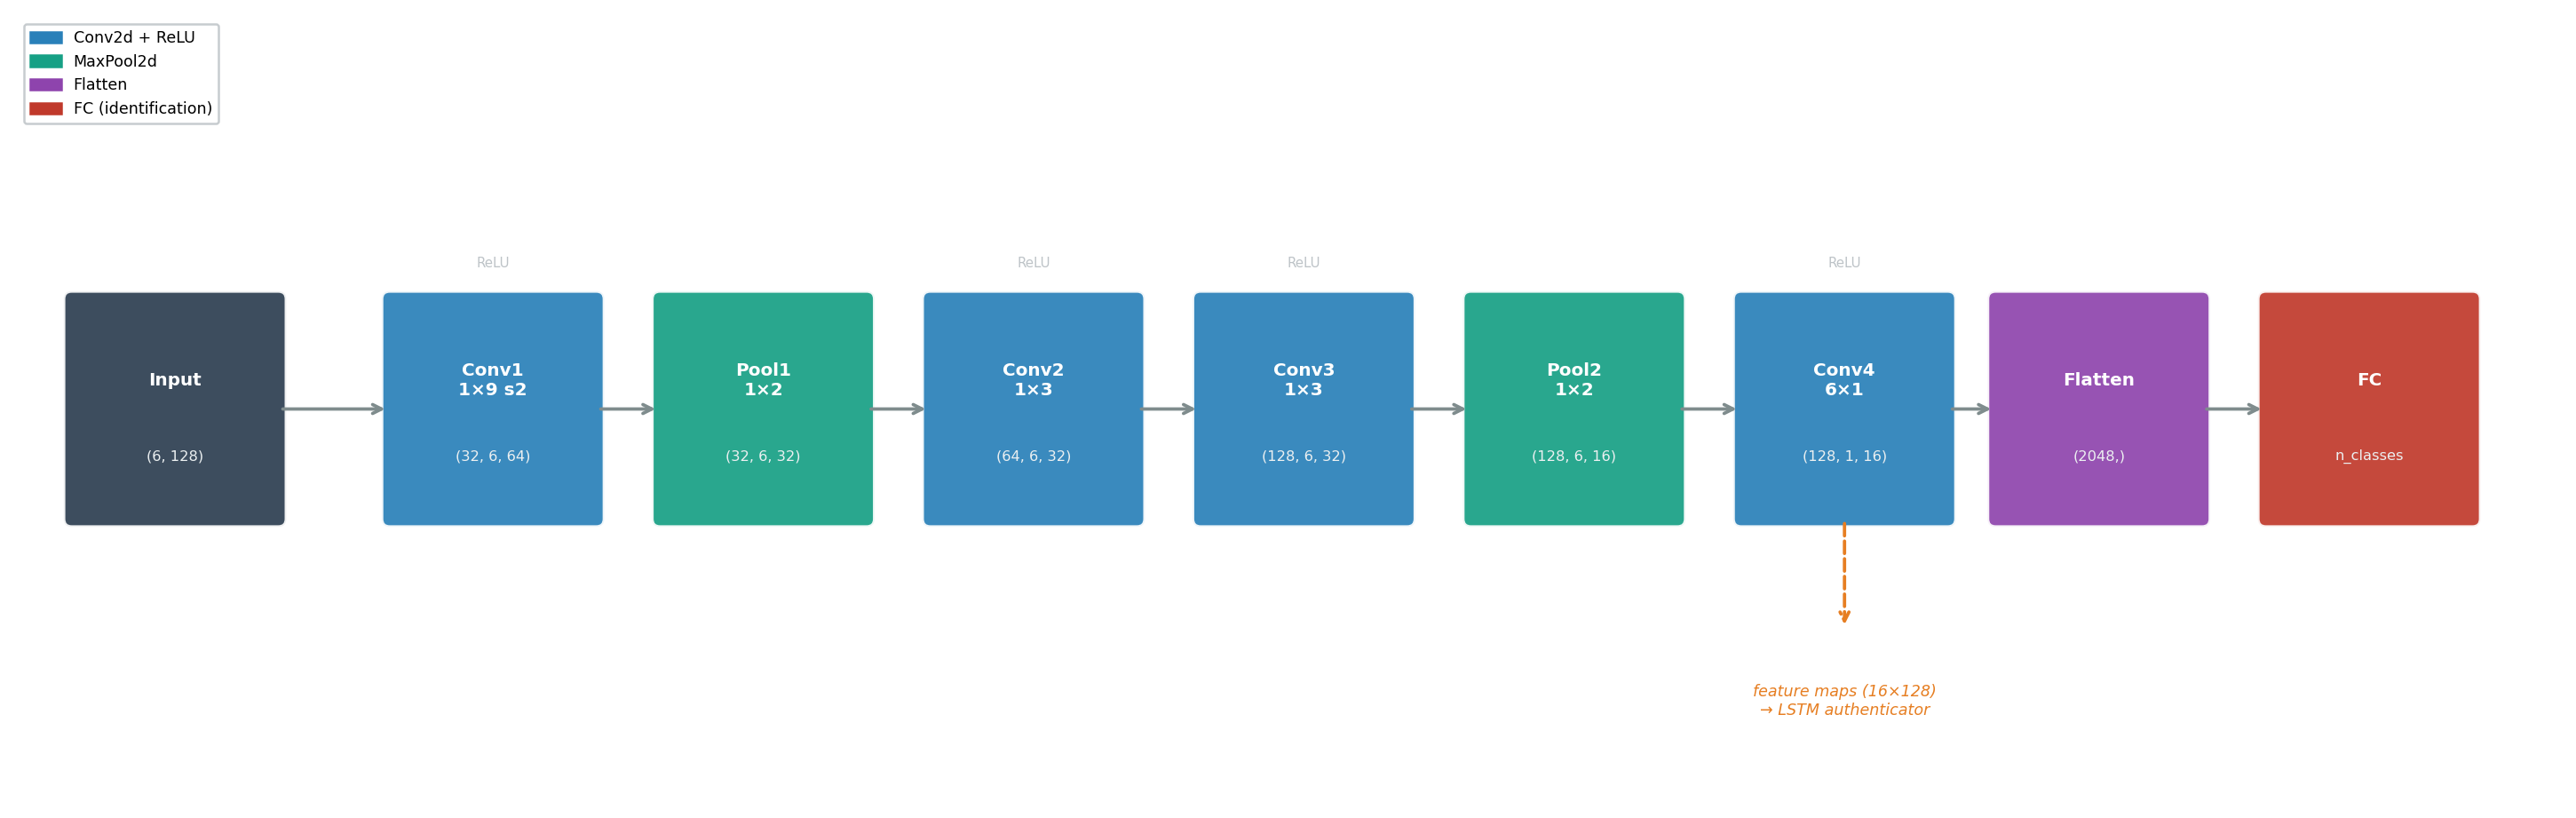
\includegraphics[width=\textwidth]{cnn_architecture.png}
  \caption{CNN encoder architecture (Zou et al.~\cite{zou2020deep}). Output
           shapes are shown below each block (batch dimension omitted). The
           dashed branch indicates the feature maps $(16, 128)$ passed to the
           LSTM authentication head; the main path continues to the FC layer
           used during identification pre-training.}
  \label{fig:cnn_arch}
\end{figure}

For identification pre-training the feature map is flattened to a 2048-dimensional vector and passed through a fully connected layer to produce logits over the $N$ training subjects. For the authentication head the flattening and FC layer are bypassed: the feature map is transposed to $(B, 16, 128)$ and fed directly to the LSTM.

\subsection{Training as Subject Identifier}
\label{ssec:sys_cnn_train}

For each within-dataset configuration the CNN is trained as a subject classifier on that dataset's member subjects, minimising cross-entropy loss on the per-window subject label. Training uses the Adam optimiser with a learning rate of $10^{-3}$, no weight decay, for 25 epochs with batch size 512. The CNN weights are fixed after identification training and are not updated during any subsequent stage.

% ─────────────────────────────────────────────────────────────────────────────
\section{Authentication Model}
\label{sec:sys_auth}

\subsection{LSTM Head and Similarity Score}
\label{ssec:sys_lstm}

The authentication model pairs the frozen CNN encoder with a trainable LSTM head, as shown in Figure~\ref{fig:auth_arch}. Both windows are encoded to $(16, 128)$ feature sequences, concatenated to $(32, 128)$, and processed by a 2-layer LSTM (hidden size 64). The last hidden state is projected through dropout and a fully connected layer to a score $P(\text{different person} \mid \mathbf{x}_1, \mathbf{x}_2) \in [0, 1]$; a pair is accepted as genuine if this score is below 0.5. The LSTM head has 83,074 trainable parameters.

\begin{figure}[htbp]
  \centering
  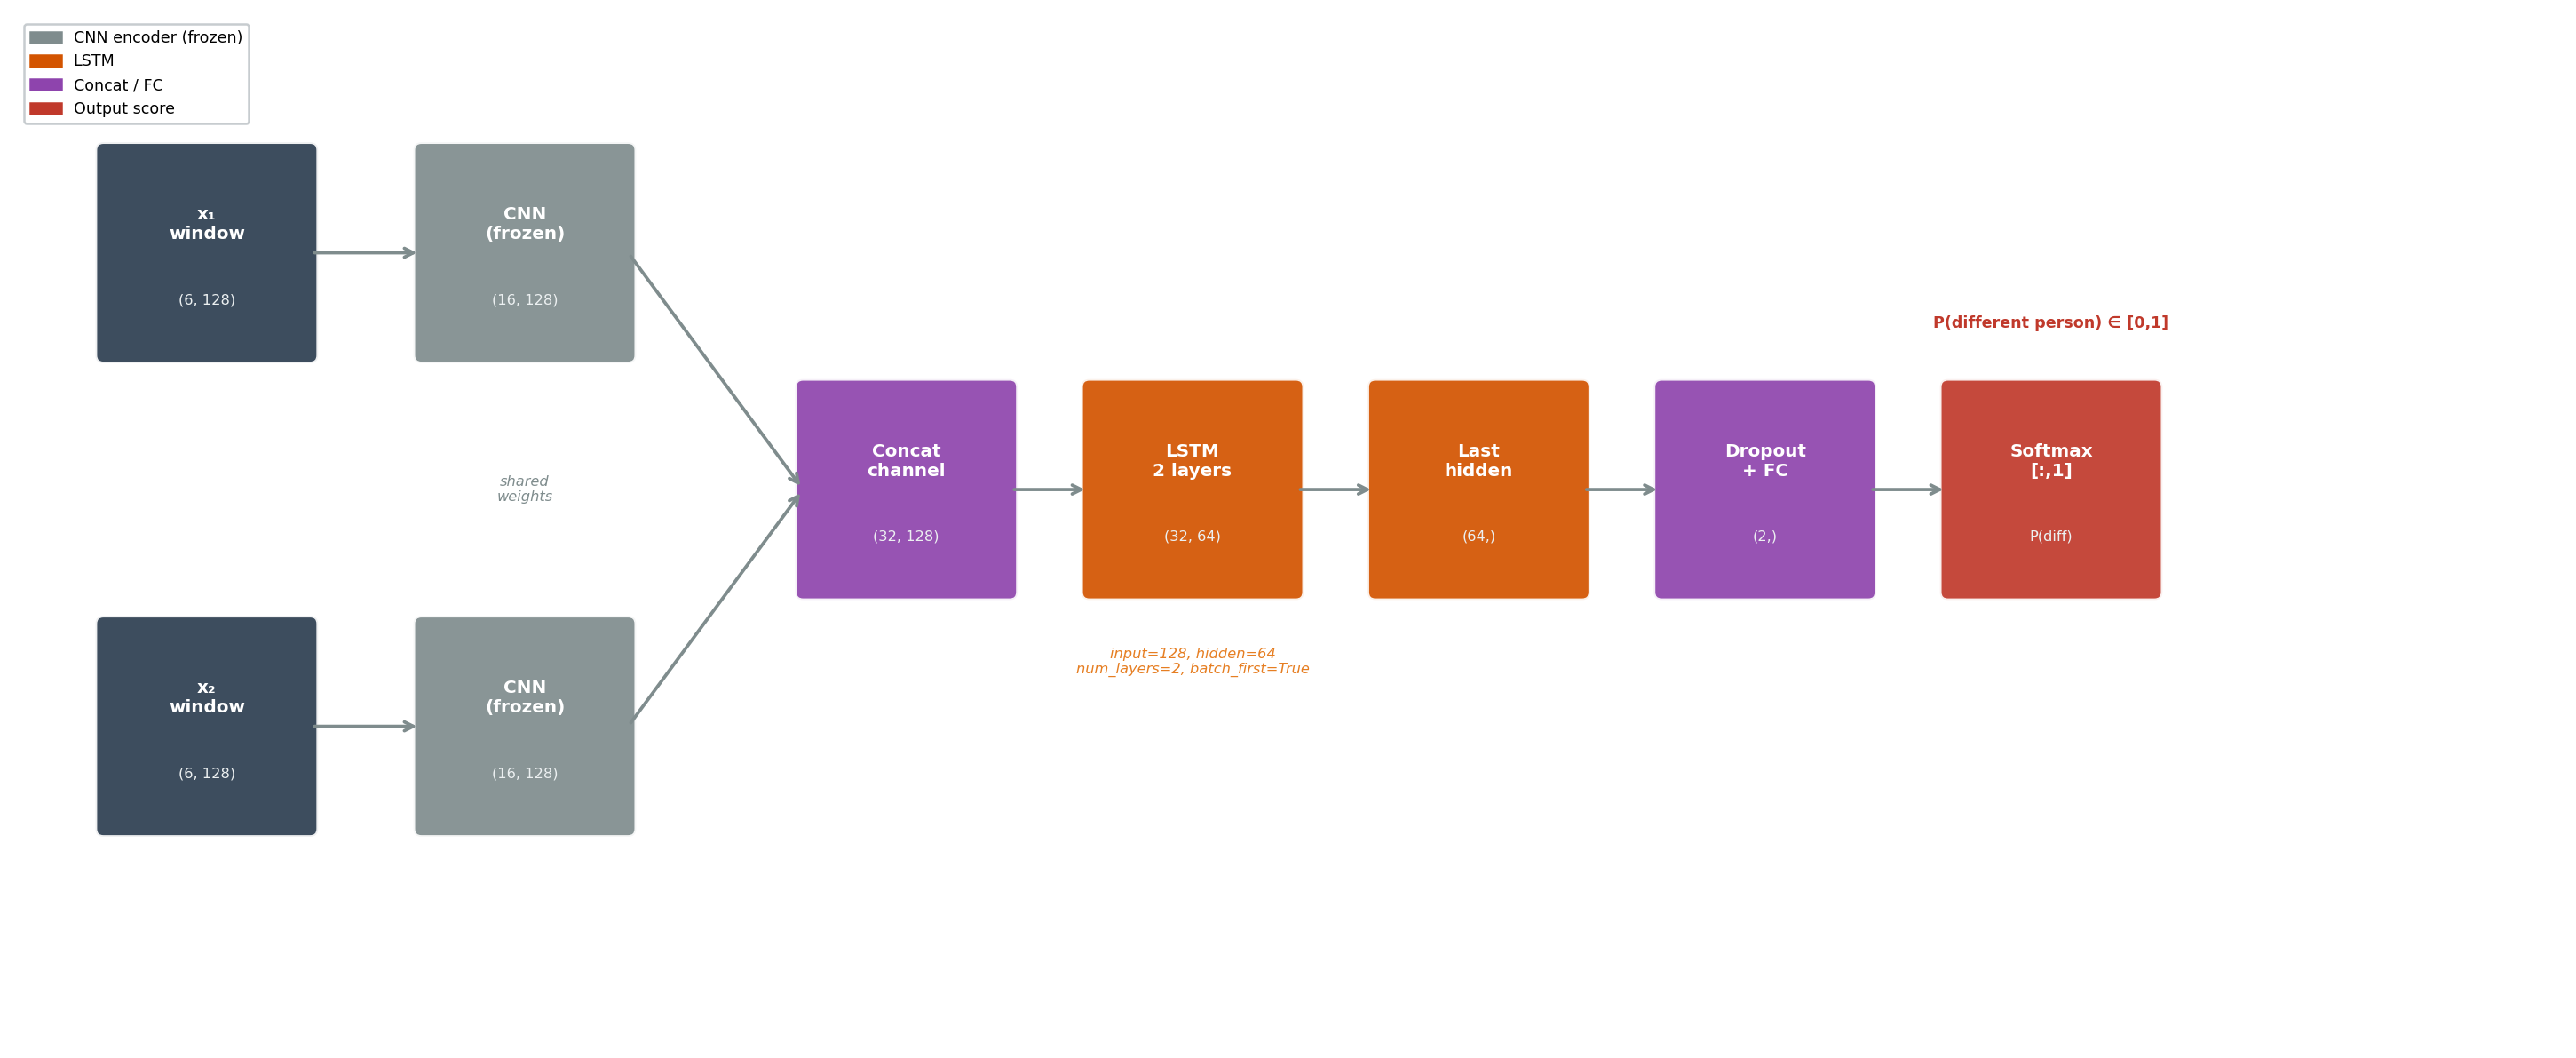
\includegraphics[width=\textwidth]{auth_architecture.png}
  \caption{AuthModel architecture. Both windows pass through the same frozen
           CNN encoder (weights shared). The resulting $(16,128)$ sequences
           are concatenated and fed to a 2-layer LSTM; the last hidden state
           is projected to a similarity score via dropout and a fully connected
           layer.}
  \label{fig:auth_arch}
\end{figure}

\subsection{Training Procedure}
\label{ssec:sys_auth_train}

The LSTM head is trained on the member pairs using the Adam optimiser with learning rate $2.5 \times 10^{-3}$, L2 weight decay $1.5 \times 10^{-3}$, batch size 512, and dropout rate 0.3. Training runs for 10 epochs. The CNN weights are frozen throughout; only the LSTM weights and the FC layer are updated. This keeps the two stages independent: the CNN is shaped by the identification objective, the LSTM by the pairwise comparison objective. The signal disentanglement experiment in Section~\ref{sec:mia_signal} exploits this separation to measure how much each component contributes to the membership signal.

Figure~\ref{fig:training_curves} shows the per-epoch train and test accuracy and loss for the authentication head across all four experimental configurations. The dotted vertical line marks the epoch selected by early stopping. whuGAIT trains for 2 epochs before the test accuracy stagnates; UCI-HAR and the combined run stop at epochs 2 and 8 respectively; WISDM trains for the full 10 epochs with the test accuracy still improving at the end. The growing train/test gap in UCI-HAR is consistent with the relatively small member pool (21 subjects), which gives the LSTM fewer pairs to generalise from.

Early stopping is monitored on the test (non-member) subjects, so the saved checkpoint is the one that generalises best to held-out identities. This is technically a form of evaluation contamination: the test population influences which model is retained. However, the bias runs in the conservative direction for membership inference. A model selected for good non-member generalisation is less overfit to its training subjects than one saved at peak training accuracy, which means the member--non-member delta gap is smaller and the MIA signal is weaker. The attack AUCs reported in subsequent chapters are therefore a lower bound: a model trained without test-set guidance would likely produce a stronger membership signal.

\begin{figure}[htbp]
  \centering
  \includegraphics[width=\textwidth]{analysis/models_overfitting_curves.png}
  \caption{Per-epoch train (solid) and test (dashed) accuracy and cross-entropy
           loss for the authentication head across all four configurations. The
           dotted vertical line marks the selected checkpoint epoch.}
  \label{fig:training_curves}
\end{figure}

% ─────────────────────────────────────────────────────────────────────────────
\section{Experimental Configurations}
\label{sec:sys_configs}

Five configurations are evaluated. The first four differ in which dataset the CNN and authentication head are trained on and which subjects form the held-out test set. The fifth is the signal disentanglement configuration, in which the CNN and LSTM are trained on disjoint subject groups within whuGAIT to isolate each component's contribution to the membership signal (Section~\ref{sec:mia_signal}).

\subsection{Within-Dataset Runs}
\label{ssec:sys_within}

The three within-dataset configurations each use a single dataset for all stages of the pipeline.

\textbf{whuGAIT.} The CNN is trained for identification on the 98 member subjects. The authentication head is then trained on pairs drawn from the same 98 subjects. The 20 non-member subjects serve as the held-out class for both the authentication evaluation and the MIA attack.

\textbf{UCI-HAR.} The CNN is trained from scratch on the 21 UCI-HAR member subjects for identification, then frozen. The authentication head is trained on pairs from the same 21 subjects. The 9 held-out subjects are the non-member class.

\textbf{WISDM.} The CNN is trained from scratch on the 40 WISDM member subjects for identification, then frozen. The authentication head is trained on pairs from the same 40 subjects, with 11 subjects held out.

\subsection{Cross-Dataset (Combined) Run}
\label{ssec:sys_combined}

The combined configuration assembles a training set from all three datasets: the 98 whuGAIT members, the 21 UCI-HAR members, and the 40 WISDM members, giving 159 training subjects in total. The whuGAIT CNN encoder is used and kept frozen. The authentication head is trained on pairs from all 159 subjects simultaneously. The resulting training inventory contains 72,000 pairs: 60,000 from whuGAIT and 6,000 each from UCI-HAR and WISDM. The imbalance reflects the larger subject count of whuGAIT, since pairs are sampled proportionally per subject.

The held-out test set consists of the 9 UCI-HAR non-members and the 11 WISDM non-members (20 subjects total), identified by a numeric offset that encodes their source dataset. No whuGAIT non-members are included in the combined test set, because the whuGAIT CNN was pre-trained on the whuGAIT members and the MIA signal for whuGAIT subjects is analysed separately in the within-dataset run.

\subsection{Signal Disentanglement Run}
\label{ssec:sys_signal}

The signal disentanglement configuration is a fifth pipeline run using 116 of the 118 available whuGAIT subjects, partitioned into four contiguous non-overlapping groups of 29:

\begin{itemize}
  \item \textbf{Group A (subjects 1--29):} CNN identification training only.
    The authentication head never sees pairs from these subjects.
  \item \textbf{Group B (subjects 30--58):} authentication head training only.
    The CNN is not trained to classify these subjects.
  \item \textbf{Group C (subjects 59--87):} held out from both training stages;
    serves as the non-member baseline for the MIA attack.
  \item \textbf{Group D (subjects 88--116):} used in both CNN identification
    training and authentication head training.
\end{itemize}

Each group has 29 subjects so that the CNN and the LSTM are trained on the same amount of data per component. Subjects 117--118 are unused. Group D tests whether the two memorisation signals combine super-additively: if the joint signal from D exceeds the maximum of A and B, the two components reinforce each other. The results are analysed in Section~\ref{sec:mia_signal}.

% ─────────────────────────────────────────────────────────────────────────────
\section{Authenticator Evaluation}
\label{sec:auth_eval}

Before examining attacks against the model, it is useful to characterise how the authentication model behaves across four distinct pair-type pools. The four pools are constructed from member subjects (enrolled during training, $\mathcal{M}$) and non-member subjects (held out, $\mathcal{N}$):

\begin{itemize}
  \item \textbf{MM}: probe and gallery both from $\mathcal{M}$; 50\% genuine, 50\% impostor.
  \item \textbf{NN}: probe and gallery both from $\mathcal{N}$; 50\% genuine, 50\% impostor.
  \item \textbf{MN}: probe from $\mathcal{M}$, gallery from $\mathcal{N}$; 100\% impostor.
  \item \textbf{NM}: probe from $\mathcal{N}$, gallery from $\mathcal{M}$; 100\% impostor.
\end{itemize}

The NN pool is the primary accuracy metric: it uses only held-out subjects and the balanced genuine/impostor split makes accuracy directly interpretable as the fraction of correctly classified pairs. The MM pool measures in-distribution performance. The MN and NM pools are all-impostor; their accuracy is the true rejection rate for cross-membership pairs.

Table~\ref{tab:four_case} reports accuracy and AUC for MM and NN across the three within-dataset configurations. The AUC gap (MM $-$ NN) indicates how much more discriminatively the model handles its training subjects compared to held-out subjects.

\begin{table}[htbp]
\centering
\caption{Four-case authenticator evaluation. MM and NN use balanced genuine/impostor pairs; MN and NM are all-impostor (accuracy $=$ true rejection rate). NN accuracy is the held-out generalisation metric.}
\label{tab:four_case}
\begin{tabular}{lrrrrrr}
\toprule
Dataset & MM acc & MM AUC & NN acc & NN AUC & MN acc & NM acc \\
\midrule
whuGAIT & \whugaitFourCaseMMAcc & \whugaitFourCaseMMAuc & \whugaitFourCaseNNAcc & \whugaitFourCaseNNAuc & \whugaitFourCaseMNAcc & \whugaitFourCaseNMAcc \\
UCI-HAR & \uciharFourCaseMMAcc  & \uciharFourCaseMMAuc  & \uciharFourCaseNNAcc  & \uciharFourCaseNNAuc  & \uciharFourCaseMNAcc  & \uciharFourCaseNMAcc  \\
WISDM   & \wisdmFourCaseMMAcc   & \wisdmFourCaseMMAuc   & \wisdmFourCaseNNAcc   & \wisdmFourCaseNNAuc   & \wisdmFourCaseMNAcc   & \wisdmFourCaseNMAcc   \\
\bottomrule
\end{tabular}
\end{table}

The MM--NN AUC gap (MM AUC minus NN AUC) quantifies how much more discriminatively the model handles its training subjects relative to held-out ones. A positive gap indicates that the LSTM has fitted training pairs more tightly than it generalises to unseen subjects: members produce higher, more consistent deltas, while non-members produce a weaker, noisier response. This asymmetry is the structural prerequisite for the attacks in Chapters~\ref{ch:evasion} and~\ref{ch:mia}: where the gap is larger, the attack has a stronger signal to exploit; where it approaches zero, the model generalises comparably to both populations and the membership signal weakens. All configurations show a positive gap, confirming that overfitting to training subjects is a consistent property of the pipeline across datasets.

\begin{figure}[htbp]
  \centering
  \includegraphics[width=0.85\textwidth]{analysis/models_four_case_summary.png}
  \caption{Four-case accuracy (MM, NN, MN, NM) and MM vs.\ NN AUC across the three within-dataset configurations. The AUC gap between MM and NN quantifies how much more discriminatively the model handles enrolled subjects.}
  \label{fig:four_case_summary}
\end{figure}

\begin{figure}[htbp]
  \centering
  \begin{subfigure}[b]{0.48\textwidth}
    \includegraphics[width=\textwidth]{analysis/models_four_case_whuGAIT.png}
    \caption{whuGAIT}
  \end{subfigure}
  \hfill
  \begin{subfigure}[b]{0.48\textwidth}
    \includegraphics[width=\textwidth]{analysis/models_four_case_ucihar.png}
    \caption{UCI-HAR}
  \end{subfigure}
  \vspace{0.5em}
  \begin{subfigure}[b]{0.48\textwidth}
    \includegraphics[width=\textwidth]{analysis/models_four_case_wisdm.png}
    \caption{WISDM}
  \end{subfigure}
  \hfill
  \begin{subfigure}[b]{0.48\textwidth}
    \includegraphics[width=\textwidth]{analysis/models_four_case_combined.png}
    \caption{Combined}
  \end{subfigure}
  \caption{Score distributions across the four pair-type pools for all configurations. The separation between MM and NN genuine/impostor distributions is tighter for enrolled subjects than for held-out ones, consistent with the accuracy gaps in Table~\ref{tab:four_case}. The Combined configuration shows the weakest separation, reflecting the cross-dataset distribution shift.}
  \label{fig:four_case_detail}
\end{figure}
\chapter{Evasion Attack}
\label{ch:evasion}

This chapter analyses whether the authentication model's decision boundary is robust: given an impostor pair that the model correctly rejects, how much does the probe signal need to change before the model accepts it? A perturbation $\boldsymbol{\delta}$ is added to the probe window and optimised via PGD to push the model's output below the acceptance threshold. The experiment is run over the impostor pairs in the test set, so the result quantifies how close the boundary is to naturally occurring gait signals across the subject population, rather than for a single targeted case. The perturbation budget is calibrated against the natural trial-to-trial variability of the signal, giving a reference scale for whether the required change is within or beyond what the model should already tolerate as normal intra-subject variation. The minimum effective perturbation budget $\varepsilon_\text{min}$ established here is later used as a membership inference signal in Chapter~\ref{ch:mia}.

% ─────────────────────────────────────────────────────────────────────────────
\section{Attack Formulation}
\label{sec:ev_formulation}

\subsection{False Accept Objective}
\label{ssec:ev_objective}

The attack targets impostor pairs: two windows from different subjects that the authentication model would correctly reject. The attacker controls the probe window $\mathbf{x}_1$ and adds a perturbation $\boldsymbol{\delta}$ before it reaches the model. The reference window $\mathbf{x}_2$ stored in the authentication database is untouched. The goal is not to mimic a specific subject's gait but to push the model's output score across the decision boundary.

The attack succeeds when the perturbed pair is accepted:
\begin{equation}
  P\!\left(\text{different person} \mid \mathbf{x}_1 + \boldsymbol{\delta},\,
  \mathbf{x}_2\right) < 0.5.
\end{equation}
The attack surface is the raw sensor signal: the 6-channel, 128-timestep IMU window. The CNN and LSTM are not modified; the gradient flows through both during optimisation.

\subsection{Norm Choice and Optimisation}
\label{ssec:ev_pgd}

The $\ell_2$ norm is chosen over $\ell_\infty$ for both physical and empirical reasons. A natural change in human gait distributes energy continuously across all sensor channels and all timesteps: a slightly longer stride or a shift in arm swing affects the full window, not a handful of isolated samples. An $\ell_\infty$ constraint allows the perturbation to concentrate its entire budget into a few large spikes at individual sensor readings, which correspond to sharp impact events that are physically implausible and easy to detect. An $\ell_2$ constraint instead bounds the total perturbation energy and encourages smooth, broadband changes that more closely resemble natural intra-subject variation. This choice also connects directly to the budget calibration: $\varepsilon_\text{target}$ is itself an $\ell_2$ distance (Section~\ref{sec:ev_budget}), making the budget ratio $\varepsilon_\text{min}/\varepsilon_\text{target}$ directly interpretable.

The perturbation is found by standard PGD~\cite{madry2018towards}: starting from the clean probe $\mathbf{x}_1$, each of $K$ steps takes a gradient step on the cross-entropy loss with target label 0 (same person) and projects the result back onto the $\ell_2$ ball of radius $\varepsilon$. All experiments use $K = 20$ iterations, confirmed sufficient by the ablation in Section~\ref{ssec:ev_spectral_k}.

% ─────────────────────────────────────────────────────────────────────────────
\section{Perturbation Budget Estimation}
\label{sec:ev_budget}

\subsection{Intra-Subject L2 as Reference Scale}
\label{ssec:ev_l2}

Rather than fixing $\varepsilon$ arbitrarily, the budget is anchored to the natural variability of the signal being attacked. For each dataset, $\varepsilon_\text{target}$ is defined as the median $\ell_2$ distance between two windows recorded from the same subject in the training split:
\begin{equation}
  \varepsilon_\text{target}
  = \mathrm{median}_{(i,j)\,:\,s_i = s_j}
    \left\| \mathbf{x}_i - \mathbf{x}_j \right\|_2.
\end{equation}
A perturbation with $\|\boldsymbol{\delta}\|_2 \leq \varepsilon_\text{target}$ is smaller than the typical difference between two windows from the same person, giving a reference point for what the model should already tolerate as natural intra-subject variation.

The resulting values are $\varepsilon_\text{target} = \whuGAITEpsTarget$ (whuGAIT), $\uciharEpsTarget$ (UCI-HAR), $\wisdmEpsTarget$ (WISDM), and $\combinedEpsTarget$ (combined). The differences reflect window length and sampling rate: WISDM's 20\,Hz, 128-sample windows span 6.4 seconds and accumulate more cycle-to-cycle variation than shorter windows.

\subsection{Grid Sweep and Binary Search}
\label{ssec:ev_grid}

For each impostor pair $(A, B)$ the minimum effective budget $\varepsilon_\text{min}$ is found in two phases. First, a geometric grid of $\varepsilon$ values spanning $[5\%\,\varepsilon_\text{target},\,
\varepsilon_\text{target}]$ plus sparse sentinels at $2\times$, $5\times$, and
$10\times \varepsilon_\text{target}$ is swept in ascending order. A pair exits the sweep at the first $\varepsilon$ where the PGD attack succeeds, defining a bracket $[\varepsilon_\text{lo}, \varepsilon_\text{hi}]$. Pairs that do not succeed even at the $10\times$ sentinel are classified as resistant.

Second, $N_\text{bisect} = 10$ binary search steps narrow the bracket to a refined $\varepsilon_\text{min} \approx \varepsilon_\text{hi}$, which is the smallest confirmed successful budget for that pair.

Figure~\ref{fig:evasion_eps} shows the resulting distribution of per-pair normalised budgets across all four dataset configurations. Most pairs are broken well below $\varepsilon_\text{target}$, with the bulk of the mass below 1.

\begin{figure}[htbp]
  \centering
  \includegraphics[width=\textwidth]{analysis/evasion_eps_distribution.png}
  \caption{Distribution of normalised minimum attack budget
           $\varepsilon_\text{min}/\varepsilon_\text{target}$ over succeeded
           test-split pairs. The dashed vertical line marks $\varepsilon_\text{target}$
           (budget ratio $= 1$); the red line shows the mean.}
  \label{fig:evasion_eps}
\end{figure}

% ─────────────────────────────────────────────────────────────────────────────
\section{Results}
\label{sec:ev_results}

\subsection{Test-Split Attack}
\label{ssec:ev_asr}

The test split contains impostor pairs formed from non-member subjects the model has never seen during training. Table~\ref{tab:evasion_results} reports the combo-level ASR and mean budget ratio $\varepsilon_\text{min}/\varepsilon_\text{target}$ for all four dataset configurations.

\begin{table}[htbp]
\centering
\caption{Evasion attack on the test split (non-member pairs). Budget ratio is the mean
         $\varepsilon_\text{min} / \varepsilon_\text{target}$ over successful pairs.}
\label{tab:evasion_results}
\begin{tabular}{lrrrr}
\toprule
Dataset  & $\varepsilon_\text{target}$ & Combos & ASR & Budget ratio \\
\midrule
whuGAIT  & \whuGAITEpsTarget  & \whuGAITNCombos  & \whuGAITComboASR  & \whuGAITBudgetRatio  \\
UCI-HAR  & \uciharEpsTarget   & \uciharNCombos   & \uciharComboASR   & \uciharBudgetRatio   \\
WISDM    & \wisdmEpsTarget    & \wisdmNCombos    & \wisdmComboASR    & \wisdmBudgetRatio    \\
Combined & \combinedEpsTarget & \combinedNCombos & \combinedComboASR & \combinedBudgetRatio \\
\bottomrule
\end{tabular}
\end{table}

The attack succeeds on the majority of pairs. whuGAIT achieves an ASR of \whuGAITComboASR{} with a median budget of \whuGAITBudgetRatio{} of $\varepsilon_\text{target}$: the required perturbation is a small fraction of the natural intra-subject spread. WISDM requires a larger relative budget (\wisdmBudgetRatio{} of $\varepsilon_\text{target}$), consistent with its longer windows capturing more person-specific cycle structure.

\subsection{Training-Split Attack}
\label{ssec:ev_traintest}

The training split contains impostor pairs formed from enrolled members. The model has calibrated its decision boundary directly on these subjects, so their genuine scores sit lower and require a larger perturbation to cross the threshold. Table~\ref{tab:evasion_train} shows the result.

\begin{table}[htbp]
\centering
\caption{Evasion attack on the training split (enrolled members). Budget
         ratio is mean $\varepsilon_\text{min} / \varepsilon_\text{target}$ over successful pairs.}
\label{tab:evasion_train}
\begin{tabular}{lrrr}
\toprule
Dataset  & $\varepsilon_\text{target}$ & ASR & Budget ratio \\
\midrule
whuGAIT  & \whuGAITEpsTarget  & \whuGAITTrainComboASR  & \whuGAITTrainBudgetRatio  \\
UCI-HAR  & \uciharEpsTarget   & \uciharTrainComboASR   & \uciharTrainBudgetRatio   \\
WISDM    & \wisdmEpsTarget    & \wisdmTrainComboASR    & \wisdmTrainBudgetRatio    \\
Combined & \combinedEpsTarget & \combinedTrainComboASR & \combinedTrainBudgetRatio \\
\bottomrule
\end{tabular}
\end{table}

The budget ratio is roughly $3$--$4\times$ larger on the training split than on the test split. Figure~\ref{fig:evasion_train_vs_test} shows the distribution shift.

\begin{figure}[htbp]
  \centering
  \includegraphics[width=\textwidth]{analysis/evasion_train_vs_test.png}
  \caption{Budget ratio distributions: training split (enrolled members, solid) vs.\ test split (held-out non-members, dashed). The training-split distribution is shifted right.}
  \label{fig:evasion_train_vs_test}
\end{figure}

\subsection{Four-Case Attack Breakdown}
\label{ssec:ev_fourcase}

Tables~\ref{tab:evasion_fourcase_whugait}--\ref{tab:evasion_fourcase_combined} report ASR and mean $\varepsilon_\text{min}$ per pair type and dataset configuration.

% Auto-generated by compare_evasion_fourcase_whuGAIT: DO NOT EDIT MANUALLY
% Last run: 2026-09-25 13:50:19

\providecommand{\pgdCaseMMAsr}{}
\renewcommand{\pgdCaseMMAsr}{0.999}
\providecommand{\pgdCaseMMMeanEps}{}
\renewcommand{\pgdCaseMMMeanEps}{6.7781}
\providecommand{\pgdCaseMMNPairs}{}
\renewcommand{\pgdCaseMMNPairs}{1649}
\providecommand{\pgdCaseNNAsr}{}
\renewcommand{\pgdCaseNNAsr}{0.999}
\providecommand{\pgdCaseNNMeanEps}{}
\renewcommand{\pgdCaseNNMeanEps}{4.7326}
\providecommand{\pgdCaseNNNPairs}{}
\renewcommand{\pgdCaseNNNPairs}{5000}
\providecommand{\pgdCaseNMAsr}{}
\renewcommand{\pgdCaseNMAsr}{0.999}
\providecommand{\pgdCaseNMMeanEps}{}
\renewcommand{\pgdCaseNMMeanEps}{4.6528}
\providecommand{\pgdCaseNMNPairs}{}
\renewcommand{\pgdCaseNMNPairs}{1000}
\providecommand{\pgdCaseMNAsr}{}
\renewcommand{\pgdCaseMNAsr}{1.000}
\providecommand{\pgdCaseMNMeanEps}{}
\renewcommand{\pgdCaseMNMeanEps}{5.2737}
\providecommand{\pgdCaseMNNPairs}{}
\renewcommand{\pgdCaseMNNPairs}{1000}

\begin{table}[htbp]
\centering
\caption{PGD evasion results by pair type: whuGAIT. MM: training split. NN, MN, NM: test split. Mean $\varepsilon_\text{min}$ is the mean per-combo minimum budget in raw sensor units.}
\label{tab:evasion_fourcase_whugait}
\begin{tabular}{lrrr}
\toprule
Pair type & N pairs & ASR & Mean $\varepsilon_\text{min}$ \\
\midrule
MM & \pgdCaseMMNPairs & \pgdCaseMMAsr & \pgdCaseMMMeanEps \\
NN & \pgdCaseNNNPairs & \pgdCaseNNAsr & \pgdCaseNNMeanEps \\
MN & \pgdCaseMNNPairs & \pgdCaseMNAsr & \pgdCaseMNMeanEps \\
NM & \pgdCaseNMNPairs & \pgdCaseNMAsr & \pgdCaseNMMeanEps \\
\bottomrule
\end{tabular}
\end{table}

% Auto-generated by compare_evasion_fourcase_ucihar: DO NOT EDIT MANUALLY
% Last run: 2026-09-25 13:50:19

\providecommand{\pgdCaseMMAsr}{}
\renewcommand{\pgdCaseMMAsr}{0.992}
\providecommand{\pgdCaseMMMeanEps}{}
\renewcommand{\pgdCaseMMMeanEps}{11.3261}
\providecommand{\pgdCaseMMNPairs}{}
\renewcommand{\pgdCaseMMNPairs}{30000}
\providecommand{\pgdCaseNNAsr}{}
\renewcommand{\pgdCaseNNAsr}{0.995}
\providecommand{\pgdCaseNNMeanEps}{}
\renewcommand{\pgdCaseNNMeanEps}{7.0693}
\providecommand{\pgdCaseNNNPairs}{}
\renewcommand{\pgdCaseNNNPairs}{5000}
\providecommand{\pgdCaseNMAsr}{}
\renewcommand{\pgdCaseNMAsr}{0.994}
\providecommand{\pgdCaseNMMeanEps}{}
\renewcommand{\pgdCaseNMMeanEps}{6.8219}
\providecommand{\pgdCaseNMNPairs}{}
\renewcommand{\pgdCaseNMNPairs}{945}
\providecommand{\pgdCaseMNAsr}{}
\renewcommand{\pgdCaseMNAsr}{0.989}
\providecommand{\pgdCaseMNMeanEps}{}
\renewcommand{\pgdCaseMNMeanEps}{9.3192}
\providecommand{\pgdCaseMNNPairs}{}
\renewcommand{\pgdCaseMNNPairs}{945}

\begin{table}[htbp]
\centering
\caption{PGD evasion results by pair type: UCI-HAR. MM: training split. NN, MN, NM: test split. Mean $\varepsilon_\text{min}$ in raw sensor units.}
\label{tab:evasion_fourcase_ucihar}
\begin{tabular}{lrrr}
\toprule
Pair type & N pairs & ASR & Mean $\varepsilon_\text{min}$ \\
\midrule
MM & \pgdCaseMMNPairs & \pgdCaseMMAsr & \pgdCaseMMMeanEps \\
NN & \pgdCaseNNNPairs & \pgdCaseNNAsr & \pgdCaseNNMeanEps \\
MN & \pgdCaseMNNPairs & \pgdCaseMNAsr & \pgdCaseMNMeanEps \\
NM & \pgdCaseNMNPairs & \pgdCaseNMAsr & \pgdCaseNMMeanEps \\
\bottomrule
\end{tabular}
\end{table}

% Auto-generated by compare_evasion_fourcase_wisdm: DO NOT EDIT MANUALLY
% Last run: 2026-09-25 13:50:19

\providecommand{\pgdCaseMMAsr}{}
\renewcommand{\pgdCaseMMAsr}{0.962}
\providecommand{\pgdCaseMMMeanEps}{}
\renewcommand{\pgdCaseMMMeanEps}{27.4070}
\providecommand{\pgdCaseMMNPairs}{}
\renewcommand{\pgdCaseMMNPairs}{9579}
\providecommand{\pgdCaseNNAsr}{}
\renewcommand{\pgdCaseNNAsr}{0.979}
\providecommand{\pgdCaseNNMeanEps}{}
\renewcommand{\pgdCaseNNMeanEps}{28.9132}
\providecommand{\pgdCaseNNNPairs}{}
\renewcommand{\pgdCaseNNNPairs}{5000}
\providecommand{\pgdCaseNMAsr}{}
\renewcommand{\pgdCaseNMAsr}{0.971}
\providecommand{\pgdCaseNMMeanEps}{}
\renewcommand{\pgdCaseNMMeanEps}{27.7687}
\providecommand{\pgdCaseNMNPairs}{}
\renewcommand{\pgdCaseNMNPairs}{1000}
\providecommand{\pgdCaseMNAsr}{}
\renewcommand{\pgdCaseMNAsr}{0.982}
\providecommand{\pgdCaseMNMeanEps}{}
\renewcommand{\pgdCaseMNMeanEps}{26.7177}
\providecommand{\pgdCaseMNNPairs}{}
\renewcommand{\pgdCaseMNNPairs}{1000}

\begin{table}[htbp]
\centering
\caption{PGD evasion results by pair type: WISDM. MM: training split. NN, MN, NM: test split. Mean $\varepsilon_\text{min}$ in raw sensor units.}
\label{tab:evasion_fourcase_wisdm}
\begin{tabular}{lrrr}
\toprule
Pair type & N pairs & ASR & Mean $\varepsilon_\text{min}$ \\
\midrule
MM & \pgdCaseMMNPairs & \pgdCaseMMAsr & \pgdCaseMMMeanEps \\
NN & \pgdCaseNNNPairs & \pgdCaseNNAsr & \pgdCaseNNMeanEps \\
MN & \pgdCaseMNNPairs & \pgdCaseMNAsr & \pgdCaseMNMeanEps \\
NM & \pgdCaseNMNPairs & \pgdCaseNMAsr & \pgdCaseNMMeanEps \\
\bottomrule
\end{tabular}
\end{table}

% Auto-generated by compare_evasion_fourcase_combined: DO NOT EDIT MANUALLY
% Last run: 2026-09-25 13:50:19

\providecommand{\pgdCaseMMAsr}{}
\renewcommand{\pgdCaseMMAsr}{0.998}
\providecommand{\pgdCaseMMMeanEps}{}
\renewcommand{\pgdCaseMMMeanEps}{8.9916}
\providecommand{\pgdCaseMMNPairs}{}
\renewcommand{\pgdCaseMMNPairs}{1690}
\providecommand{\pgdCaseNNAsr}{}
\renewcommand{\pgdCaseNNAsr}{0.992}
\providecommand{\pgdCaseNNMeanEps}{}
\renewcommand{\pgdCaseNNMeanEps}{6.3338}
\providecommand{\pgdCaseNNNPairs}{}
\renewcommand{\pgdCaseNNNPairs}{6000}
\providecommand{\pgdCaseNMAsr}{}
\renewcommand{\pgdCaseNMAsr}{0.990}
\providecommand{\pgdCaseNMMeanEps}{}
\renewcommand{\pgdCaseNMMeanEps}{8.6438}
\providecommand{\pgdCaseNMNPairs}{}
\renewcommand{\pgdCaseNMNPairs}{1000}
\providecommand{\pgdCaseMNAsr}{}
\renewcommand{\pgdCaseMNAsr}{0.998}
\providecommand{\pgdCaseMNMeanEps}{}
\renewcommand{\pgdCaseMNMeanEps}{7.3719}
\providecommand{\pgdCaseMNNPairs}{}
\renewcommand{\pgdCaseMNNPairs}{1000}

\begin{table}[htbp]
\centering
\caption{PGD evasion results by pair type: Combined. MM: training split. NN, MN, NM: test split. Mean $\varepsilon_\text{min}$ in raw sensor units.}
\label{tab:evasion_fourcase_combined}
\begin{tabular}{lrrr}
\toprule
Pair type & N pairs & ASR & Mean $\varepsilon_\text{min}$ \\
\midrule
MM & \pgdCaseMMNPairs & \pgdCaseMMAsr & \pgdCaseMMMeanEps \\
NN & \pgdCaseNNNPairs & \pgdCaseNNAsr & \pgdCaseNNMeanEps \\
MN & \pgdCaseMNNPairs & \pgdCaseMNAsr & \pgdCaseMNMeanEps \\
NM & \pgdCaseNMNPairs & \pgdCaseNMAsr & \pgdCaseNMMeanEps \\
\bottomrule
\end{tabular}
\end{table}

The expected pattern is that MM requires a larger mean $\varepsilon_\text{min}$ than NN: enrolled subjects have tighter genuine/impostor separation (Section~\ref{sec:auth_eval}), so a perturbation must bridge a wider gap to reach the acceptance threshold. WISDM is the exception, where all four pools cluster near $\varepsilon_\text{target}$ with minimal differences between pair types; this is consistent with WISDM's stronger model generalisation (small MM--NN AUC gap in Table~\ref{tab:four_case}), which leaves little asymmetry for the budget to reflect.

Where MM requires a larger budget than NN, that asymmetry is a candidate membership inference signal: a probe subject whose pairs demand more perturbation is likely enrolled. Chapter~\ref{ch:mia} evaluates this signal formally, pooling all four pair types per probe subject.

A note on aggregation: the budget ratio in Tables~\ref{tab:evasion_results} and~\ref{tab:evasion_train} is the pair-level mean $\varepsilon_\text{min}/\varepsilon_\text{target}$, while the mean $\varepsilon_\text{min}$ here is the combo-level mean. The two statistics agree in direction but differ in magnitude.

The group-level means, however, mask high within-group variance. Each subject's mean $\varepsilon_\text{min}$ is computed from a limited number of pairs and reflects not just membership but also that subject's intrinsic gait distinctiveness: a subject with a highly idiosyncratic gait is hard to impersonate regardless of enrolment status. This per-subject noise limits discrimination to AUC $\approx 0.58$ on whuGAIT and AUC $\approx 0.67$ on UCI-HAR despite the clear group-level difference.

On WISDM the problem is compounded: all four cases cluster near $\varepsilon_\text{target}$ (budget ratios 0.86--0.93), meaning the attack is uniformly difficult across all subjects. There is almost no residual spread to discriminate on, and the marginal inversion (member mean $27.4$ vs non-member mean $28.9$) makes the per-subject AUC fall below 0.5.

\subsection{Feature-Space Analysis}
\label{ssec:ev_features}

The attack optimises the input end-to-end through both the CNN and the LSTM, but this does not indicate which component is being exploited. Figure~\ref{fig:feature_shift} shows the CNN embedding distance before and after perturbation on 200 sampled whuGAIT pairs. The scatter plot reveals that adversarial distances are nearly identical to clean distances — points lie on the diagonal — and the ratio histogram is sharply concentrated at 1.0 (mean ratio 1.006). The attack does not substantially close the CNN representation gap between the two subjects; instead it exploits the LSTM's decision boundary directly, producing an input that the classifier accepts without materially altering the CNN embedding. The same pattern holds across all dataset configurations.

\begin{figure}[htbp]
  \centering
  \includegraphics[width=\textwidth]{whuGAIT/06c_whuGAIT_feature_shift.png}
  \caption{CNN feature-space shift on 200 sampled whuGAIT pairs. Left: adversarial
           vs.\ clean embedding distance between the two subjects; points on the
           diagonal indicate no change. Right: distribution of the distance ratio
           $d_\text{adv}/d_\text{clean}$; the mean of 1.006 shows the perturbation
           does not close the representation gap. The attack exploits the LSTM
           decision boundary rather than aligning CNN embeddings.}
  \label{fig:feature_shift}
\end{figure}

% Auto-generated by nb06c_whuGAIT: DO NOT EDIT MANUALLY
% Last run: 2026-09-24 17:53:16

\providecommand{\spectralFracInBand}{}
\renewcommand{\spectralFracInBand}{67.7}
\providecommand{\spectralFCutoff}{}
\renewcommand{\spectralFCutoff}{10}
\providecommand{\detectionPValue}{}
\renewcommand{\detectionPValue}{0.4284}
\providecommand{\detectionDistinguish}{}
\renewcommand{\detectionDistinguish}{no}
\providecommand{\hfrCleanMean}{}
\renewcommand{\hfrCleanMean}{0.0980}
\providecommand{\hfrAdvMean}{}
\renewcommand{\hfrAdvMean}{0.1019}
\providecommand{\kValues}{}
\renewcommand{\kValues}{[5, 10, 20, 40, 80]}
\providecommand{\kOriginal}{}
\renewcommand{\kOriginal}{20}
\providecommand{\kConvergenceRatio}{}
\renewcommand{\kConvergenceRatio}{0.244}
\providecommand{\kBestEps}{}
\renewcommand{\kBestEps}{80}
\providecommand{\kBestMeanEpsMin}{}
\renewcommand{\kBestMeanEpsMin}{3.4221}
\providecommand{\featureCloserFrac}{}
\renewcommand{\featureCloserFrac}{62.5}
\providecommand{\featureMeanRatio}{}
\renewcommand{\featureMeanRatio}{1.006}
\providecommand{\nSampleSpectral}{}
\renewcommand{\nSampleSpectral}{200}
\providecommand{\nSampleAblation}{}
\renewcommand{\nSampleAblation}{100}

% ─────────────────────────────────────────────────────────────────────────────
\section{Spectral Analysis and Detection Resistance}
\label{sec:ev_spectral}

\subsection{Frequency Distribution of Perturbations}
\label{ssec:ev_spectral_freq}

A perturbation small in $\ell_2$ could still be detectable if its energy concentrates at frequencies outside the biological range of human gait. Human gait produces most IMU signal energy below 10\,Hz (stride frequency and harmonics); above that band the signal decays toward the sensor noise floor.

Figure~\ref{fig:spectral_psd} shows the mean PSD for whuGAIT. In the gait band the perturbation (green dotted) sits well below both clean and adversarial signals, which are nearly indistinguishable. Above $\sim$20\,Hz, where the clean gait signal has already decayed to negligible absolute power, the perturbation decays more slowly and the adversarial signal locally exceeds the clean in the accelerometer channels; the gyroscope channels do not show this effect. This high-frequency excess is real but small in absolute terms: most perturbation energy falls in the 0--10\,Hz gait band, and a Mann-Whitney test on the fraction of total signal energy above 10\,Hz finds no significant difference between clean and adversarial groups. A spectral detector operating on the energy fraction above 10\,Hz would not flag these examples; a detector specifically targeting the 20--25\,Hz tail could in principle detect the excess, but would need to be calibrated against naturally occurring gait noise at those frequencies.

\begin{figure}[htbp]
  \centering
  \includegraphics[width=\textwidth]{whuGAIT/06c_whuGAIT_spectral.png}
  \caption{Mean PSD (log scale) of clean (blue solid), adversarial (red dashed),
           and perturbation (green dotted) signals for all six IMU channels,
           averaged over 200 successfully attacked whuGAIT pairs.
           The perturbation is 2--3 orders below the clean signal in the gait band
           (0--10\,Hz). Above 20\,Hz the adversarial signal exceeds the clean in
           accelerometer channels because the gait signal decays faster than the
           perturbation.}
  \label{fig:spectral_psd}
\end{figure}

\FloatBarrier
\subsection{PGD Iteration Ablation}
\label{ssec:ev_spectral_k}

To confirm that $K = \kOriginal{}$ iterations is sufficient, the grid sweep was re-run on \nSampleAblation{} sampled pairs at $K \in \kValues{}$. Mean $\varepsilon_\text{min}$ decreases as $K$ grows; the best result is at $K = \kBestEps{}$ (\kBestMeanEpsMin{} sensor units). The fractional improvement from $K = \kOriginal{}$ to $K = \kBestEps{}$ is \kConvergenceRatio{}, confirming that $K = \kOriginal{}$ sits at the knee of the curve and that additional iterations yield diminishing returns.



\chapter{Membership Inference Attack}
\label{ch:mia}

The authentication model fits enrolled subjects more tightly than held-out subjects. This creates a gap in the per-subject delta score $\delta(s)$ that membership inference attacks exploit. Two forms of the delta are evaluated: output-space and hidden-layer. A LiRA shadow-model attack is then applied with three threat-model variants, followed by an investigation into the delta formulation. The LSTM authentication head accounts for the larger share of the signal. The CNN encoder contributes independently but with smaller effect.

% ─────────────────────────────────────────────────────────────────────────────
\section{Attack Formulation}
\label{sec:mia_formulation}

Following the Identity Inference Attack (IIA) framing of Milani~\cite{milani2024gait}, the goal is to determine whether a target subject $s$ was enrolled in the model's training set, using only gait windows from $s$ that need not be the exact training samples~\cite{li2022userlevel}. The attack score is derived from the model's pairwise output distribution for $s$.

\subsection{Per-Subject Delta Score}
\label{ssec:mia_delta}

The authentication model takes a pair of gait windows as input and outputs a score in $[0, 1]$, denoted $P(\text{different person} \mid \mathbf{x}_1, \mathbf{x}_2)$. A high score means the model considers the pair to come from two different people; a low score means it considers them genuine. For a subject $s$, two distributions of such scores can be observed:

\begin{itemize}
  \item \emph{Genuine pairs}: pairs in which both windows come from $s$.
    A well-fitted model should score these low (close to 0).
  \item \emph{Impostor pairs}: pairs in which one window comes from $s$ and
    one from a different subject.
    A well-fitted model should score these high (close to 1).
\end{itemize}

The per-subject delta is the mean gap between these two distributions (see Equation~\eqref{eq:bg_delta} in Section~\ref{ssec:bg_lira}):
\begin{equation*}
  \delta(s) = \bar{P}_{\text{imp}}(s) - \bar{P}_{\text{gen}}(s),
\end{equation*}
where $\bar{P}_{\text{imp}}(s)$ is the mean model output over impostor pairs involving $s$ and $\bar{P}_{\text{gen}}(s)$ is the mean over genuine pairs. Using raw $P(\text{different person})$ as the membership signal directly is not straightforward: the signal direction is opposite for the two pair types, since a well-fitted model drives genuine scores down and impostor scores up. A single pair score is therefore ambiguous without knowing the pair type, and using only one pair type discards half the available signal. The delta resolves this by combining both in a single consistent quantity. It also cancels subject-level baseline differences: some subjects have inherently more distinctive gait and produce high impostor scores regardless of training membership; subtracting $\bar{P}_{\text{gen}}$ normalises for this, so $\delta(s)$ measures how much more separated the model is for $s$ relative to that subject's own baseline.

In all experiments, $\delta(s)$ is computed symmetrically: all pairs in which $s$ appears, as probe (sw1) or as reference (sw2), contribute to the score. This removes the role-specific bias from the asymmetric LSTM architecture and maximises the pairs available per subject. The pool spans all subjects on both sides, covering all four pair-type pools (MM, MN, NM, NN) without requiring knowledge of the other subject's membership status, making this a minimal-assumption attacker.

\subsection{Member vs Non-Member Hypothesis}
\label{ssec:mia_hypothesis}

The membership hypothesis is that the model fits its training subjects more tightly than held-out subjects, producing systematically larger deltas for members. Concretely, if $\mathcal{M}$ and $\mathcal{N}$ denote the sets of member and non-member subjects respectively, the attack expects:
\begin{equation}
  \mathbb{E}_{s \in \mathcal{M}}[\delta(s)]
  > \mathbb{E}_{s \in \mathcal{N}}[\delta(s)].
\end{equation}
An attack that uses $\delta(s)$ directly or a function of it to classify $s$ as member or non-member is evaluated by the area under the ROC curve (AUC) over the binary classification of all subjects. AUC $= 0.5$ corresponds to random guessing; AUC $= 1.0$ corresponds to perfect separation. TPR at 10\% FPR is reported alongside AUC as a single operating-point comparison across datasets.

% ─────────────────────────────────────────────────────────────────────────────
\section{Output-Space Delta}
\label{sec:mia_simple}

The simplest attack uses $\delta(s)$ directly as the membership score, with no shadow models. A subject $s$ is classified as a member if $\delta(s)$ exceeds a threshold. This attack requires only black-box query access to the model and knowledge of which windows belong to which subject. Members tend to produce higher deltas because the LSTM has been trained directly on their pairs, making it more discriminative for their gait patterns. Non-members have never been seen during training, so their genuine and impostor pairs are scored with less precision and the gap is smaller.

TPR values are coarse due to the small non-member population (9--20 subjects per dataset) and should be read as approximate operating points.

\begin{table}[htbp]
\centering
\caption{Output-space delta results. Mean threshold uses no ground-truth labels (attacker-realistic). TPR values are coarse due to small non-member populations (9--20 subjects).}
\label{tab:output_delta}
\begin{tabular}{lrrrr}
\toprule
Configuration & AUC & TPR@10\% FPR & Mean-thr TPR & Mean-thr FPR \\
\midrule
whuGAIT  & \whuGAITSimplDAUC  & \whuGAITSimplDTPRten  & \miaMeanTPR       & \miaMeanFPR       \\
UCI-HAR  & \uciharSimplDAUC   & \uciharSimplDTPRten   & \uciharMiaMeanTPR & \uciharMiaMeanFPR \\
WISDM    & \wisdmSimplDAUC    & \wisdmSimplDTPRten    & \wisdmMiaMeanTPR  & \wisdmMiaMeanFPR  \\
Combined & \combinedSimplDAUC & \combinedSimplDTPRten & \combinedMiaMeanTPR & \combinedMiaMeanFPR \\
\bottomrule
\end{tabular}
\end{table}

The output-space delta produces AUC above 0.5 in all four configurations, confirming that a membership signal is present across datasets. Configurations with longer windows or less cross-dataset distribution shift tend to produce stronger signals, as the model has more subject-specific structure to memorise. The combined configuration is the hardest case, since cross-dataset shift limits how tightly the LSTM fits individual subjects. The mean threshold can exploit the signal without membership labels, but its structural weakness is a global cut-off that ignores subject-level variance in the delta distribution.

% ─────────────────────────────────────────────────────────────────────────────
\section{Hidden-Layer Delta}
\label{sec:mia_hidden}

The LSTM's last hidden state $\mathbf{h}_T \in \mathbb{R}^{64}$ is 64-dimensional, retaining richer structure than the scalar output score produced by the final linear classifier. In principle, this additional structure could expose a stronger membership signal: if training pushes member and non-member hidden states apart in more directions than the classifier's single projection captures, a distance-based attack on $\mathbf{h}_T$ would outperform the output-space delta. Extracting the signal there requires white-box activation access but no shadow models.

\subsubsection{Architecture and Layer Selection}
\label{ssec:mia_hidden_arch}

The authentication model processes a pair of gait windows through a shared CNN encoder, concatenates the resulting feature maps, and passes the combined sequence through a two-layer LSTM before a linear classifier. Figure~\ref{fig:lstm_arch} illustrates the information flow and marks the layer whose output is used as the hidden-state signal.

\begin{figure}[htbp]
\centering
\resizebox{\textwidth}{!}{%
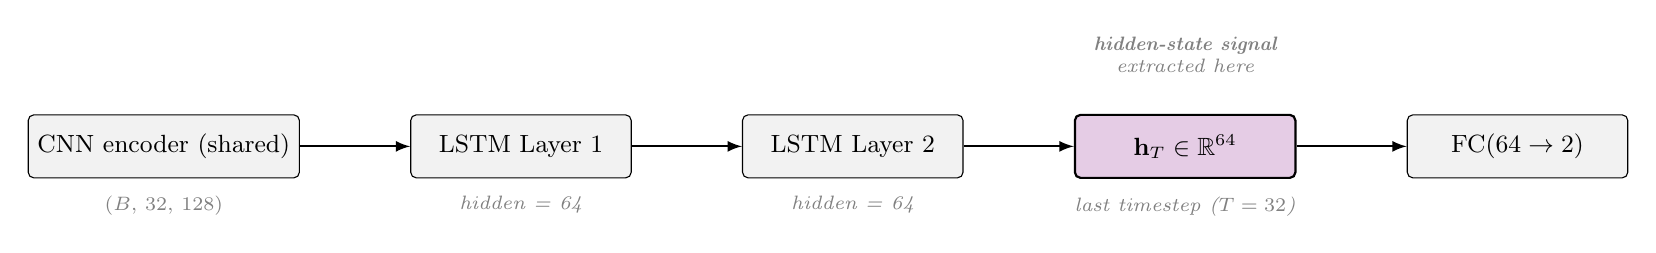
\begin{tikzpicture}[
    node distance=8mm and 14mm,
    box/.style={draw, rounded corners=2pt, minimum width=28mm, minimum height=8mm,
                font=\small, fill=gray!10},
    highlight/.style={draw, rounded corners=2pt, minimum width=28mm, minimum height=8mm,
                font=\small, fill=violet!20, thick},
    arr/.style={->, >=latex, thick},
    dim/.style={font=\scriptsize\itshape, text=gray},
  ]
  \node[box]       (cnn)   {CNN encoder (shared)};
  \node[dim, below=1mm of cnn] {$(B,\,32,\,128)$};
  \node[box, right=of cnn] (lstm1) {LSTM Layer 1};
  \node[dim, below=1mm of lstm1] {hidden = 64};
  \node[box, right=of lstm1] (lstm2) {LSTM Layer 2};
  \node[dim, below=1mm of lstm2] {hidden = 64};
  \node[highlight, right=of lstm2] (ht) {$\mathbf{h}_{T}\in\mathbb{R}^{64}$};
  \node[dim, below=1mm of ht] {last timestep ($T=32$)};
  \node[box, right=of ht] (fc) {FC$(64\to 2)$};
  \draw[arr] (cnn)   -- (lstm1);
  \draw[arr] (lstm1) -- (lstm2);
  \draw[arr] (lstm2) -- (ht);
  \draw[arr] (ht)    -- (fc);
  \node[dim, above=4mm of ht, align=center] {\textbf{hidden-state signal}\\extracted here};
\end{tikzpicture}%
}% end resizebox
\caption{Authentication model dataflow. The hidden-state signal $\delta_\text{hidden}(s)$
         is extracted from the last-timestep hidden state $\mathbf{h}_T \in \mathbb{R}^{64}$
         of the second LSTM layer, immediately before the FC classifier.}
\label{fig:lstm_arch}
\end{figure}

\FloatBarrier
\subsubsection{Centroid-Distance Formulation}
\label{ssec:mia_hidden_formula}

For a subject $s$, the pairs used to evaluate $\delta(s)$ in the output space can also be passed through the LSTM to obtain the last hidden state $\mathbf{h}_i \in \mathbb{R}^{64}$ for each pair $i$. The two pair types (genuine, $y=0$; impostor, $y=1$) partition these vectors into two clouds in the 64-dimensional representation space. The hidden centroid delta is:
\begin{equation}
  \delta_\text{hidden}(s)
  = \left\lVert
      \boldsymbol{\mu}_\text{imp}(s) - \boldsymbol{\mu}_\text{gen}(s)
    \right\rVert_2,
\end{equation}
where $\boldsymbol{\mu}_\text{imp}(s)$ and $\boldsymbol{\mu}_\text{gen}(s)$ are the centroids of the impostor- and genuine-pair hidden states respectively. Training pushes these centroids apart for enrolled subjects; taking the L2 norm between means (rather than per-pair distances) suppresses outlier pairs and measures whether the two clouds have separated as a whole.

\subsubsection{Results}
\label{ssec:mia_hidden_results}

Table~\ref{tab:hidden_delta} shows that the hidden-layer centroid delta tracks the output-space delta closely across all configurations. The additional dimensionality of $\mathbf{h}_T$ does not yield a stronger membership signal: because the final classifier is a single linear layer, centroid distance in the 64-dimensional hidden space and the scalar output distribution are related by the same learned projection. Any direction in $\mathbf{h}_T$ that separates member and non-member distributions must already be captured by that projection, so no new information is accessible at this layer beyond what the output score exposes.

\begin{table}[htbp]
\centering
\caption{Hidden-layer centroid delta results. Mean threshold uses no ground-truth labels (attacker-realistic). TPR values are coarse due to small non-member populations.}
\label{tab:hidden_delta}
\begin{tabular}{lrrr}
\toprule
Configuration & Hidden-$\delta$ AUC & Mean-thr TPR & Mean-thr FPR \\
\midrule
whuGAIT  & \whuGAITHiddenDeltaAUC  & \hiddenMeanTPR       & \hiddenMeanFPR       \\
UCI-HAR  & \uciharHiddenDeltaAUC   & \uciharHiddenMeanTPR & \uciharHiddenMeanFPR \\
WISDM    & \wisdmHiddenDeltaAUC    & \wisdmHiddenMeanTPR  & \wisdmHiddenMeanFPR  \\
Combined & \combinedHiddenDeltaAUC & \combinedHiddenMeanTPR & \combinedHiddenMeanFPR \\
\bottomrule
\end{tabular}
\end{table}

% ─────────────────────────────────────────────────────────────────────────────
\section{PGD Budget as Membership Signal}
\label{sec:mia_pgd_signal}

\subsubsection{Asymmetry Hypothesis}
\label{ssec:mia_pgd_hyp}

The minimum perturbation budget $\varepsilon_\text{min}$ established in Chapter~\ref{ch:evasion} for each impostor pair reflects how tightly the model's decision boundary encloses the genuine class for that subject. A model that has been trained on a subject's pairs places the genuine cluster in a highly structured, tightly bounded region of input space; an impostor needs a larger perturbation to cross that boundary. A held-out subject's genuine cluster, having never been fitted, is less tightly bounded, so impersonation requires less perturbation.

If this asymmetry holds across subjects, the per-subject mean $\bar{\varepsilon}_\text{min}(s)$ over all impostor pairs in which $s$ participates as the impostor functions as an aggregate membership signal: pairs drawn from the training split, where both subjects are enrolled, should require larger minimum budgets than pairs from the test split, where both subjects are held out.

Formally, for a subject $s$, let $\mathcal{A}_s$ be the set of impostor pairs in which $s$ acts as the impostor and that were successfully attacked within $\varepsilon_\text{max}$. The signal is:
\begin{equation}
  \bar{\varepsilon}_\text{min}(s)
  = \frac{1}{|\mathcal{A}_s|}
    \sum_{i \in \mathcal{A}_s} \varepsilon^{(i)}_\text{min}.
\end{equation}
Subjects for which $\mathcal{A}_s = \emptyset$ are excluded from the AUC computation. The signal is evaluated by comparing $\bar{\varepsilon}_\text{min}$ across enrolled subjects (from the training-split attack) and held-out subjects (from the test-split attack), using the same binary-search PGD protocol in both cases.

An important limitation of this design is that the two attack populations are not directly comparable. The training-split pairs have enrolled subjects on both sides of each pair (impostor and target), while the test-split pairs have held-out subjects on both sides. Consequently, it is not possible to isolate whether the $\varepsilon_\text{min}$ difference arises from the target subject being enrolled (the intended signal) or from the impostor subject also being enrolled. The signal is best interpreted as a group-level aggregate: training-split attacks are systematically harder than test-split attacks, rather than as a per-subject membership signal for the target subject specifically.

\subsubsection{Results}
\label{ssec:mia_pgd_results_v2}

\begin{table}[htbp]
\centering
\caption{PGD-budget membership signal AUC per dataset. Simple-$\delta$ AUC shown for comparison. Coverage notes are given in the text.}
\label{tab:pgd_mia_v2}
\begin{tabular}{lrr}
\toprule
Configuration & PGD-$\varepsilon$ AUC & Simple-$\delta$ AUC \\
\midrule
whuGAIT  & \whuGAITPgdMiaAUC  & \whuGAITSimplDAUC  \\
UCI-HAR  & \uciharPgdMiaAUC   & \uciharSimplDAUC   \\
WISDM    & \wisdmPgdMiaAUC    & \wisdmSimplDAUC    \\
Combined & \combinedPgdMiaAUC & \combinedSimplDAUC \\
\bottomrule
\end{tabular}
\end{table}

For UCI-HAR and WISDM, the training-split attack covered all available impostor combos, giving enrolled subjects a comparable number of attacked pairs to the held-out subjects. The resulting AUC values (\uciharPgdMiaAUC{} and \wisdmPgdMiaAUC{}) are therefore meaningful comparisons between member and non-member mean budgets under similar coverage.

For the combined configuration, the AUC of \combinedPgdMiaAUC{} is essentially random. The per-subject decision boundary is too loosely fitted in the cross-domain setting for the PGD budget to carry membership information, consistent with the lower output-space delta on that configuration.

The underlying limitation of this signal is structural: the coverage asymmetry between training-split and test-split attacks, combined with the confounded impostor/target membership status, makes the signal unreliable whenever the training set is large relative to the combo budget.

% ─────────────────────────────────────────────────────────────────────────────
\section{Signal Comparison}
\label{sec:mia_signal_comparison}

The output-space and hidden-layer deltas require only query and white-box access respectively; the PGD-budget signal additionally requires running the full adversarial attack pipeline from Chapter~\ref{ch:evasion} (Table~\ref{tab:signal_comparison}).

\begin{table}[htbp]
\centering
\caption{Comparison of the three shadow-free MIA signals. Output-$\delta$: black-box query access. Hidden-$\delta$: white-box activation access. PGD-$\varepsilon$: adversarial attack budget; coverage limitations apply for whuGAIT (see Section~\ref{ssec:mia_pgd_results_v2}).}
\label{tab:signal_comparison}
\begin{tabular}{lrrr}
\toprule
Configuration & Simple-$\delta$ AUC & Hidden-$\delta$ AUC & PGD-$\varepsilon$ AUC \\
\midrule
whuGAIT  & \whuGAITSimplDAUC  & \whuGAITHiddenDeltaAUC  & \whuGAITPgdMiaAUC  \\
UCI-HAR  & \uciharSimplDAUC   & \uciharHiddenDeltaAUC   & \uciharPgdMiaAUC   \\
WISDM    & \wisdmSimplDAUC    & \wisdmHiddenDeltaAUC    & \wisdmPgdMiaAUC    \\
Combined & \combinedSimplDAUC & \combinedHiddenDeltaAUC & \combinedPgdMiaAUC \\
\bottomrule
\end{tabular}
\end{table}

The delta signals dominate where coverage is sufficient: the PGD budget carries a confounded pair-level signal that cannot isolate individual subject membership. The hidden-layer delta adds no consistent gain, confirming that the linear classifier already exposes whatever the hidden state contains.

\begin{figure}[htbp]
  \centering
  \includegraphics[width=0.9\textwidth]{analysis/mia_new_signals_auc.png}
  \caption{AUC of the three shadow-free membership signals across datasets. The dashed line marks the random-classifier baseline.}
  \label{fig:new_signals_auc}
\end{figure}

\begin{figure}[htbp]
  \centering
  \includegraphics[width=\textwidth]{analysis/mia_new_signals_roc.png}
  \caption{ROC curves for the output-space delta (dashed) and hidden-layer centroid delta (solid purple) per dataset configuration.}
  \label{fig:new_signals_roc}
\end{figure}

% ─────────────────────────────────────────────────────────────────────────────
\section{LiRA Shadow Model Attack}
\label{sec:mia_lira}

\subsection{Shadow Model Training}
\label{ssec:mia_shadow_train}

The LiRA attack requires training $K$ shadow LSTM models, each on a different subset of the training pairs. The shadow models approximate the distribution of model behaviours when a target subject is excluded from training (OUT distribution), which is then used to assess how unusual the target model's delta is for that subject.

All shadow variants use the all-subjects split protocol. The full population of enrolled and held-out subjects is pooled together, and a random 50\% is drawn as the shadow-in set for each shadow $k$. Only pairs whose both windows come from subjects in the shadow-in set are used to train that shadow. Membership labels are not used during this assignment: the attacker has no prior knowledge of which subjects are members. For each target subject $s$, the OUT distribution is estimated from the shadows where $s$ fell outside the shadow-in set.

Each shadow is trained for 3 epochs with the Adam optimiser, using the same hyperparameters as the target model (learning rate $2.5 \times 10^{-3}$, weight decay $1.5 \times 10^{-3}$, dropout 0.3). Three epochs keeps shadow training tractable at $K = 32$; whether additional epochs would change the attack success is not evaluated.

\subsection{Likelihood Ratio Score}
\label{ssec:mia_lr_score}

For each target subject $s$, the $K$ shadow models that had $s$ in their OUT set provide samples of the delta distribution under the hypothesis that $s$ was not in training. Let $\delta^{\text{out}}_k(s)$ denote the delta computed from shadow $k$ for subject $s$, where $s \notin$ shadow $k$'s training set. A Gaussian is fitted to these samples:
\begin{equation}
  \mu^{\text{out}}(s),\; \sigma^{\text{out}}(s)
  \;=\; \text{MLE fit of }
  \bigl\{\delta^{\text{out}}_k(s)\bigr\}_{k:\, s \notin \text{train}_k}.
\end{equation}
The offline LiRA score (Equation~\eqref{eq:lira_offline} from Chapter~\ref{ch:background}) is then:
\begin{equation}
  \text{score}(s)
  = \Phi\!\bigl(\delta_{\text{target}}(s);\,
    \mu^{\text{out}}(s),\, \sigma^{\text{out}}(s)\bigr),
\end{equation}
where $\delta_{\text{target}}(s)$ is the delta computed from the target model. A score close to 1 means the target model produces a higher delta for $s$ than the OUT shadow distribution predicts, indicating membership.

\subsection{Threat Model Comparison}
\label{sec:mia_threat}

\subsubsection{Cold-Start Black-Box Attack}
\label{ssec:mia_cold}

The cold-start attacker knows only the model architecture. Each of the $K = 32$ shadow LSTMs is initialised independently from random Xavier weights and trained for 3 epochs on its shadow-in subset under the all-subjects protocol. There is no shared starting point between shadows, so the $K$ OUT delta samples for each subject span a wide range of independent model behaviours. This variety gives the Gaussian fit for the LiRA score a broader support and more reliable tails.

\subsubsection{Grey-Box Attack}
\label{ssec:mia_grey}

The grey-box attacker has access to the target model checkpoint. This is a stronger threat-model assumption than cold-start: the attacker not only knows the architecture but has the trained weights. Each shadow LSTM is initialised from those exact weights and fine-tuned for 3 epochs on its shadow-in subset under the all-subjects protocol. The hypothesis is that starting from the target model's prior gives the shadow a more informed starting distribution, sharpening the OUT Gaussian fit for each subject. In practice, the 3-epoch fine-tuning budget appears insufficient to escape this prior on whuGAIT, which likely explains the inverted signal observed there.

\subsubsection{Warm-Start Black-Box Attack}
\label{ssec:mia_warm}

Like cold-start, the warm-start attacker knows only the model architecture and has no access to the target checkpoint. The idea is to recover some of the grey-box efficiency saving without the stronger access assumption: the attacker first trains a single surrogate LSTM from random initialisation for 5 epochs on all available pairs (the full combined pool under the all-subjects protocol), then uses those surrogate weights as the shared starting point for all $K$ shadow models, each of which is fine-tuned for 3 epochs on its shadow-in subset. The question is whether a shared warm initialisation can reduce effective per-shadow training cost while still producing diverse enough OUT distributions for the LiRA score.

\subsubsection{Results and Discussion}
\label{ssec:mia_threat_results}

\begin{table}[htbp]
\centering
\caption{LiRA results (raw-$\delta$) by threat model. Results vary across datasets; each shadow is trained for 3 epochs (see Section~\ref{ssec:mia_threat_results}).}
\label{tab:threat_comparison}
\begin{tabular}{llrrrr}
\toprule
Config & Metric & Simple-$\delta$ & Grey & Warm & Cold \\
\midrule
\multirow{2}{*}{whuGAIT}
  & AUC          & \whuGAITSimplDAUC   & \whuGAITGreyLiraRawAUC  & \whuGAITWarmLiraRawAUC  & \whuGAITColdLiraRawAUC  \\
  & TPR at 10\% FPR  & \whuGAITSimplDTPRten & \whuGAITGreyLiraRawTPRten & \whuGAITWarmLiraRawTPRten & \whuGAITColdLiraRawTPRten \\
\multirow{2}{*}{UCI-HAR}
  & AUC          & \uciharSimplDAUC    & \uciharGreyLiraRawAUC   & \uciharWarmLiraRawAUC   & \uciharColdLiraRawAUC   \\
  & TPR at 10\% FPR  & \uciharSimplDTPRten  & \uciharGreyLiraRawTPRten  & \uciharWarmLiraRawTPRten  & \uciharColdLiraRawTPRten  \\
\multirow{2}{*}{WISDM}
  & AUC          & \wisdmSimplDAUC     & \wisdmGreyLiraRawAUC    & \wisdmWarmLiraRawAUC    & \wisdmColdLiraRawAUC    \\
  & TPR at 10\% FPR  & \wisdmSimplDTPRten   & \wisdmGreyLiraRawTPRten   & \wisdmWarmLiraRawTPRten   & \wisdmColdLiraRawTPRten   \\
\multirow{2}{*}{Combined}
  & AUC          & \combinedSimplDAUC  & \combinedGreyLiraRawAUC & \combinedWarmLiraRawAUC & \combinedColdLiraRawAUC \\
  & TPR at 10\% FPR  & \combinedSimplDTPRten & \combinedGreyLiraRawTPRten & \combinedWarmLiraRawTPRten & \combinedColdLiraRawTPRten \\
\bottomrule
\end{tabular}
\end{table}

Results vary across datasets and do not point to a single dominant strategy. On whuGAIT, warm-start is the strongest variant (\whuGAITWarmLiraRawAUC{}) followed by cold-start (\whuGAITColdLiraRawAUC{}), with grey-box the weakest (\whuGAITGreyLiraRawAUC{}). On UCI-HAR the pattern reverses between warm and cold: cold-start (\uciharColdLiraRawAUC{}) edges out warm-start (\uciharWarmLiraRawAUC{}). On WISDM, warm-start again leads (\wisdmWarmLiraRawAUC{} vs.\ cold \wisdmColdLiraRawAUC{}). On the combined configuration, both shadow variants outperform grey-box and simple-delta, with warm-start at \combinedWarmLiraRawAUC{}. Grey-box is consistently the weakest LiRA variant despite having the strongest access assumption: with only 3 epochs per shadow, fine-tuning from the target prior is insufficient to specialise the shadows, and the resulting OUT distribution is less diverse than what cold and warm-start produce from unconstrained random initialisation. TPR at 10\% FPR remains low across most configurations, limiting practical utility at a controlled false-positive rate. Given the 3-epoch shadow budget, these rankings should be read as indicative rather than definitive.

\begin{figure}[htbp]
  \centering
  \includegraphics[width=0.85\textwidth]{analysis/mia_nb05c_threat_models.png}
  \caption{LiRA AUC (raw-$\delta$) by threat model and dataset. The dashed line
           marks the random-classifier baseline (AUC $= 0.5$).}
  \label{fig:threat_models}
\end{figure}

\begin{figure}[htbp]
  \centering
  \includegraphics[width=\textwidth]{analysis/mia_roc_comparison.png}
  \caption{MIA ROC curves for simple-$\delta$ and LiRA variants (grey-box
           raw, cold-start raw, cold-start logit-first) across all four
           dataset configurations. AUC values are shown in the legend. The
           whuGAIT panel shows grey-box falling below the diagonal (inverted
           signal), while cold-start sits well above it.}
  \label{fig:mia_roc}
\end{figure}

% ─────────────────────────────────────────────────────────────────────────────
\section{Cold-Start Delta Variants}
\label{sec:mia_delta_variants}

Having established cold-start as the most effective and robust threat model, it remains to decide how to compute the delta score that feeds into the LiRA likelihood ratio. The original LiRA paper~\cite{carlini2022membership} applies a logit transform to the model's confidence before computing the membership statistic, which stabilises the tails of the score distribution for classification models. Here, the model outputs a pairwise probability rather than a classification confidence, so it is not obvious whether the same transformation is beneficial. Three formulations are tested.

\textbf{Raw} ($\delta_\text{raw}$): direct difference of mean scores,
$\bar{P}_\text{imp}(s) - \bar{P}_\text{gen}(s)$. Simple and interpretable, but the scale of the difference compresses near 0 and 1 where probabilities saturate.

\textbf{Logit-first} ($\delta_\text{lf}$): the logit transform is applied to
each individual pair score before computing the mean:
\begin{equation}
  \delta_\text{lf}(s)
  = \overline{\mathrm{logit}\!\left(P_\text{imp}(s)\right)}
  - \overline{\mathrm{logit}\!\left(P_\text{gen}(s)\right)}.
\end{equation}
This is the closest analogue to the original LiRA formulation: the logit is applied per sample before aggregation, stabilising scores at the extremes and giving greater weight to pairs where the model is highly confident.

\textbf{Mean-first} ($\delta_\text{mf}$): the logit is applied after computing
the mean:
\begin{equation}
  \delta_\text{mf}(s)
  = \mathrm{logit}\!\left(\bar{P}_\text{imp}(s)\right)
  - \mathrm{logit}\!\left(\bar{P}_\text{gen}(s)\right).
\end{equation}
This is more stable when the number of pairs per subject is small, because a single extreme pair score does not dominate the logit.

\begin{table}[htbp]
\centering
\caption{Cold-start LiRA results by delta variant. Simple-$\delta$ shown for reference.}
\label{tab:cold_variants}
\begin{tabular}{llrrrr}
\toprule
Config & Metric & Simple-$\delta$ & Cold-raw & Cold-lf & Cold-mf \\
\midrule
\multirow{2}{*}{whuGAIT}
  & AUC         & \whuGAITSimplDAUC   & \whuGAITColdLiraRawAUC  & \whuGAITColdLiraLfAUC  & \whuGAITColdLiraMfAUC  \\
  & TPR at 10\% FPR & \whuGAITSimplDTPRten & \whuGAITColdLiraRawTPRten & \whuGAITColdLiraLfTPRten & \whuGAITColdLiraMfTPRten \\
\multirow{2}{*}{UCI-HAR}
  & AUC         & \uciharSimplDAUC    & \uciharColdLiraRawAUC   & \uciharColdLiraLfAUC   & \uciharColdLiraMfAUC   \\
  & TPR at 10\% FPR & \uciharSimplDTPRten  & \uciharColdLiraRawTPRten  & \uciharColdLiraLfTPRten  & \uciharColdLiraMfTPRten  \\
\multirow{2}{*}{WISDM}
  & AUC         & \wisdmSimplDAUC     & \wisdmColdLiraRawAUC    & \wisdmColdLiraLfAUC    & \wisdmColdLiraMfAUC    \\
  & TPR at 10\% FPR & \wisdmSimplDTPRten   & \wisdmColdLiraRawTPRten   & \wisdmColdLiraLfTPRten   & \wisdmColdLiraMfTPRten   \\
\multirow{2}{*}{Combined}
  & AUC         & \combinedSimplDAUC  & \combinedColdLiraRawAUC & \combinedColdLiraLfAUC & \combinedColdLiraMfAUC \\
  & TPR at 10\% FPR & \combinedSimplDTPRten & \combinedColdLiraRawTPRten & \combinedColdLiraLfTPRten & \combinedColdLiraMfTPRten \\
\bottomrule
\end{tabular}
\end{table}

Raw and mean-first perform similarly across datasets. Logit-first is generally weaker, possibly because gait pair scores cluster near 0 and 1 more than classification confidences do, making the per-pair logit numerically unstable for a larger fraction of pairs. Figure~\ref{fig:cold_variants} shows the three formulations side by side.

\begin{figure}[htbp]
  \centering
  \includegraphics[width=0.85\textwidth]{analysis/mia_nb05c_cold_variants.png}
  \caption{Cold-start LiRA AUC by delta variant (raw, logit-first, mean-first)
           across all four configurations. Raw and mean-first track closely;
           logit-first underperforms on the combined run.}
  \label{fig:cold_variants}
\end{figure}

% ─────────────────────────────────────────────────────────────────────────────
\section{Signal Disentanglement}
\label{sec:mia_signal}

\subsection{Motivation and Design}
\label{ssec:mia_signal_design}

The experiments in the preceding sections train both the CNN encoder and the authentication LSTM on the same subject pool, so any measured membership signal could originate from either component. The CNN may have memorised the gait representations of its training subjects during classification pre-training; the LSTM may have fitted the pair-score distribution of its own training subjects during authentication training. These two contributions are inseparable in the standard pipeline.

To disentangle them, the pipeline is re-run on the \texttt{whuGAIT\_signal} variant, which uses 116 of the 118 available whuGAIT Dataset~1 subjects and partitions them into four contiguous non-overlapping groups of 29 before any training:

\begin{table}[htbp]
\centering
\caption{Subject group assignment for the signal disentanglement experiment (29 subjects per group).}
\label{tab:signal_design}
\begin{tabular}{lccl}
\toprule
Group & Subjects & CNN trained & LSTM trained \\
\midrule
A &   1--29  & yes & no  \\
B &  30--58  & no  & yes \\
C &  59--87  & no  & no  \\
D &  88--116 & yes & yes \\
\bottomrule
\end{tabular}
\end{table}

Group~A isolates the CNN encoder's contribution: the encoder has shaped their gait representations, but the authentication LSTM has never seen them. Group~B isolates the LSTM's contribution: the LSTM has fitted their pair scores directly, but the CNN treats them as unseen subjects with generic embeddings. Group~C is the held-out baseline that neither component trained on. Group~D trains both components on the same subjects; if the combined signal from~D exceeds the maximum of the individual signals from~A and~B, the two components act super-additively.

\subsection{Authentication Performance per Group}
\label{ssec:mia_signal_auth}

Before examining the MIA signal, the authentication model's discrimination quality is characterised per group. All groups are evaluated using the same trained model; the differences reflect how much each group's gait representations were shaped by training.

\begin{table}[htbp]
\centering
\caption{Authentication AUC per group in the signal disentanglement experiment.}
\label{tab:signal_auth}
\begin{tabular}{llr}
\toprule
Group & Role & Auth AUC \\
\midrule
C (59--87)  & held-out baseline & \signalAuthModelAUCC \\
A (1--29)   & CNN-only          & \signalAuthModelAUCA \\
B (30--58)  & LSTM-only         & \signalAuthModelAUCB \\
D (88--116) & both              & \signalAuthModelAUCD \\
\bottomrule
\end{tabular}
\end{table}

Group~A sits above the held-out baseline despite the LSTM never having trained on their pairs, confirming that the CNN encoder's prior representation of those subjects carries a measurable advantage for the authentication head. Figure~\ref{fig:signal_auth} shows the per-group AUC and accuracy.

\begin{figure}[htbp]
  \centering
  \includegraphics[width=0.85\textwidth]{analysis/signal_auth_performance.png}
  \caption{Authentication model AUC and accuracy per subject group.
           Group~A exceeds the held-out baseline (Group~C) despite
           the LSTM having no direct training on those subjects, reflecting the
           CNN encoder's prior gait representations.}
  \label{fig:signal_auth}
\end{figure}

\subsection{MIA Signal per Group}
\label{ssec:mia_signal_results}

\begin{table}[htbp]
\centering
\caption{Signal disentanglement MIA AUC. Each group is scored against Group~C (held-out baseline).
         D/C tests whether the joint signal is super-additive.}
\label{tab:signal_mia}
\small
\begin{tabular}{lrrr}
\toprule
Attack & B\,vs\,C (LSTM) & A\,vs\,C (CNN) & D\,vs\,C (both) \\
\midrule
Simple-$\delta$  & \signalMiaAUCBvsC    & \signalMiaAUCAvsC    & \signalMiaAUCDvsC    \\
\bottomrule
\end{tabular}
\end{table}

Both Group~A and Group~B produce AUC above chance, confirming that each component independently contributes a membership signal. The magnitude of the two signals (\signalMiaAUCBvsC{} for the LSTM vs.\ \signalMiaAUCAvsC{} for the CNN) indicates their relative contributions.

\paragraph{Interaction test.}
If the CNN and LSTM memorisation signals were strictly additive, Group~D's signal should not exceed the larger of the A/C and B/C signals. The interaction difference $\text{AUC}(D/C) - \max(\text{AUC}(A/C),\,\text{AUC}(B/C)) = \signalMiaInteractionDiff{}$ quantifies whether the joint group shows super-additive leakage. A positive value would indicate the two components reinforce each other; a negative or near-zero value indicates that the signals do not compound.

\paragraph{Operating-point analysis.}
Setting the decision threshold to maintain $\text{FPR} = 0.10$ on Group~C yields the attack rates per group shown in Figure~\ref{fig:signal_confusion}. The threshold (\signalConfusionThresholdFPRTen{}) is derived from the 90th percentile of Group~C delta scores. Groups that exceed this threshold more than 10\% of the time carry more information about their subjects than can be explained by within-subject gait variability alone.

\begin{figure}[htbp]
  \centering
  \includegraphics[width=0.85\textwidth]{analysis/signal_confusion_per_group.png}
  \caption{Attack outcome per group at a fixed FPR = 0.10 operating point
           (threshold set on Group~C). Each group has 29 subjects. Groups~A
           and~B show elevated predicted-member rates relative to Group~C,
           reflecting the CNN and LSTM memorisation signals respectively.}
  \label{fig:signal_confusion}
\end{figure}

Figure~\ref{fig:signal_auc_bar} shows the mean percentile rank of each group under two attack variants: simple-$\delta$ and LiRA-raw (grey-box). Shadow-based black-box attacks (cold-start, warm-start) are not included in the disentanglement analysis: a shadow set must be calibrated against a single consistent membership definition, but the 2$\times$2 design defines membership differently for each comparison (CNN training, authenticator training, or both). The simple-$\delta$ and grey-box LiRA, both of which use the target model directly, are the appropriate tools here.

\begin{figure}[htbp]
  \centering
  \includegraphics[width=0.85\textwidth]{analysis/signal_mia_auc_per_group.png}
  \caption{Mean percentile rank of MIA attack score by subject group and attack
           variant. The random baseline is 0.25 (four equal groups). Groups~A
           and~B sitting above this baseline confirm independent memorisation
           contributions from the CNN and LSTM components respectively.}
  \label{fig:signal_auc_bar}
\end{figure}

\subsection{Factorial Interaction}
\label{ssec:mia_signal_interaction}

Figure~\ref{fig:signal_interaction} presents the 2$\times$2 interaction plot and the per-subject delta score distribution. The interaction line plot shows two lines: one tracing the effect of adding CNN training when the LSTM is absent (C$\to$A), and one tracing the same CNN effect when the LSTM is present (B$\to$D). Parallel lines indicate an additive relationship between the two training factors; converging or crossing lines indicate an interaction.

\begin{figure}[htbp]
  \centering
  \includegraphics[width=\textwidth]{analysis/signal_interaction_strip.png}
  \caption{Left: interaction plot for the signal disentanglement experiment. The two lines show the
           effect of CNN training in the absence (C$\to$A) and presence (B$\to$D)
           of LSTM training. Parallel lines indicate an additive effect;
           deviation from parallelism measures the interaction term
           $(\signalMiaInteractionDiff{})$.
           Right: per-subject delta score distribution by group. Each point is
           one subject; the bar marks the group mean $\pm$ 1 standard deviation.}
  \label{fig:signal_interaction}
\end{figure}



% Chapter 7 — Continual Learning and Membership Inference
% Analyses whether the CDML continual-learning scheme reduces MIA vulnerability
% when an LSTM authenticator is built on top of the CL-trained CNN backbone.

% Auto-generated by nb08b_cl_authenticator: DO NOT EDIT MANUALLY
% Last run: 2026-09-28 11:22:40

\providecommand{\clAuthStdTaskZero}{}
\renewcommand{\clAuthStdTaskZero}{94.85\%}
\providecommand{\clAuthCdmlTaskZero}{}
\renewcommand{\clAuthCdmlTaskZero}{95.45\%}
\providecommand{\clAuthStdTaskOne}{}
\renewcommand{\clAuthStdTaskOne}{90.45\%}
\providecommand{\clAuthCdmlTaskOne}{}
\renewcommand{\clAuthCdmlTaskOne}{89.80\%}
\providecommand{\clAuthStdTaskTwo}{}
\renewcommand{\clAuthStdTaskTwo}{92.85\%}
\providecommand{\clAuthCdmlTaskTwo}{}
\renewcommand{\clAuthCdmlTaskTwo}{92.35\%}
\providecommand{\clAuthStdTaskThree}{}
\renewcommand{\clAuthStdTaskThree}{92.00\%}
\providecommand{\clAuthCdmlTaskThree}{}
\renewcommand{\clAuthCdmlTaskThree}{93.50\%}
\providecommand{\clAuthStdMean}{}
\renewcommand{\clAuthStdMean}{92.54\%}
\providecommand{\clAuthCdmlMean}{}
\renewcommand{\clAuthCdmlMean}{92.77\%}


\chapter{Continual Learning and Membership Inference}
\label{ch:cl_mia}

The pairwise LSTM authenticator operates in open-set mode: it scores any two windows without requiring prior enrolment, so new subjects can be authenticated without retraining. Continual learning is not a functional requirement here; it is a privacy variable. The hypothesis is that training the CNN encoder incrementally across subject groups reduces the per-subject memorisation that drives the MIA signal. This chapter tests that hypothesis by comparing a standard sequential backbone with a CDML backbone (Section~\ref{ssec:bg_cdml}) and measuring the effect on MIA AUC. The CNN encoder of Milani~\cite{milani2024gait} is trained across four sequential tasks of 24 subjects each, and an LSTM authenticator is trained on the frozen backbone.

The AUC gap between the two backbones is \clMiaCLMIAAUCGap{} (standard CL: \clMiaCLMIAStdAUC{}; CDML: \clMiaCLMIACdmlAUC{}). The CDML modulation is applied after the feature-map tap used by the authenticator, so the LSTM never receives a modulated embedding and the MIA surface is unchanged. The per-subject boundary calibration that authentication requires is the same signal the MIA exploits: any scheme that substantially reduces that signal also degrades authentication, bounding what any CL mechanism can achieve here.

% ─────────────────────────────────────────────────────────────────────────────
\section{CDML and Attacker Model}
\label{sec:cl_cdml}

The LSTM authenticator built on top of the CL backbone calls \texttt{get\_feature\_maps()}, which taps the convolutional feature maps after the fourth convolutional block and before the flatten layer. At this point the convolutional feature tensor has shape $(B,\,128,\,1,\,16)$, which the LSTM receives as a sequence of $16$ frames of 128-dimensional feature vectors per window. The modulation $\mathbf{s}_k$ is applied after the flatten layer, downstream of this tap. The LSTM therefore receives unmodulated feature maps regardless of which code, if any, is active in the identification head. The attacker's position is identical: they query the authenticator output without needing to know or use any code. Figure~\ref{fig:cdml_arch} illustrates the full data path.

\begin{figure}[htbp]
  \centering
  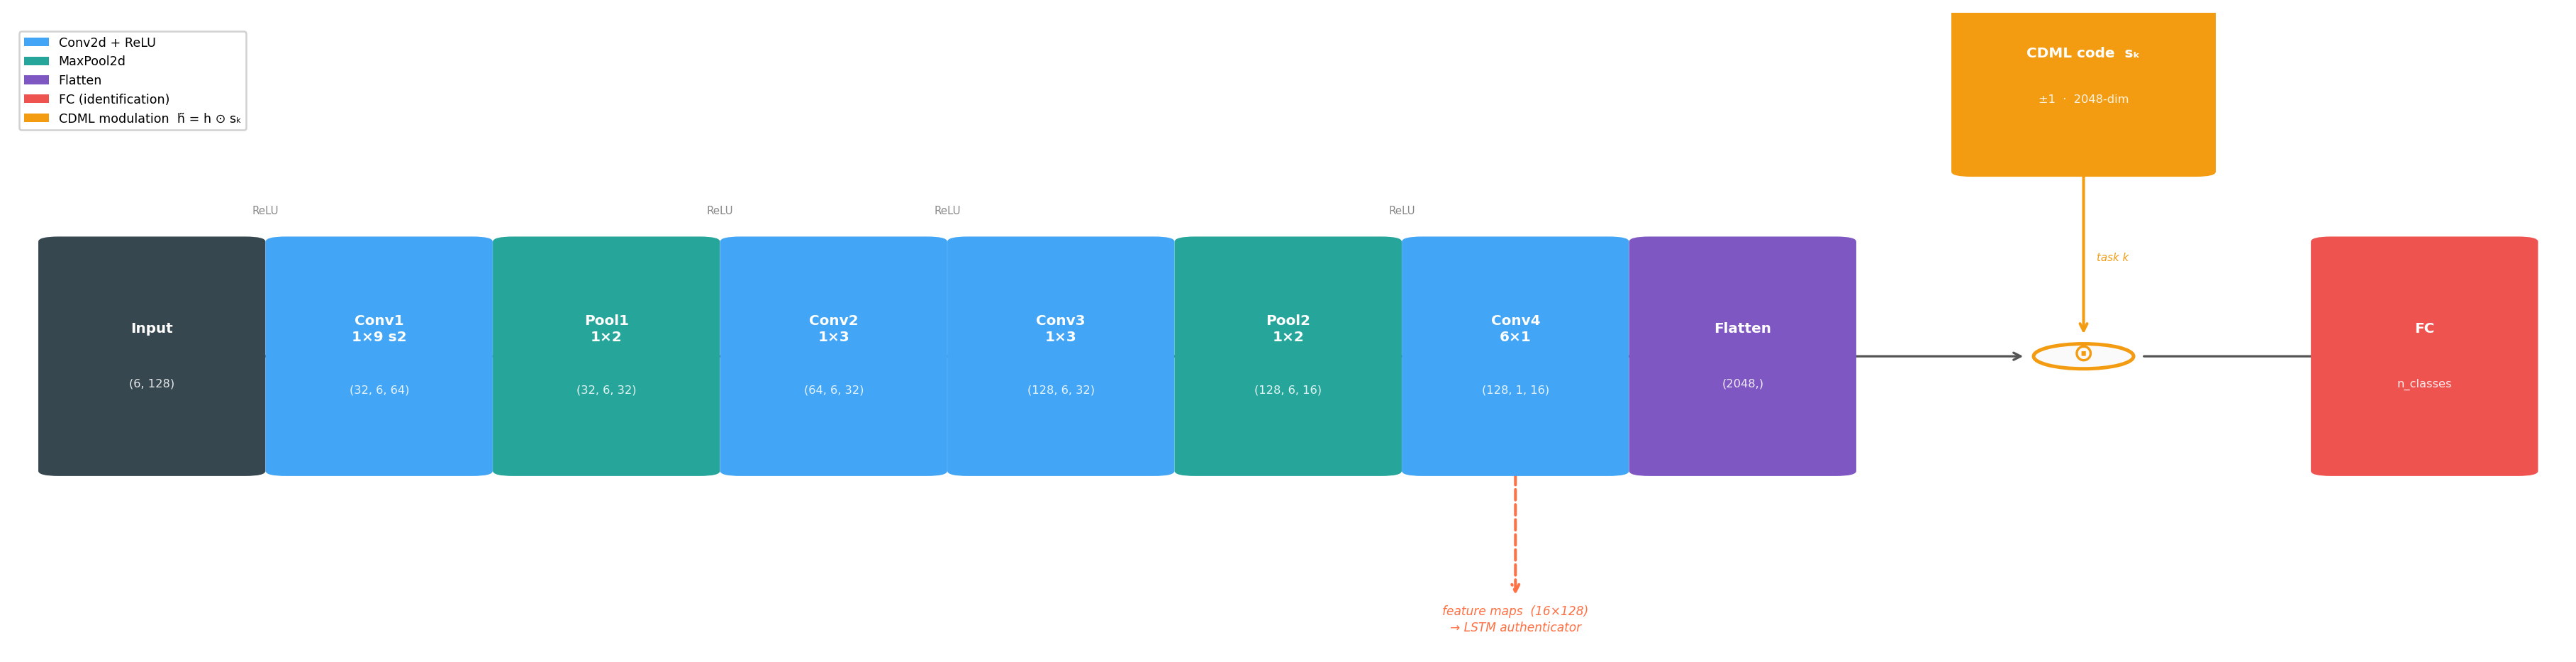
\includegraphics[width=\textwidth]{cdml_architecture.png}
  \caption{CDML encoder architecture. The task-specific binary code $\mathbf{s}_k \in \{-1,+1\}^{2048}$ is injected after the flatten layer, before the FC identification head ($\tilde{\mathbf{h}} = \mathbf{h} \odot \mathbf{s}_k$). The LSTM authenticator taps the convolutional feature maps at the Conv4 output, upstream of the modulation point, and therefore never receives the code.}
  \label{fig:cdml_arch}
\end{figure}

% ─────────────────────────────────────────────────────────────────────────────
\section{Experimental Setup}
\label{sec:cl_setup}

\subsection{Task Design}
\label{ssec:cl_tasks}

The 118 whuGAIT subjects are partitioned as follows. The 98 subjects that serve as members in the standard experiment (Chapter~\ref{ch:system}) are divided into four sequential tasks of 24 subjects each, yielding 96 member subjects across the four tasks. The 2 remaining subjects from the 98-member pool are treated as additional non-members, joining the 20 held-out subjects to form a non-member pool of 22 subjects. Table~\ref{tab:cl_split} summarises the partition.

\begin{table}[htbp]
\centering
\caption{Subject partition for the CL experiment.}
\label{tab:cl_split}
\begin{tabular}{lrl}
\toprule
Role & Subjects & Source \\
\midrule
Task 0 members & 24 & whuGAIT training split \\
Task 1 members & 24 & whuGAIT training split \\
Task 2 members & 24 & whuGAIT training split \\
Task 3 members & 24 & whuGAIT training split \\
Held-out non-members & 20 & whuGAIT Dataset~2 \\
Leftover non-members &  2 & whuGAIT training split (unassigned) \\
\midrule
Total members       & 96 & \\
Total non-members   & 22 & \\
\bottomrule
\end{tabular}
\end{table}

To eliminate task-size confounds in the MIA comparison, the training windows for each task are subsampled to the minimum window count across all four tasks before training begins. The four tasks have 6{,}257, 7{,}116, 6{,}386, and 6{,}661 training windows respectively; all tasks are subsampled to 6{,}257 windows. Subsampling is performed once per task using a fixed random seed and held constant across the std and CDML runs.

\subsection{Training Protocol}
\label{ssec:cl_training}

Two methods are compared:
\begin{itemize}
  \item \textbf{Std} (naive fine-tuning): the CNN is trained on each task in sequence with no mechanism to prevent forgetting. The classification head outputs over all 96 classes, but gradient updates from task $k$ overwrite representations learned during earlier tasks.
  \item \textbf{CDML}: before each task, a binary code $\mathbf{s}_k$ is generated from seed $1000 + k$ and registered. The modulated embedding $\tilde{\mathbf{h}} = \mathbf{h} \odot \mathbf{s}_k$ is passed to the FC head during task $k$ training. The codes from all previous tasks remain registered for evaluation.
\end{itemize}

Both methods use the Adam optimiser with initial learning rate $10^{-3}$ and batch size 512, matching the single-task CNN (Chapter~\ref{ch:system}). Because each task spans only 24 subjects and training runs for 100 epochs per task, an exponential learning rate schedule ($\gamma = 0.9$ per epoch) is added to provide stronger regularisation as the model converges deeper into each task's small data distribution.

After CL training, the encoder is frozen and an LSTM authenticator is trained on top of it using the same procedure and hyperparameters as Chapter~\ref{ch:system}. The checkpoint with the best test-set accuracy is retained. As discussed in Section~\ref{ssec:sys_auth_train}, selecting on the non-member test set is a conservative bias: the saved model generalises better to held-out subjects and is therefore less overfit to its training subjects, producing a weaker MIA signal. The reported AUCs are a lower bound.

\subsection{Attacker Model}
\label{ssec:cl_attacker}

The attacker knows the LSTM architecture and has black-box query access to the authenticator. They do not know any CDML code and do not know which subjects belong to which task. The attack is the simple delta-MIA from Chapter~\ref{ch:mia}: for each subject $s$, the delta score is computed from gait windows not necessarily seen during training:
\begin{equation}
  \delta(s) = \bar{P}_{\text{imp}}(s) - \bar{P}_{\text{gen}}(s).
\end{equation}
The 96 member subjects form the positive class and the 22 non-member subjects form the negative class. AUC is reported over the binary classification of all 118 subjects by their delta scores.

% ─────────────────────────────────────────────────────────────────────────────
\section{Continual Learning Results}
\label{sec:cl_results}

\subsection{Forgetting Curves}
\label{ssec:cl_forgetting}

The std model loses all Task-0 accuracy after the first sequential update (0\% from Task 1 onward). CDML retains it throughout, dipping to 81.5\% after Task 2 before recovering to 92.8\% at the end of Task 3 (Table~\ref{tab:cl_forgetting}).

\begin{table}[htbp]
\centering
\caption{Task-0 evaluation accuracy after each sequential training step. Std suffers complete catastrophic forgetting from Task 1 onward. CDML retains Task-0 accuracy throughout.}
\label{tab:cl_forgetting}
\begin{tabular}{lrr}
\toprule
Evaluation point & Std Task-0 acc & CDML Task-0 acc \\
\midrule
After Task 0 & 96.5\% & 96.6\% \\
After Task 1 &  0.0\% & 91.8\% \\
After Task 2 &  0.0\% & 81.5\% \\
After Task 3 &  0.0\% & 92.8\% \\
\bottomrule
\end{tabular}
\end{table}

The transient dip at Task 2 reflects imperfect code-based separation: interference accumulates over sequential updates before partly reversing when Task 3 representations are established.

\begin{figure}[htbp]
  \centering
  \includegraphics[width=\textwidth]{whuGAIT/08a_cl_forgetting.png}
  \caption{Left: Task-0 accuracy after each sequential training step, showing catastrophic forgetting in the std model and near-complete retention in CDML. Right: mean accuracy over all tasks seen so far. The std model's mean accuracy is carried entirely by the most recent task; CDML's mean accuracy reflects genuine multi-task retention.}
  \label{fig:cl_forgetting}
\end{figure}

% ─────────────────────────────────────────────────────────────────────────────
\section{Authentication on the CL Backbone}
\label{sec:cl_auth}

The LSTM authenticator is trained identically for both backbones with the CNN frozen. Test accuracy is 76.7\% (std) vs.\ 77.7\% (CDML): a small gap despite the std model retaining only Task-3 features, because those features alone support a useful authentication function. CDML's marginal advantage comes from the richer multi-task representation available to the authenticator.

\begin{table}[htbp]
\centering
\caption{Per-task LSTM authentication accuracy. Each task's accuracy is evaluated on pairs drawn from that task's 24 subjects. Non-member accuracy (test) uses the 22 held-out subjects.}
\label{tab:cl_auth}
\begin{tabular}{lrr}
\toprule
Evaluation set & Std LSTM & CDML LSTM \\
\midrule
Task 0 (subjects 1--24)   & \clAuthStdTaskZero  & \clAuthCdmlTaskZero  \\
Task 1 (subjects 25--48)  & \clAuthStdTaskOne   & \clAuthCdmlTaskOne   \\
Task 2 (subjects 49--72)  & \clAuthStdTaskTwo   & \clAuthCdmlTaskTwo   \\
Task 3 (subjects 73--96)  & \clAuthStdTaskThree & \clAuthCdmlTaskThree \\
\midrule
Mean (members)            & \clAuthStdMean      & \clAuthCdmlMean      \\
Test (non-members, all)   & 76.7\% & 77.7\% \\
\bottomrule
\end{tabular}
\end{table}

\begin{figure}[htbp]
  \centering
  \includegraphics[width=0.85\textwidth]{whuGAIT/08b_auth_per_task.png}
  \caption{Per-task LSTM authentication accuracy for the std and CDML backbones. The dashed lines mark the per-method mean. The std backbone's accuracy on Tasks 0--2 is lower because the encoder's representations for those subjects have been overwritten by subsequent training.}
  \label{fig:cl_auth_per_task}
\end{figure}

% ─────────────────────────────────────────────────────────────────────────────
\section{Delta-MIA Results}
\label{sec:cl_mia_results}

\subsection{Main Results}
\label{ssec:cl_mia_main}

\begin{table}[htbp]
\centering
\caption{Delta-MIA results for std and CDML backbones. Member $\delta$ is the mean delta score over the 96 member subjects; NM $\delta$ is the mean over the 22 non-member subjects. Separation is their difference. AUC is the area under the ROC curve over all 118 subjects.}
\label{tab:cl_mia_main}
\begin{tabular}{lrrrr}
\toprule
Backbone & MIA AUC & Member $\delta$ & NM $\delta$ & Separation \\
\midrule
Std  & \clMiaCLMIAStdAUC  & \clMiaCLMIAStdMemDelta  & \clMiaCLMIAStdNMDelta  & \clMiaCLMIAStdSep  \\
CDML & \clMiaCLMIACdmlAUC & \clMiaCLMIACdmlMemDelta & \clMiaCLMIACdmlNMDelta & \clMiaCLMIACdmlSep \\
\bottomrule
\end{tabular}
\end{table}

CDML produces a higher MIA AUC than std (\clMiaCLMIACdmlAUC{} vs.\ \clMiaCLMIAStdAUC{}). The member mean delta rises from \clMiaCLMIAStdMemDelta{} to \clMiaCLMIACdmlMemDelta{}, while the non-member mean delta falls slightly from \clMiaCLMIAStdNMDelta{} to \clMiaCLMIACdmlNMDelta{}. Both effects widen the member--non-member separation from \clMiaCLMIAStdSep{} to \clMiaCLMIACdmlSep{}.

The std model's lower AUC is not evidence of better privacy. The std backbone has forgotten Tasks 0--2 entirely, so the authenticator's representations for those subjects' gait patterns are degraded. Members assigned to Tasks 0--2 produce lower delta scores not because their membership is harder to infer in principle, but because the underlying CNN representations are less coherent. This confounds the comparison: the std baseline benefits from forgetting-induced noise that suppresses the membership signal, but this suppression is inseparable from reduced authentication utility.

\begin{figure}[htbp]
  \centering
  \includegraphics[width=\textwidth]{whuGAIT/08c_delta_distributions.png}
  \caption{Delta score distributions for member subjects (coloured) and non-member subjects (grey) for the std (left) and CDML (right) backbones. The CDML distribution shows a wider separation between the two populations, consistent with the higher MIA AUC.}
  \label{fig:cl_delta_distributions}
\end{figure}

\begin{figure}[htbp]
  \centering
  \includegraphics[width=0.7\textwidth]{whuGAIT/08c_mia_roc.png}
  \caption{Delta-MIA ROC curves for std and CDML backbones. CDML sits substantially above the std curve at all operating points. AUC values are shown in the legend.}
  \label{fig:cl_mia_roc}
\end{figure}

\subsection{Comparison with the Standard Single-Task Experiment}
\label{ssec:cl_mia_comparison}

In the standard whuGAIT experiment (Chapter~\ref{ch:mia}), the simple-delta MIA AUC against the single-task authenticator is \whuGAITSimplDAUC{}. The CDML backbone in the CL setting achieves \clMiaCLMIACdmlAUC{}, which is higher. Part of this difference is attributable to the larger member pool (96 vs.\ 98 subjects) and the different non-member pool (22 vs.\ 20 subjects); however, the direction of the difference is consistent with the hypothesis that CDML representations are more subject-specific at the feature-map level. The std baseline (\clMiaCLMIAStdAUC{}) is lower than the single-task result, reflecting the representation degradation from forgetting.

% ─────────────────────────────────────────────────────────────────────────────
\section{Per-Task Analysis}
\label{sec:cl_pertask}

\subsection{Forgetting and MIA Vulnerability over Tasks}
\label{ssec:cl_timeline}

Figure~\ref{fig:cl_timeline} overlays Task-0 retention accuracy and per-task MIA AUC (each task's 24 members vs.\ the full non-member pool) against the sequential task index. A per-task AUC above 0.5 means those members are more detectable than non-members when the attack is restricted to that task.

\begin{figure}[htbp]
  \centering
  \includegraphics[width=0.85\textwidth]{whuGAIT/08c_forgetting_mia_timeline.png}
  \caption{Task-0 retention accuracy (dashed, left axis) and per-task MIA AUC (solid, right axis) plotted against the sequential task index, for std (red) and CDML (blue). For the std model, both curves collapse after Task 0. For the CDML model, the per-task MIA AUC remains elevated throughout, matching the pattern of the retention curve.}
  \label{fig:cl_timeline}
\end{figure}

For the CDML backbone, the per-task MIA AUC follows the same qualitative pattern as the Task-0 retention: tasks whose representations are better preserved produce a stronger membership signal. Task 2 shows the smallest retention (81.5\%) and, correspondingly, a weaker MIA signal for those subjects; Tasks 0 and 3 show the highest retention and the strongest per-task attack. For the std backbone, the per-task MIA AUC collapses after Task 0 in the same way as the retention accuracy, confirming that the signal suppression is a byproduct of forgetting rather than a privacy property.

\subsection{Authentication Accuracy vs.\ MIA AUC}
\label{ssec:cl_scatter}

Figure~\ref{fig:cl_scatter} plots the per-task authentication accuracy against the per-task MIA AUC, with one point per task per backbone. The two quantities are positively correlated: tasks where the authenticator performs better are also the tasks where the membership signal is stronger. This positive relationship holds for both backbones and is consistent with the conclusion that both authentication accuracy and MIA vulnerability are driven by the same underlying quantity, namely how well the backbone has retained subject-specific representations.

\begin{figure}[htbp]
  \centering
  \includegraphics[width=0.7\textwidth]{whuGAIT/08c_scatter_auth_mia.png}
  \caption{Authentication accuracy vs.\ per-task MIA AUC for std (red circles) and CDML (blue squares), one point per task. Points are labelled T0--T3. The positive correlation between authentication utility and MIA vulnerability holds within each backbone.}
  \label{fig:cl_scatter}
\end{figure}

% ─────────────────────────────────────────────────────────────────────────────
\section{Discussion}
\label{sec:cl_discussion}

The main finding of this chapter is that CDML's privacy guarantee does not extend to the authentication layer when the LSTM taps the CNN at the feature-map level. The code $\mathbf{s}_k$ is applied after the tap point, so modifying its value has no effect on what the LSTM receives and no effect on the attacker's observations.

The indirect effect of CDML on MIA runs in the opposite direction from what a naive privacy argument would predict. CDML prevents catastrophic forgetting, which means the CNN representations for all four tasks remain informative and subject-specific. This is exactly the property that makes the authenticator more accurate and simultaneously makes the membership signal stronger: the LSTM can discriminate member genuine pairs from member impostor pairs more reliably, producing larger deltas for members relative to non-members.

The finding generalises the signal disentanglement result from Section~\ref{sec:mia_signal}. That experiment showed that the CNN encoder contributes an independent membership signal through the authentication head by shaping subject-specific representations. The CL experiment shows that an encoder trained to retain more subject-specific representations across a longer sequence of tasks produces a proportionally stronger signal.

One practical implication concerns continual learning deployments where privacy is a stated goal. If CDML is deployed to protect the identification head, the authentication component built on the same backbone inherits an increased privacy risk compared with a baseline that allows forgetting. Protecting the authentication layer would require either applying the code modulation at or before the feature-map tap point used by the authenticator, or training a separate authenticator whose feature extraction is not shared with the CL backbone.

% ─────────────────────────────────────────────────────────────────────────────


\chapter{Conclusions}
\label{ch:conclusions}

\section{Summary of Contributions}
\label{sec:con_summary}

\section{Limitations}
\label{sec:con_limitations}

\section{Future Work}
\label{sec:con_future}


% ── bibliography ──────────────────────────────────────────────────────────────
\bibliographystyle{plain}
\bibliography{references}

\end{document}
